\documentclass[11pt,a4paper]{report}
\usepackage[top=25mm,bottom=25mm,right=25mm,left=30mm,head=12.5mm,foot=12.5mm]{geometry}
\let\openright=\clearpage

%%% Tento soubor obsahuje definice různých užitečných maker a prostředí %%%
%%% Další makra připisujte sem, ať nepřekáží v ostatních souborech.     %%%

\usepackage{etoolbox}
\def\Jazyk{cze}
\def\ProhlaseniAIText{Prohlášení k~využití AI}
\let\ifstringequal\ifdefstring

% xurl musí být před hyperref (načítá ho pdfx), aby šly lámat dlouhé cesty a URL
\usepackage{xurl}
\usepackage{needspace}
\usepackage[a-2u]{pdfx}     % výsledné PDF bude ve standardu PDF/A-2u


%% Přepneme na českou sazbu, fonty Latin Modern a kódování češtiny
\usepackage[czech]{babel}
\usepackage{lmodern}
\usepackage{microtype}
\usepackage[T1]{fontenc}
\usepackage{textcomp}
\usepackage[utf8]{inputenc}
\usepackage{csquotes}

\appto{\bibsetup}{\sloppy}
\makeatletter
\def\UrlBigBreaks{\do\:}
\def\UrlBreaks{\do\/\do\.\do\-\do\?\do\,\do\_\do\%\do\=\do\#\do\~\do\&}
\makeatother

%%% Nastavení pro použití samostatné bibliografické databáze.
\usepackage[
   backend=biber
  ,style=apa
  ,apamaxprtauth=99
  %,sortlocale=cs_CZ
  ,sorting=nyt
  ,maxbibnames=20
  ,bibencoding=UTF8
]{biblatex}
\addbibresource{literatura.bib}
% Oficiální biblatex-apa neobsahuje czech-apa.lbx; v adresáři tex/ je odvozený soubor.
% Bez mapování na *-apa.lbx se v citacích místo roku vypisují názvy polí (např. labelday).
\DeclareLanguageMapping{czech}{czech-apa}
% V českém textu spojka mezi autory: „a“, ne anglické „and“ (i u stylu APA v těle práce).
\DefineBibliographyStrings{czech}{and = {a}}
\DeclareDelimFormat{finalnamedelim}{%
  \ifnumgreater{\value{listcount}}{\value{liststop}-1}
    {\addspace\bibstring{and}\space}
    {\addcomma\space}%
}

%%% Další užitečné balíčky (jsou součástí běžných distribucí LaTeXu)
\usepackage{amsmath}        % rozšíření pro sazbu matematiky
\usepackage{amsfonts}       % matematické fonty
\usepackage{amssymb}          % \checkmark a další symboly
\usepackage{amsthm}         % sazba vět, definic apod.
\usepackage{bm}             % tučné symboly (příkaz \bm)
\usepackage{graphicx}       % vkládání obrázků
% Grafy z kap.~3: složka img/results/ (Overleaf stačí nahrát tex/), případně experiments/... při kompilaci z tex/.
\graphicspath{{img/results/}{../experiments/results/figures/}{img/}}
\usepackage{fancyvrb}       % vylepšené prostředí pro strojové písmo
\usepackage{fancyhdr}       % prostředí pohodlnější nastavení hlavy a paty stránek
\usepackage{icomma}         % inteligetní čárka v matematickém módu
\usepackage{dcolumn}        % lepší zarovnání sloupců v tabulkách
\usepackage{booktabs}       % lepší vodorovné linky v tabulkách
\makeatletter
\@ifpackageloaded{xcolor}{
   \@ifpackagewith{xcolor}{usenames}{}{\PassOptionsToPackage{usenames}{xcolor}}
  }{\usepackage[usenames]{xcolor}} % barevná sazba
\makeatother
\usepackage{multicol}       % práce s více sloupci na stránce
\usepackage{tikz}           % tvorba diagramů
\usetikzlibrary{positioning, decorations.pathreplacing}
\usepackage{caption}
\usepackage{enumitem}
\setlist[itemize]{noitemsep, topsep=0pt, partopsep=0pt}
\setlist[enumerate]{noitemsep, topsep=0pt, partopsep=0pt}
\setlist[description]{noitemsep, topsep=0pt, partopsep=0pt}

\usepackage{tocloft}
\setlength\cftparskip{0pt}
\setlength\cftbeforechapskip{1.5ex}
\setlength\cftfigindent{0pt}
\setlength\cfttabindent{0pt}
\setlength\cftbeforeloftitleskip{0pt}
\setlength\cftbeforelottitleskip{0pt}
\setlength\cftbeforetoctitleskip{0pt}
\renewcommand{\cftlottitlefont}{\Huge\bfseries\sffamily}
\renewcommand{\cftloftitlefont}{\Huge\bfseries\sffamily}
\renewcommand{\cfttoctitlefont}{\Huge\bfseries\sffamily}

% vyznaceni odstavcu
\parindent=0pt
\parskip=11pt

% zakaz vdov a sirotku - jednoradkovych pocatku ci koncu odstavcu na prechodu mezi strankami
\clubpenalty=1000
\widowpenalty=1000
\displaywidowpenalty=1000

% nastaveni radkovani
\renewcommand{\baselinestretch}{1.20}

% nastaveni pro nadpisy - tucne a bezpatkove
\usepackage{sectsty}
\allsectionsfont{\sffamily}

% nastavení hlavy a paty stránek
\fancyhf{}
\fancyhead[R]{\rightmark}
\fancyfoot[R]{\thepage}
% \fancyhead[RO,LE]{\rightmark}
% \fancyfoot[RO,LE]{\thepage}
\renewcommand{\footrulewidth}{.5pt}
\fancypagestyle{plain}{%
\fancyhf{} % clear all header and footer fields
\fancyfoot[R]{\thepage}
% \fancyfoot[RO,LE]{\thepage}
\renewcommand{\headrulewidth}{0pt}
\renewcommand{\footrulewidth}{0.5pt}}

% Tato makra přesvědčují mírně ošklivým trikem LaTeX, aby hlavičky kapitol
% sázel příčetněji a nevynechával nad nimi spoustu místa. Směle ignorujte.
\makeatletter
\def\@makechapterhead#1{
  {\parindent \z@ \raggedright \sffamily
   \Huge\bfseries \thechapter. #1
   \par\nobreak
   \vskip 20\p@
}}
\def\@makeschapterhead#1{
  {\parindent \z@ \raggedright \sffamily
   \Huge\bfseries #1
   \par\nobreak
   \vskip 20\p@
}}
\makeatother

% Trochu volnější nastavení dělení slov, než je default.
\lefthyphenmin=2
\righthyphenmin=2

% Vypnuto: černé značky přetékajících řádků (overfull hbox)
\overfullrule=0pt

%% Balíček hyperref, kterým jdou vyrábět klikací odkazy v PDF,
%% ale hlavně ho používáme k uložení metadat do PDF (včetně obsahu).
%% Většinu nastavítek přednastaví balíček pdfx.
\hypersetup{unicode}
\hypersetup{breaklinks=true}
\hypersetup{hidelinks}

%%% Prostředí pro sazbu kódu, případně vstupu/výstupu počítačových
%%% programů. (Vyžaduje balíček fancyvrb -- fancy verbatim.)

\DefineVerbatimEnvironment{code}{Verbatim}{fontsize=\small, frame=single}



\def\NazevPrace{Detekce anomálií v šifrované komunikaci pomocí AI}

\def\TypPrace{DIPLOMOVÁ PRÁCE}

\def\AutorPrace{Aleksandra Parkhomenko}

\def\DatumOdevzdani{květen 2026}

\def\Vedouci{prof. RNDr. Jiří Ivánek, CSc.}

\def\StudijniProgram{Podniková informatika}

\def\Prohlaseni{Prohlašuji, že jsem diplomovou práci \textit{\NazevPrace} vypracovala samostatně za použití v práci uvedených pramenů a literatury.}

\def\Podekovani{%
Ráda bych poděkovala vedoucímu práce, prof.~RNDr.~Jiřímu Ivánkovi, CSc., za odborné vedení, cenné připomínky a~vstřícný přístup při zpracování diplomové práce.
}

\def\Abstrakt{%
Tato diplomová práce se zabývá detekcí anomálií v~šifrované síťové komunikaci a~systematickým srovnáním tří skupin detekčních metod: hlubokého učení, klasického strojového učení a~statistických/heuristických přístupů. Práce analyzuje aktuální metody ze všech tří skupin, navrhuje experimentální prostředí pro sběr a~validaci dat síťových toků, implementuje prototyp detekčního systému s~jedenácti modely a~vyhodnocuje jejich účinnost pomocí metrik přesnosti (precision), úplnosti (recall), F1~skóre, celkové přesnosti klasifikace (accuracy) a~ROC křivky. Kontrolovaný experiment na datové sadě UNSW-NB15 prokázal statisticky významný rozdíl mezi všemi třemi skupinami (Kruskal--Wallisův test, $p = 0{,}0012$). Konvoluční model (CNN) dosáhl nejvyššího F1~skóre 0,94; modely hlubokého učení s~učitelem statisticky významně překonaly klasické strojové učení i~statistické metody. V~režimu učení bez učitele však metody klasického strojového učení dosáhly srovnatelné výkonnosti s~hlubokým učením při nižší výpočetní náročnosti.
}
\def\AbstraktEN{%
This diploma thesis addresses anomaly detection in encrypted network communication through a~systematic comparison of three groups of detection methods: deep learning, classical machine learning, and statistical/heuristic approaches. The thesis analyzes current methods from all three groups, designs an experimental environment for collecting and validating network flow data, implements a~prototype detection system with eleven models, and evaluates their effectiveness using precision, recall, F1~score, classification accuracy, and ROC curve metrics. A~controlled experiment on the UNSW-NB15 dataset revealed a~statistically significant difference among all three groups (Kruskal--Wallis test, $p = 0.0012$). The convolutional model (CNN) achieved the highest F1~score of~0.94; supervised deep learning models significantly outperformed both classical ML and statistical methods. In unsupervised mode classical ML methods achieved comparable performance to deep learning at lower computational cost.
}

\def\KlicovaSlova{detekce anomálií, šifrovaná komunikace, umělá inteligence, strojové učení, síťová bezpečnost, TLS, IDS}
\def\KlicovaSlovaEN{anomaly detection, encrypted communication, artificial intelligence, machine learning, network security, TLS, IDS}

\begin{document}
%%% Titulní strana práce a další povinné informační strany

%%% Titulní strana práce

\pagestyle{empty}
\hypersetup{pageanchor=false}

\begin{center}
\Huge\sffamily
Vysoká škola ekonomická v Praze\\
Fakulta informatiky a statistiky

\vspace{\stretch{1}}


\includegraphics[width=.5\textwidth]{img/FIS_2_logo_2_rgb_CZ}

\vspace{\stretch{2}}

\bfseries\NazevPrace

\vspace{8mm}
\mdseries\TypPrace

\vspace{8mm}
\large
\begin{tabular}{rl}
Studijní program: & \StudijniProgram \\
\noalign{\vspace{2mm}}
%Studijní obor: & \StudijniObor \\
\end{tabular}

\vspace{\stretch{8}}

\begin{tabular}{rl}
Autor: & \AutorPrace \\
\noalign{\vspace{2mm}}
Vedoucí práce: & \Vedouci \\
\end{tabular}

\vspace{8mm}
Praha, \DatumOdevzdani
\end{center}


%%% Prohlášení k použití AI
\hypersetup{pageanchor=true}
\cleardoublepage
\pagestyle{plain}
\openright
\vspace*{\fill}
\section*{\ProhlaseniAIText}
\noindent

\ifstringequal{\Jazyk}{cze}{
Potvrzuji, že při přípravě předložené práce byly použity nástroje umělé inteligence. Konkrétně byly použity těmito způsoby:
\begin{itemize}
\item zlepšení gramatiky a jazykového stylu,
\item shrnutí literatury,
\item generování části zdrojových kódů (testů, vizualizací, automatizačních skriptů).
\end{itemize}

Každé použití některého ze způsobů je samostatně dokumentováno v příloze práce, 
kde je uvedeno podrobnější vysvětlení -- který nástroj byl ve které části práce 
konkrétně použit; je zvýrazněn vlastní přínos.

Potvrzuji, že:
\begin{itemize}
\item má práce je originální a byla zpracována v souladu s etickými standardy, zejména s~Etickým kodexem Vysoké školy ekonomické v Praze, že jsou v práci citovány všechny použité informační zdroje a že generovaný obsah byl mnou ověřen;
\item přijímám plnou odpovědnost za celý obsah závěrečné práce.
\end{itemize}
}{}

\ifstringequal{\Jazyk}{eng}{
I confirm that artificial intelligence tools were used in the preparation of 
the submitted work. Specifically, they were used in the following ways:
\begin{itemize}
\item improvement of grammar and language style,
\item summarizing literature,
\item generation of parts of source code (tests, visualizations, automation scripts).
\end{itemize}

Each use of any of the above methods is separately documented in an appendix to 
the thesis, which provides a more detailed explanation of which tool was used in 
which specific part of the work; the author's own contribution is highlighted.

I confirm that:
\begin{itemize}
\item my work is original and was prepared in accordance with ethical standards, in particular the Code of Ethics of the Prague University of Economics and Business; that all information sources used are properly cited in the work; and that any generated content has been verified by me;
\item I accept full responsibility for the entire content of the thesis. 
\end{itemize}
}{}

\ifstringequal{\Jazyk}{slo}{
Potvrdzujem, že pri príprave predloženej práce boli použité nástroje umelej inteligencie. Konkrétne boli použité týmito spôsobmi:
\begin{itemize}
\item zlepšenie gramatiky a jazykového štýlu,
\item zhrnutie literatúry,
\item generovanie časti zdrojových kódov (testov, vizualizácií, automatizačných skriptov).
\end{itemize}

Každé použitie niektorého zo spôsobov je samostatne dokumentované v prílohe práce,
kde je uvedené podrobnejšie vysvetlenie - ktorý nástroj bol v ktorej časti práce
konkrétne použitý; je zvýraznený vlastný prínos.

Potvrdzujem, že:
\begin{itemize}
\item moja práca je originálna a bola spracovaná v súlade etickými štandardmi, najmä s Etickým kódexom Vysokej školy ekonomickej v Prahe, že sú v práci citované všetky použité informačné zdroje a že generovaný obsah bol mnou overený;
\item prijímam plnú zodpovednosť za celý obsah záverečnej práce.
\end{itemize}
}{}

\vspace{1cm}


%%% Poděkování
\hypersetup{pageanchor=true}
\cleardoublepage
\pagestyle{plain}
\openright
\vspace*{\fill}
\section*{Poděkování}
\noindent
\Podekovani
\vspace{1cm}


%%% Povinná informační strana bakalářské práce
\openright
\section*{Abstrakt}
\noindent
\Abstrakt
\subsection*{Klíčová slova}
\noindent
\KlicovaSlova

\bigskip\bigskip\bigskip
\section*{Abstract}
\noindent
\AbstraktEN
\subsection*{Keywords}
\noindent
\KlicovaSlovaEN

\openright


\setcounter{tocdepth}{3}
\tableofcontents

\openright
\phantomsection
\addcontentsline{toc}{chapter}{Seznam obrázků}
\listoffigures

\clearpage
\phantomsection
\addcontentsline{toc}{chapter}{Seznam tabulek}
\listoftables

\chapter*{Seznam použitých zkratek}
\addcontentsline{toc}{chapter}{Seznam použitých zkratek}

\begin{multicols}{2}
\raggedright
\begin{description}
\item [RTT] Round-Trip Time
\item [AEAD] Authenticated Encryption with Associated Data
\item [AES] Advanced Encryption Standard
\item [AI] Artificial Intelligence (umělá inteligence)
\item [AUC] Area Under the Curve (plocha pod křivkou)
\item [BCE] Binary Cross-Entropy (binární křížová entropie)
\item [BERT] Bidirectional Encoder Representations from Transformers
\item [C2] Command and Control (řídicí server)
\item [CDN] Content Delivery Network
\item [CICIDS] Canadian Institute for Cybersecurity Intrusion Detection Dataset
\item [CNN] Convolutional Neural Network (konvoluční neuronová síť)
\item [CSV] Comma-Separated Values
\item [DBSCAN] Density-Based Spatial Clustering of Applications with Noise
\item [DHE] Diffie-Hellman Ephemeral
\item [DL] Deep Learning (hluboké učení)
\item [DNS] Domain Name System
\item [DoH] DNS over HTTPS
\item [DPI] Deep Packet Inspection (hloubková inspekce paketů)
\item [DSR] Design Science Research
\item [ECDHE] Elliptic Curve Diffie-Hellman Ephemeral
\item [FNR] False Negative Rate (míra falešných negativ)
\item [FPR] False Positive Rate (míra falešných pozitiv)
\item [GRU] Gated Recurrent Unit
\item [HKDF] HMAC-based Key Derivation Function
\item [HTTP(S)] Hypertext Transfer Protocol (Secure)
\item [IAT] Inter-Arrival Time (mezipaketový interval)
\item [ICT] Information and Communication Technology
\item [IDS] Intrusion Detection System (systém detekce průniku)
\item [IoT] Internet of Things (internet věcí)
\item [IP] Internet Protocol
\item [IPS] Intrusion Prevention System (systém prevence průniku)
\item [LSTM] Long Short-Term Memory
\item [ML] Machine Learning (strojové učení)
\item [MSE] Mean Squared Error (střední kvadratická chyba)
\item [NIST] National Institute of Standards and Technology
\item [OCSP] Online Certificate Status Protocol
\item [PCA] Principal Component Analysis (analýza hlavních komponent)
\item [PR] Precision--Recall
\item [PRF] Pseudo-Random Function (pseudonáhodná funkce)
\item [RFC] Request for Comments
\item [ROC] Receiver Operating Characteristic
\item [RSA] Rivest--Shamir--Adleman (asymetrický kryptosystém)
\item [SHA] Secure Hash Algorithm
\item [SMOTE] Synthetic Minority Over-sampling Technique
\item [SNI] Server Name Indication
\item [SOC] Security Operations Center
\item [SSL] Secure Sockets Layer
\item [TCP] Transmission Control Protocol
\item [TLS] Transport Layer Security
\item [UDP] User Datagram Protocol
\item [UNSW-NB15] University of New South Wales Network Based 15 (síťová datová sada)
\item [VPN] Virtual Private Network (virtuální privátní síť)
\item [XAI] Explainable Artificial Intelligence
\end{description}
\end{multicols}


\pagestyle{fancy}
\chapter*{Úvod}
\addcontentsline{toc}{chapter}{Úvod}

\section*{Vymezení tématu práce a důvod výběru tématu}
\addcontentsline{toc}{section}{Vymezení tématu práce a důvod výběru tématu}

S~rostoucím využíváním digitálních služeb a~síťové komunikace narůstá počet i~sofistikovanost kybernetických hrozeb, které ohrožují data a~IT infrastrukturu organizací, a~následně i~jejich zisk a~reputaci. Ochrana systémů ICT proto vyžaduje nejen hardwarová a~softwarová opatření, ale také vhodné procesy a~techniky detekce bezpečnostních incidentů, jako jsou například systémy detekce průniku (IDS), aby byla organizace i~v~případě úspěšného útoku (nebo jeho části) včas informována a~začala situaci napravovat.

Podíl šifrovaných HTTPS relací na celosvětovém webovém provozu vzrostl z~přibližně 48\,\% v~roce 2013 na 95\,\% v~roce 2022 \parencite{GoogleHTTPS2022}. Tento trend je z~mnoha pohledů pozitivní, ale také negativní: protokoly jako TLS a~různé VPN sice chrání soukromí uživatelů a~firemní data, ale zároveň komplikují tradiční metody detekce založené na analýze obsahu paketů. Útočníci této situace aktivně využívají -- provádějí skryté útoky, exfiltraci dat a~vytvářejí skryté komunikační kanály \parencite{Barut2020}. Studie ukazují, že v~roce 2022 se 85\,\% útoků uskutečnilo přes šifrované kanály \parencite{Zscaler2022}. V~současné situaci je proto nezbytné používat metody detekce, které nepotřebují znát obsah, ale vystačí si se základními údaji o~struktuře dat a~časovými údaji o~dynamice provozu. Z~tohoto důvodu moderní přístupy analýzy síťového provozu využívají strojové učení a~umělou inteligenci k~odhalování anomálií na základě metadat a~statistických vlastností síťových toků bez nutnosti dešifrování, čímž zachovávají soukromí uživatelů.

\section*{Vymezení problému}
\addcontentsline{toc}{section}{Vymezení problému}

Jak již bylo zmíněno výše, rostoucí míra šifrování síťové komunikace mimo jiné způsobuje, že tradiční metody detekce kybernetických hrozeb založené na analýze obsahu paketů postupně ztrácejí účinnost. Současný výzkum ukazuje, že tradiční modely využívající hloubkovou inspekci paketů (DPI) se staly v~prostředí šifrovaných komunikačních protokolů, jako je TLS, fakticky nepoužitelné -- bez přístupu k~obsahu přenášených dat jsou bezpečnostní nástroje výrazně omezeny v~možnosti odhalit škodlivé aktivity, konkrétně mají méně informací na vstupu \parencite{Papadogiannaki2022}.

Detekce kybernetických hrozeb skrze hledání anomálií v~šifrovaném provozu je odpovědí na nepřístupnost obsahu paketů a zároveň otevřenou vědeckou výzvou, která vyžaduje nové přístupy využívající metody umělé inteligence a~analýzu statistických charakteristik provozu místo obsahové inspekce. Výzkumy potvrzují, že metody strojového a~hlubokého učení dokážou za těchto podmínek efektivně detekovat anomální provoz \parencite{Almuhammadi2025}. Klasifikace šifrovaného provozu na anomální a neanomální se tak stala v~současnosti kritickou součástí moderního síťového managementu a~cloudových bezpečnostních služeb, která zároveň prochází velmi dynamickým vývojem jak v akademické, tak soukromé sféře.

Problém spočívá v~nalezení \emph{efektivních} metod detekce anomálií v~šifrované komunikaci, které umožní odhalovat hrozby bez narušení soukromí uživatelů, a~zároveň v~posouzení, zda je využití na zdroje náročnějších metod umělé inteligence, jako jsou metody hlubokého učení, nutné a~vhodné pro konkrétní případy.

Cílovou skupinou, která má z~vyřešení problému užitek, jsou především provozovatelé podnikových sítí a~bezpečnostní týmy, například operátoři SOC, kteří potřebují efektivně monitorovat provoz bez dešifrování komunikace, a~koncoví uživatelé, jejichž komunikace zůstává šifrovaná, a~proto lépe chráněná.

\section*{Cíle práce}
\addcontentsline{toc}{section}{Cíle práce}

Hlavním cílem diplomové práce je navrhnout a implementovat systém pro detekci anomálií v~šifrované síťové komunikaci s využitím metod umělé inteligence a systematicky porovnat tři skupiny detekčních metod v~experimentálním prostředí.

Detekční metody jsou pro účely práce a experimentů v ní rozděleny do tří skupin podle principu učení, výpočetních nároků a~interpretovatelnosti na \emph{hluboké učení} s~modely založenými na vícevrstvých neuronových sítích s~automatickou extrakcí příznaků, \emph{klasické strojové učení} s~algoritmy učícími se z~dat bez hlubokých reprezentací a na \emph{statistické a~heuristické metody} zahrnující přístupy jako jsou kombinace detektorů, pevná pravidla či testy statistického rozdělení.

Dílčí cíle:
\begin{enumerate}
\item Identifikovat a~analyzovat aktuální metody hlubokého učení, klasického strojového učení a~statistické metody vhodné pro detekci anomálií v~šifrovaném provozu na základě rešerše literatury.
\item Navrhnout experimentální prostředí umožňující sběr, generování a~validaci dat síťových toků pro testování detekčních metod.
\item Implementovat prototyp detekčního systému využívajícího vybrané algoritmy ze všech tří skupin.
\item Vyhodnotit účinnost implementovaných přístupů na připravených datech pomocí standardních metrik: přesnost, úplnost, F1 skóre a~ROC křivka; u~detekce bezpečnostních událostí má úplnost zpravidla větší váhu než přesnost.
\item Systematicky porovnat efektivitu tří skupin metod a~identifikovat situace, ve~kterých je použití hlubokého učení přínosné.
\end{enumerate}

Součástí práce je kontrolovaný experiment srovnávající tři skupiny metod na shodné datové sadě, proto je formulována následující hypotéza práce:

\begin{quote}
\textbf{Hypotéza:} Metody hlubokého učení dosahují vyššího F1~skóre při detekci anomálií v~šifrovaném provozu než metody klasického strojového učení i~statistické/heuristické metody.
\end{quote}

\noindent Hypotéza je v~sekci~\ref{sec:stat-testovani} převedena do dvoustupňového statistického postupu (Kruskal--Wallisův omnibus test následovaný jednostrannými post-hoc Wilcoxonovými testy s~Bonferroniho korekcí) a~její ověření je prezentováno v~kapitole~\ref{chap:vysledky}.

\section*{Metody dosažení cíle}
\addcontentsline{toc}{section}{Metody dosažení cíle}

Pro dosažení hlavního cíle práce je využita výzkumná strategie Design Science Research \parencite{Peffers2007}, která poskytuje rámec pro systematický návrh, implementaci a~validaci artefaktů v~oblasti informačních technologií. Konkrétní metody jsou mapovány na dílčí cíle následovně:

\begin{enumerate}
\item Na základě systematické rešerše literatury jsou identifikovány a~analyzovány metody hlubokého učení, klasického strojového učení a~statistické metody vhodné pro detekci anomálií v~šifrovaném provozu. Výsledky rešerše jsou shrnuty pomocí tematické analýzy \parencite{Braun2006}, která umožňuje kategorizaci přístupů podle typu metody, oblasti aplikace a~dosažených výsledků.
\item Je navrženo experimentální prostředí zahrnující definici architektury pro sběr a~reprodukovatelné přehrávání síťových toků, konfiguraci scénářů provozu a~výběr nástrojů pro zachytávání metadat. Pro experimenty jsou primárně využity veřejně dostupné datové sady šifrovaného provozu, případně doplněné synteticky generovanými daty.
\item Je implementován softwarový prototyp detekčního systému zahrnující předzpracování dat, trénování modelů a~integraci do testovacího prostředí.
\item Výkonnost implementovaných přístupů je vyhodnocena pomocí standardních metrik detekce anomálií. Dosažené výsledky jsou shrnuty popisnou statistikou (průměr, medián, rozptyl) a rozdíly ve výkonnosti mezi skupinami modelů jsou ověřeny statistickými testy významnosti.
\item Výsledky tří skupin metod jsou systematicky porovnány na shodných datových sadách pomocí kontrolovaného experimentu \parencite{Wohlin2012}, který umožňuje identifikaci situací, ve~kterých je použití hlubokého učení přínosné.
\end{enumerate}

\section*{Předpoklady a~omezení práce}
\addcontentsline{toc}{section}{Předpoklady a~omezení práce}

Hlavním omezením je dostupnost a~kvalita datových sad pro trénování a~testování modelů detekce anomálií: veřejně dostupné datové sady šifrovaného provozu nemusí plně pokrývat aktuální typy útoků a~různorodost reálných síťových prostředí, a~synteticky generovaná data nemusí zachytit komplexitu běžného provozu.

Dalším omezením je rozsah pokrytých scénářů, který je omezen na vybrané typy anomálií a~útoků; výsledky proto nelze bez dalšího ověření zobecnit na všechny varianty útoků v~šifrovaném provozu.

Validita a~generalizovatelnost výsledků jsou ovlivněny experimentálními podmínkami. Závěry získané v~testovacím prostředí nemusí plně odpovídat chování modelů v~reálných heterogenních sítích s~proměnlivými charakteristikami provozu \parencite{Qing2025}. Výkonnost modelů rovněž závisí na kvalitě, reprezentativnosti a~vyvážení trénovacích dat, což může ovlivnit schopnost detekovat méně časté typy anomálií.

\section*{Přínosy práce}
\addcontentsline{toc}{section}{Přínosy práce}

Diplomová práce přispívá k~rozvoji poznání v~oblasti kybernetické bezpečnosti systematickou analýzou a~srovnáním tří skupin detekčních metod pro detekci anomálií v~šifrované síťové komunikaci. Rešerše a~identifikace aktuálních metod poskytují ucelený přehled dostupných technik a~jejich vhodnosti pro analýzu šifrovaného provozu bez narušení soukromí uživatelů. Experimentální prostředí vytvořené v~rámci práce umožňuje reprodukovatelné testování detekčních metod na datech síťových toků a~může sloužit jako základ pro další výzkum.

Funkční prototyp detekčního systému implementující vybrané metody ze všech tří skupin může být po úpravách integrován do bezpečnostních nástrojů typu IDS/IPS. Systematické srovnání pomocí standardních metrik, zejména úplnosti, která je kritická pro minimalizaci falešně negativních detekcí, a~identifikace konkrétních situací, kdy je použití hlubokého učení oproti ostatním algoritmickým skupinám přínosné, umožní bezpečnostním týmům informovaně volit vhodné technologie.

\section*{Struktura práce}
\addcontentsline{toc}{section}{Struktura práce}

Práce sleduje strategii Design Science Research \parencite{Peffers2007} a~je členěna do tří hlavních kapitol doplněných úvodem a~závěrem. Kapitola~\ref{chap:reserse} (Rešerše) analyzuje aktuální šifrovací protokoly, taxonomii útoků zneužívajících šifrované kanály, metody hlubokého učení, klasického strojového učení a~statistické přístupy k~detekci anomálií; závěrem provádí tematickou analýzu identifikovaných zdrojů. Kapitola~\ref{chap:metodika} (Metodika) popisuje výzkumný rámec Design Science Research, experimentální prostředí, datové sady, implementaci prototypu a~návrh kontrolovaného experimentu včetně statistických testů. Kapitola~\ref{chap:vysledky} (Výsledky) prezentuje metriky detekce (souhrnná tabulka~\ref{tab:metriky-vsechny}), grafické výstupy, systematické srovnání tří skupin metod, diskusi zasazující zjištění do kontextu literatury a~provozních aspektů a~identifikaci situací vhodných pro nasazení hlubokého učení.

\chapter{Rešerše}
\label{chap:reserse}

Kapitola shrnuje současný stav poznání v~oblasti detekce anomálií v~šifrovaném síťovém provozu. Nejprve jsou popsány šifrovací protokoly a~taxonomie útoků zneužívajících šifrované kanály, poté metody hlubokého učení, klasického strojového učení a~statistické přístupy k~detekci anomálií. Závěrečná sekce provádí tematickou analýzu identifikovaných zdrojů podle metodiky \textcite{Braun2006} a~propojuje poznatky rešerše s~návrhem experimentu v~kapitole~\ref{chap:metodika}.

\section{Přehled šifrovacích protokolů a možných útoků}
\label{sec:prehled-sifrovani}

\subsection{Šifrovací protokoly TLS a VPN}
\label{sec:sifrovaci-algoritmy}

Komunikace na internetu využívá vrstvený model, v~němž každá vrstva přidává vlastní hlavičky a~zapouzdřuje obsah vrstev vyšších. Obrázek~\ref{fig:network-layers} znázorňuje vztah mezi vybranými protokoly a~vrstvami síťového modelu; uvedené protokoly jsou relevantní pro detekci anomálií, protože na každé vrstvě jsou dostupná odlišná metadata.

\begin{figure}[htbp]
\centering
\begin{tikzpicture}[
  layer/.style={
    draw=black!60,
    minimum width=7.2cm,
    minimum height=1.25cm,
    font=\small,
    align=center,
    inner sep=4pt
  },
  bracelabel/.style={
    font=\footnotesize,
    align=center
  }
]

\definecolor{L4col}{RGB}{210,230,250}
\definecolor{L3col}{RGB}{200,225,200}
\definecolor{L2col}{RGB}{255,245,200}
\definecolor{L1col}{RGB}{220,220,220}

\node[layer, fill=L4col] (app) at (0,0)
  {Aplikační vrstva\\{\scriptsize HTTP, DNS, SMTP}};
\node[layer, fill=L2col] (tls) at (0,-1.4)
  {Vrstva TLS\\{\scriptsize TLS~1.2, TLS~1.3}};
\node[layer, fill=L3col] (trans) at (0,-2.8)
  {Transportní vrstva\\{\scriptsize TCP, UDP}};
\node[layer, fill=L1col] (net) at (0,-4.2)
  {Síťová vrstva\\{\scriptsize IP (IPv4, IPv6)}};

\path (net.south west) ++(-0.10,-0.10) coordinate (braceLbot);
\path (trans.north west) ++(-0.10,0.10) coordinate (braceLtop);
\draw[decorate, decoration={brace, amplitude=5pt}]
  (braceLbot) -- (braceLtop)
  node[midway, anchor=east, xshift=0-12pt, bracelabel]
  {viditelná\\metadata};

\path (tls.south east) ++(0.10,-0.10) coordinate (braceRbot);
\path (app.north east) ++(0.10,0.10) coordinate (braceRtop);
\draw[decorate, decoration={brace, amplitude=5pt, mirror}]
  (braceRbot) -- (braceRtop)
  node[midway, anchor=west, xshift=12pt, bracelabel]
  {převážně\\šifrovaný obsah};

\end{tikzpicture}
\caption[Vrstvový model síťové komunikace a umístění vybraných protokolů]{Vrstvový model síťové komunikace a schematické umístění vybraných protokolů. Vygenerováno pomocí Claude Opus 4.6 \parencite{Anthropic2025}.}
\label{fig:network-layers}
\end{figure}

TLS je v~současnosti dominantním standardem pro šifrování komunikace na internetu; zajišťuje důvěrnost a~integritu dat přenášených mezi klientem a~serverem prostřednictvím kombinace asymetrické a~symetrické kryptografie \parencite{Keshkeh2021}. Přechod od verze~1.2 k~verzi~1.3 přinesl zásadní změny s~přímými důsledky pro možnosti analýzy síťového provozu.

TLS~1.2, standardizovaný v~roce 2008, podporoval širokou nabídku šifrovacích sad, tedy kombinací algoritmů pro výměnu klíčů (RSA, DHE, ECDHE), symetrické šifrování (AES-CBC, AES-GCM, RC4, 3DES) a~hashování (SHA-1, SHA-256). Tato flexibilita vedla k~nasazení konfigurací se slabými parametry, například statickému RSA klíčovému transportu bez dopředné utajitelnosti \parencite{Keshkeh2021}.

TLS~1.3, standardizovaný v~roce 2018, povoluje pouze tři šifrovací sady, přičemž všechny tři jsou postaveny na AEAD: \path{TLS_AES_128_GCM_SHA256}, \path{TLS_AES_256_GCM_SHA384} a~\path{TLS_CHACHA20_POLY1305_SHA256}. Dopředná utajitelnost prostřednictvím efemérních klíčů (X25519 nebo P-256) je povinná, čímž se eliminuje možnost zpětného dešifrování zachyceného provozu. Odvozování klíčů využívá HKDF s~explicitně oddělenými fázemi (early secret, handshake secret, application traffic secret), což zpřehledňuje kryptografický návrh oproti staršímu modelu PRF v~TLS~1.2 \parencite{Keshkeh2021}.

\begin{table}[htbp]
\centering
\caption{Přehled vybraných kryptografických algoritmů v~kontextu TLS a~VPN}
\label{tab:krypto-algoritmy}
\small
\begin{tabular}{p{2.85cm}p{3.05cm}p{4.85cm}p{2.75cm}}
\toprule
Algoritmus & Typ & Role v~TLS/VPN & Délka klíče / doména \\
\midrule
AES-128-GCM & AEAD (bloková šifra) & Záznamová ochrana dat (TLS~1.3) & 128 bit \\
AES-256-GCM & AEAD (bloková šifra) & Záznamová ochrana dat (TLS~1.3, VPN) & 256 bit \\
ChaCha20-Poly1305 & AEAD (proudová šifra) & Alternativa k~AES-GCM (TLS~1.3, WireGuard) & 256 bit klíč \\
RSA & asymetrická & Statický transport klíče (TLS~1.2); v~TLS~1.3 pro výměnu klíčů nepřípustný & 2048+ bit \\
ECDHE (X25519, P-256) & asymetrická, DH & Dočasná výměna klíčů, dopředná utajitelnost & křivky NIST/Curve25519 \\
HKDF & KDF & Odvození klíčů z~sdíleného tajemství (TLS~1.3) & SHA-256 / SHA-384 \\
SHA-256 / SHA-384 & hash & Integrita handshake a~KDF & 256 / 384 bit výstup \\
\bottomrule
\end{tabular}
\end{table}
Z~hlediska analýzy provozu je podstatné, že TLS~1.3 šifruje výrazně větší část handshake než jeho předchůdce: serverový certifikát a~rozšíření jsou chráněny handshake klíči, čímž se snižuje objem metadat dostupných pasivnímu pozorovateli \parencite{Ji2024}. Z~vnějšku tak nelze přímo zjistit, jaké šifrovací parametry byly mezi klientem a~serverem dohodnuty. Handshake TLS~1.3 vyžaduje pouze 1-RTT oproti dvěma u~TLS~1.2 a~umožňuje režim 0-RTT pro obnovená spojení, což snižuje latenci, ale přináší riziko opakovaných útoků (replay attacks).

Vývoj kryptografických algoritmů přitom stále akceleruje -- moderní šifrovací primitiva jsou navrhována s~ohledem na odolnost vůči kvantovým útokům a~zároveň na efektivní hardwarovou implementaci \parencite{Goswami2020}. Tato evoluce má přímý dopad na analýzu provozu, protože každé zúžení viditelných metadat vyžaduje sofistikovanější detekční přístupy.

Kromě TLS na aplikační úrovni šifrují síťovou komunikaci i~protokoly VPN, které operují na síťové úrovni a~zapouzdřují celý IP provoz. Tabulka~\ref{tab:krypto-algoritmy} uvádí algoritmy používané oběma třídami protokolů. VPN přidává další úroveň zapouzdření, která ztěžuje extrakci příznaků -- pozorovatel vidí pouze vnější IP hlavičky tunelu, nikoliv původní adresy a~porty komunikujících stran. Klasifikace VPN provozu podle aplikací je proto aktivním výzkumným tématem. \textcite{Almuhammadi2025} ukazují, že kombinace metod strojového učení a hlubokého učení dokáže efektivně rozlišit VPN a~non-VPN provoz i~bez~inspekce obsahu paketů, přičemž upozorňují na~nutnost zachování soukromí uživatelů při~sběru trénovacích dat.

\subsection{Hrozby šifrovaného provozu}
\label{sec:taxonomie-utoku}

Šifrované kanály slouží nejen k~ochraně legitimní komunikace, ale zneužívají je i~útočníci. \textcite{Ferdous2023} identifikují několik hlavních kategorií takových hrozeb. Společným rysem je využívání C2 serverů, s~nimiž malware komunikuje přes šifrované spojení, čímž se C2 provoz stává obtížně odlišitelným od legitimního HTTPS provozu.

\begin{itemize}
\item Ransomware patří mezi nejzávažnější hrozby; útočníci šifrují data obětí a~komunikaci s~C2 servery vedou přes TLS.
\item Cryptojacking, tedy nelegitimní těžba kryptoměn na napadených zařízeních, využívá šifrovanou komunikaci s~těžebními pooly a~v~posledních letech zaznamenal trojciferný nárůst v~některých odvětvích.
\item Bezsouborový malware (fileless malware) operuje výhradně v~paměti, využívá legitimní systémové nástroje (PowerShell, WMI) a~komunikaci s~C2 infrastrukturou vede přes šifrované kanály. Nezanechává tradiční artefakty na disku, a~je proto obzvláště obtížně detekovatelný.
\item Útoky na dodavatelský řetězec kompromitují důvěryhodné softwarové aktualizační mechanismy a~využívají šifrovaná spojení k~distribuci škodlivého kódu; provoz je legitimními certifikáty ověřen jako důvěryhodný \parencite{Ferdous2023}.
\item Domain fronting umožňuje maskovat skutečnou cílovou doménu C2 serveru využitím infrastruktury CDN: v~TLS SNI figuruje legitimní doména, zatímco skutečný HTTP požadavek směřuje na server útočníka.
\item DNS over HTTPS přesouvá DNS dotazy do šifrovaného kanálu, čímž ztěžuje detekci DNS tunelování a~exfiltrace dat \parencite{Papadogiannaki2022}.
\item V~oblasti IoT malware jako Mirai a~jeho varianty stále častěji využívají šifrované C2 kanály. IoT zařízení s~omezenými výpočetními zdroji představují specifickou výzvu, protože standardní bezpečnostní řešení na nich nelze provozovat \parencite{Ferdous2023}.
\end{itemize}

Společným jmenovatelem uvedených hrozeb je, že šifrování -- původně navržené k~ochraně uživatelů -- slouží útočníkům jako prostředek k~maskování škodlivé aktivity před bezpečnostními nástroji založenými na inspekci obsahu.

\subsection{Detekce hrozeb bez dešifrování: typologie a~výzvy}
\label{sec:pristupy-identifikace}

\textcite{OzkanOkay2021} rozlišují tři základní kategorie systémů detekce průniku:

\begin{itemize}
\item Signaturové IDS vyhledávají známé vzory útoků v~obsahu paketů.
\item Anomáliové IDS modelují normální chování síťového provozu a~detekují odchylky od tohoto modelu.
\item Hybridní systémy oba přístupy kombinují.
\end{itemize}

V~šifrovaném prostředí tato typologie naráží na~vrozené omezení signaturových přístupů: obsah paketů je pro pasivního pozorovatele nečitelný, takže klasická DPI ztrácí oporu. Pozornost se proto přesouvá k~anomáliovým a~hybridním přístupům, které pracují výhradně s~metadaty a~statistickými příznaky toků popsanými v~sekci~\ref{sec:sifrovana-komunikace}. Právě schopnost modelovat normální chování provozu z~metadat -- bez přístupu k~dešifrovanému obsahu -- staví detekci anomálií do role dominantní strategie pro šifrované sítě.

Anomáliové detektory lze dále dělit podle algoritmického základu, s~nímž modelují normální chování a~odchylky od něj. Práce se opírá o~tří-skupinové dělení, které prochází celým textem: metody hlubokého učení (sekce~\ref{sec:metody-dl}), klasického strojového učení (sekce~\ref{sec:klasicke-ml}) a~statistické či heuristické přístupy (sekce~\ref{sec:stat-metody}). Tyto tři skupiny se liší v~požadavcích na~anotovaná data, ve~výpočetních nárocích i~v~míře interpretovatelnosti; rozdíly mezi nimi tvoří hlavní osu zájmu této práce a~jsou empiricky zkoumány v~kontrolovaném experimentu (kapitola~\ref{chap:metodika}).

Nasazení anomáliových detektorů ve~skutečném provozu nicméně doprovázejí průřezové výzvy, které se projevují napříč všemi třemi skupinami a~motivují volbu vlastního experimentu na~shodných datech. Srovnatelnost studií komplikuje heterogenita veřejně dostupných datových sad -- každá studie často pracuje s~jinou sadou, jinou taxonomií útoků a~jiným příznakovým prostorem, takže přímé porovnání publikovaných metrik je zavádějící \parencite{Ji2024}. Interpretovatelnost modelů je v~bezpečnostním kontextu ceněná, avšak transparentnější výstupy samy o~sobě přinášejí riziko zneužití útočníky ke~konstrukci obcházejících vzorců, jak ve~svém přehledu upozorňují \textcite{Capuano2022}. Výkonnost modelů se navíc v~čase postupně zhoršuje v~důsledku změn statistických vlastností provozu (concept drift), což si vynucuje průběžnou aktualizaci a~ověřování \parencite{Qing2025}. Tyto výzvy slouží v~dalších sekcích kapitoly jako interpretační rámec; jednotlivé skupiny metod jsou popsány nejen z~hlediska algoritmu, ale i~s~ohledem na~to, jak se s~nimi vyrovnávají.

\section{Šifrovaná síťová komunikace, metadata a příznaky}
\label{sec:sifrovana-komunikace}

\subsection{Příznaky na úrovni jednotlivých paketů}
\label{sec:metadata}

I~při plně šifrovaném obsahu paketů zůstává řada informací přístupná pasivnímu pozorovateli. Tato metadata tvoří základ příznaků pro veškeré detekční metody diskutované v~dalších sekcích. Obrázek~\ref{fig:packet-structure} znázorňuje zapouzdření vrstev v~typickém HTTPS paketu a~vyznačuje, které části jsou čitelné bez dešifrování.

\begin{figure}[htbp]
\centering
\begin{tikzpicture}[
  info/.style={font=\footnotesize, align=center}
]

\definecolor{visiblecol}{RGB}{210,230,250}
\definecolor{partialcol}{RGB}{255,245,200}
\definecolor{encryptedcol}{RGB}{220,220,220}

% Bloky paketu
\draw[fill=visiblecol, draw=black!60] (0,0) rectangle (2.6,1.5);
\node[align=center, font=\small] at (1.3,0.75) {Hlavička\\IP};

\draw[fill=visiblecol, draw=black!60] (2.6,0) rectangle (5.2,1.5);
\node[align=center, font=\small] at (3.9,0.75) {Hlavička\\TCP};

\draw[fill=partialcol, draw=black!60] (5.2,0) rectangle (8.6,1.5);
\node[align=center, font=\small] at (6.9,0.75) {Viditelné části\\TLS};

\draw[fill=encryptedcol, draw=black!60] (8.6,0) rectangle (13.3,1.5);
\node[align=center, font=\small] at (10.95,0.75) {Šifrovaný obsah\\TLS};

% Popisky nahoře
\node[info] at (1.3,2.15) {Src/Dst IP, TTL,\\protokol};
\node[info] at (3.9,2.15) {Src/Dst port,\\příznaky, seq};
\node[info] at (6.9,2.15) {Hlavička záznamu;\\ClientHello, SNI,\\cipher suites};
\node[info] at (10.95,2.15) {Aplikační data;\\v TLS~1.3 také většina\\handshake zpráv};

% Závorky dole
\draw [decorate, decoration={brace, amplitude=5pt, mirror}]
  (0,-0.18) -- (8.6,-0.18)
  node [midway, below=6pt, font=\footnotesize] {viditelné bez dešifrování};

\draw [decorate, decoration={brace, amplitude=5pt, mirror}]
  (8.6,-0.18) -- (13.3,-0.18)
  node [midway, below=6pt, font=\footnotesize] {šifrováno};

\end{tikzpicture}
\caption[HTTPS paket: viditelné hlavičky a šifrovaný obsah]{Zjednodušené schéma HTTPS/TLS komunikace. Bez dešifrování jsou viditelné hlavičky IP a TCP a část metadat TLS, zatímco aplikační data a v TLS~1.3 také většina handshake zpráv zůstávají šifrované. Vygenerováno pomocí Claude Opus 4.6 \parencite{Anthropic2025}.}
\label{fig:packet-structure}
\end{figure}

Na paketové úrovni jsou dostupné hlavičky IP (zdrojová a~cílová adresa, protokol, TTL, velikost paketu) a~transportní hlavičky TCP/UDP (zdrojový a~cílový port, příznaky TCP, sekvenční čísla, velikost okna). Tyto údaje šifrování neovlivňuje, protože směrovací a~transportní informace musí zůstat čitelné pro správné doručení paketu \parencite{Ji2024}.

Z~protokolu TLS jsou před ustanovením šifrovaného kanálu viditelné parametry handshake. U~TLS~1.2 zahrnují verzi protokolu, nabízené šifrovací sady, rozšíření (extensions), hodnotu SNI identifikující cílový server a~serverový certifikát. U~TLS~1.3 je množství viditelných parametrů omezeno -- certifikát a~většina rozšíření jsou šifrovány, ale SNI a~zpráva Client Hello s~nabídkou šifrovacích sad zůstávají čitelné \parencite{Keshkeh2021}. Právě tyto parametry slouží jako vstup pro techniky otiskování TLS.

Jednou z~technik pro identifikaci aplikací a~potenciálně škodlivých klientů v~šifrovaném provozu je otiskování parametrů TLS. Metoda JA3 \parencite{Althouse2017} generuje otisk z~parametrů zprávy Client Hello. Otisk zahrnuje verzi TLS, nabízené šifrovací sady, rozšíření, eliptické křivky a~formáty bodů na křivkách. Doplňková metoda JA3S analogicky otiskuje odpověď serveru. Kombinace JA3 a~JA3S umožňuje identifikovat konkrétní klientské implementace i~v~případě, kdy útočníci mění IP adresy a~doménová jména.

Dalším zdrojem příznaků je analýza certifikátů. Přestože TLS~1.3 certifikáty šifruje, v~praxi je stále možné využít informace z~OCSP odpovědí a~pozorovat vzorce v~obnovování certifikátů, jejich životnosti a~hierarchii certifikačních autorit. Malwarové C2 servery typicky používají vlastnoručně podepsané certifikáty nebo certifikáty od specifických nízkonákladových autorit, což představuje využitelný detekční příznak \parencite{Keshkeh2021}.

Na aplikační úrovni jsou u~nešifrovaných protokolů dostupné hlavičky HTTP. U~HTTPS jsou tyto informace šifrovány, ale z~handshake a~DNS dotazů lze odvodit cílovou doménu. Velikosti a~časování zpráv zůstávají pozorovatelné i~u~šifrovaného provozu \parencite{Barut2020}.

Mezi další dostupná metadata patří informace z~DNS a~metadata na úrovni spojení, jako je počet současně otevřených spojení ke stejnému serveru nebo frekvence navazování nových spojení \parencite{OzkanOkay2021}.

\subsection{Příznaky na úrovni síťových toků}
\label{sec:charakteristiky-toku}

Síťový tok (flow) je definován jako sekvence paketů sdílejících společný identifikátor -- typicky pětici (zdrojová IP, cílová IP, zdrojový port, cílový port, protokol) -- v~rámci časového okna. Agregace paketů do toků umožňuje výpočet statistických příznaků, které zachycují chování komunikace na vyšší úrovni abstrakce \parencite{Ji2024}.

Nástroj CICFlowMeter, vyvinutý na Canadian Institute for Cybersecurity, extrahuje ze souborů pcap více než 80~příznaků v~obou směrech toku \parencite{Sharafaldin2018}. Mezi typické kategorie příznaků patří:

\begin{itemize}
\item Velikosti paketů: celková, minimální, maximální, průměrná a~směrodatná odchylka velikosti paketů v~dopředném a~zpětném směru.
\item Mezipaketové intervaly (IAT): průměr, směrodatná odchylka, minimum a~maximum času mezi po~sobě jdoucími pakety. Tyto příznaky jsou obzvláště cenné pro šifrovaný provoz, protože časování paketů šifrování neovlivňuje.
\item Trvání a~rychlost toku: celková doba trvání toku, počet bajtů za sekundu a~počet paketů za sekundu.
\item Příznaky TCP: počet paketů s~nastavenými příznaky SYN, FIN, RST, PSH, ACK a~URG, které indikují fázi a~stav spojení.
\item Objemové příznaky: celkový počet paketů a~bajtů v~každém směru, poměr dopředných a~zpětných paketů.
\end{itemize}

Statistické vlastnosti toků jsou využitelné pro detekci anomálií, protože různé typy provozu vykazují charakteristické vzorce. \textcite{Barut2020} ve~svém srovnání ukazují, že C2 komunikace malwaru se v~šifrovaném prostředí typicky odlišuje od legitimního provozu krátkou dobou trvání toků s~pravidelným intervalem opakování a~asymetrickými objemy v~jednotlivých směrech, zatímco legitimní HTTPS provoz vykazuje vyšší variabilitu danou interakcí uživatele.

Formáty exportu toků jako NetFlow \parencite{CiscoNetFlow}, IPFIX \parencite{RFC7011} a~sFlow \parencite{sFlowDatagram} umožňují sběr těchto statistik v~reálném čase na síťových zařízeních. Pro výzkumné účely jsou toky typicky získány zpětně z~archivních souborů pcap pomocí nástrojů jako CICFlowMeter nebo nfstream \parencite{Ferriyan2021}.

\section{Metody hlubokého učení pro detekci anomálií}
\label{sec:metody-dl}

Metody hlubokého učení přinášejí schopnost automaticky extrahovat příznaky ze surových nebo předzpracovaných dat bez nutnosti manuálního inženýrství příznaků. V~kontextu detekce anomálií v~síťovém provozu se uplatňují zejména konvoluční neuronové sítě, autoencodery, rekurentní sítě a~transformery.

\subsection{Konvoluční neuronové sítě}
\label{sec:nn-dl}

CNN byly původně navrženy pro zpracování obrazu, ale jednorozměrné varianty (1D-CNN) se osvědčily i~pro klasifikaci síťového provozu. 1D-CNN aplikuje konvoluční filtry na sekvenci příznaků toku a~extrahuje lokální vzorce -- například charakteristické kombinace velikostí paketů nebo časových intervalů. Výhodou CNN je nízká latence při klasifikaci díky paralelizovatelnosti konvolučních operací \parencite{Bakhshi2021}. \textcite{Barut2020} ve svém srovnání potvrzují, že CNN modely dosahují vysoké přesnosti při klasifikaci TLS šifrovaného malwaru na základě příznaků na úrovni toku a~zároveň umožňují akceleraci pomocí knihoven jako OpenVINO \parencite{IntelOpenVINO} pro nasazení v~reálném čase.

\subsection{Autoencodery}
\label{sec:autoencodery}

Autoencodery jsou neuronové sítě trénované k~rekonstrukci vstupních dat prostřednictvím bottleneck vrstvy (kompresní mezivrstvy). Pro detekci anomálií se autoencoder na normálním provozu trénuje; anomální toky vedou k~vysoké rekonstrukční chybě, protože model nedokáže věrně rekonstruovat vzorce, které se nepodobají trénovacím datům. Autoencodery se řadí mezi metody bez učitele, což je výhodné v~situacích, kdy nejsou dostupná anotovaná data o~útocích \parencite{Ji2024}. Variační autoencodery \parencite{Kingma2014} rozšiřují tento přístup o~pravděpodobnostní modelování latentního prostoru.

\subsection{Rekurentní modely}
\label{sec:rekurentni}

Síťový provoz je ze své podstaty sekvenční -- pakety přicházejí v~časovém pořadí a~vzorce chování se projevují v~čase. Rekurentní neuronové sítě a~jejich varianty jsou proto přirozenou volbou pro modelování časových závislostí v~síťových tocích.

LSTM sítě \parencite{Hochreiter1997} řeší problém mizejícího gradientu klasických RNN (situaci, kdy se při~zpětném šíření chyby přes mnoho kroků gradient exponenciálně zmenšuje a~síť se přestává učit dlouhodobé závislosti) pomocí mechanismu brán, zde konkrétně se třemi (vstupní, brány zapomínání a~výstupní), který umožňuje selektivně uchovávat a~zapomínat informace v~dlouhých sekvencích. V~kontextu síťového provozu LSTM zpracovává sekvence toků nebo paketů a~zachycuje závislosti mezi vzdálenými událostmi \parencite{Bakhshi2021}.

GRU \parencite{Cho2014} je zjednodušená varianta LSTM se dvěma branami (aktualizační a~resetovací) místo tří. GRU dosahuje srovnatelné přesnosti jako LSTM při nižších výpočetních nárocích a~kratší době trénování, což je výhodné pro zpracování velkých objemů síťového provozu. \textcite{Bakhshi2021} ukazují, že hybridní kombinace CNN a~GRU dosahuje nejlepších výsledků: CNN extrahuje lokální příznaky s~nízkou latencí a~GRU modeluje časové závislosti, čímž vzniká model kombinující silné stránky obou architektur.

\subsection{Transformery}
\label{sec:transformery}

Transformery a~modely s~mechanismem pozornosti \parencite{Vaswani2017} představují novější alternativu k~rekurentním sítím. Na rozdíl od RNN zpracovávají celou sekvenci paralelně a~mechanismem vzájemné pozornosti mezi pozicemi váží vztahy mezi libovolnými místy v~sekvenci. Model ET-BERT \parencite{Lin2022} aplikuje architekturu BERT \parencite{Devlin2019} na šifrovaný provoz. BERT je model předtrénovaný na velkém objemu neanotovaných dat, který se učí obousměrné kontextuální reprezentace pomocí maskování vstupních tokenů; při aplikaci na síťový provoz se tyto reprezentace datagramů následně doladí pro konkrétní klasifikační úlohu. Na datové sadě CSTNET-TLS~1.3 dosáhl ET-BERT F1 skóre 97,4\,\%, což představovalo zlepšení o~10~procentních bodů oproti předchozím metodám. Transformery jsou výpočetně náročnější než CNN a~LSTM, ale jejich schopnost zobecnění z~předtrénovaných reprezentací je činí perspektivním směrem výzkumu.

\section{Klasické strojové učení pro detekci anomálií}
\label{sec:klasicke-ml}

Metody klasického strojového učení se od hlubokého učení liší absencí vícevrstvých neuronových reprezentací. Pracují s~ručně navrženými příznaky nebo jejich lineárními transformacemi. V~kontextu detekce anomálií v~síťovém provozu se uplatňují metody redukce dimenzí, shlukování a~specifické algoritmy detekce odlehlých hodnot.

\subsection{Metody redukce dimenzí}
\label{sec:pca}

Síťové toky jsou typicky popsány desítkami až stovkami příznaků, z~nichž mnohé jsou vzájemně korelované nebo pro detekci anomálií nepodstatné. PCA hledá lineární transformaci, která maximalizuje rozptyl dat v~menším počtu dimenzí. Pro detekci anomálií se PCA využívá dvěma způsoby:
\begin{itemize}
\item Anomální toky se projektují mimo podprostor definovaný hlavními komponentami normálního provozu, takže rekonstrukční chyba slouží jako skóre anomálie.
\item PCA slouží jako předzpracování pro další detekční metody tím, že snižuje šum a~redundanci v~datech.
\end{itemize}
\noindent \textcite{Chapagain2022} demonstrují, že kombinace PCA se shlukováním K-means zlepšuje přesnost detekce průniku. Na datové sadě NSL-KDD tato kombinace dosáhla vyšší přesnosti než samotný K-means na plném příznakovém prostoru.

\subsection{Shlukování}
\label{sec:shlukovani}

Shlukovací metody rozdělují síťové toky do skupin na základě podobnosti příznaků bez nutnosti anotovaných dat. Anomální toky se typicky nacházejí v~malých nebo izolovaných shlucích, případně jsou identifikovány jako odlehlé body.

K-means je nejrozšířenější shlukovací algoritmus. Iterativně přiřazuje body k~nejbližšímu centroidu a~přepočítává centroidy jako průměry přiřazených bodů. Počet shluků $k$ se volí předem, typicky pomocí Elbow metody nebo Silhouette koeficientu. Pro detekci anomálií se toky přiřazené k~malým shlukům nebo s~velkou vzdáleností od nejbližšího centroidu označují jako podezřelé \parencite{Chapagain2022}.

\subsection{Izolační les}
\label{sec:isolation-forest}

Izolační les \parencite{Liu2008} je algoritmus specificky navržený pro detekci anomálií. Vychází z~principu, že anomálie jsou vzácné a~odlišné od většiny dat, a~proto je lze izolovat menším počtem náhodných rozdělení prostoru. Algoritmus buduje soubor izolačních stromů, kde každý strom náhodně vybírá příznak a~náhodnou rozdělovací hodnotu. Anomální body, které se nacházejí v~řídkých oblastech prostoru, jsou izolovány blíže ke~kořeni stromu -- stačí tedy menší počet rozdělení k~jejich oddělení, což odpovídá kratší průměrné cestě (path length) ke~kořeni a~vyššímu skóre anomálie. Izolační les nevyžaduje trénovací data s~anotací anomálií, škáluje se lineárně s~počtem dat a~funguje dobře i~ve vysokodimenzionálních prostorech -- na rozdíl od K-means není citlivý na metriku vzdálenosti v~prostoru s~mnoha dimenzemi.

\section{Statistické a heuristické metody detekce anomálií}
\label{sec:stat-metody}

Statistické a~heuristické metody detekce anomálií se vyznačují absencí učení parametrů z~dat (nebo pouze minimální kalibrací prahů) a~vysokou interpretovatelností.

\subsection{Prahové a distribucionální metody}
\label{sec:stat-detekce}

Prahové metody definují pro zvolené příznaky horní a~dolní meze na základě historických dat. Překročení prahu spouští poplach. Metoda je jednoduchá, rychlá a~snadno interpretovatelná, ale vyžaduje manuální kalibraci prahů a~nereaguje na komplexní vzorce rozložené přes více příznaků současně \parencite{Dutta2022}.

Entropie síťového provozu měří míru náhodnosti v~distribuci příznaků. Prudká změna entropie signalizuje anomálii. Entropické metody jsou výpočetně nenáročné a~vhodné pro detekci volumetrických útoků a~skenování \parencite{OzkanOkay2021}.

Statistické testy -- z-skóre, Grubbsův test (který hledá největší odlehlou hodnotu ve~vzorku dat za~předpokladu normálního rozložení) nebo Mahalanobisova vzdálenost -- kvantifikují, nakolik se pozorování odchyluje od~očekávaného rozložení. Mahalanobisova vzdálenost zohledňuje korelace mezi příznaky, a~je proto vhodnější než euklidovská vzdálenost pro multivariační data síťových toků. Výhodou statistických metod je transparentnost a~nízká výpočetní náročnost; nevýhodou je předpoklad o~konkrétním rozložení dat, který v~reálném provozu nemusí platit \parencite{Dutta2022}.

Baseline model představuje nejjednodušší přístup: definuje se profil normálního provozu a~každý nový tok se porovnává s~tímto profilem. Odchylky nad stanovenou mez jsou označeny jako anomálie. I~přes svou jednoduchost slouží v~literatuře jako referenční výchozí bod pro srovnání se složitějšími metodami \parencite{OzkanOkay2021}.

\subsection{Pravidlové systémy}
\label{sec:pravidlove}

Tradiční pravidlové systémy, jako Snort a~Suricata, definují signatury ve formě pravidel nad hlavičkami a~obsahem paketů. V~šifrovaném provozu jsou tyto systémy omezeny na pravidla nad metadaty. \textcite{Papadogiannaki2022} navrhují přístup založený na sekvencích paketů a~metadatech, který umožňuje detekci průniku i~v~šifrovaných sítích. Tento přístup je deterministický a~vysvětlitelný, ale vyžaduje ruční tvorbu pravidel a~nedokáže detekovat neznámé útoky.

\subsection{Kombinace detektorů}
\label{sec:kombinace}

Jednotlivé detekční metody mají odlišné silné stránky a~limity. V~praxi se proto tyto metody kombinují do tzv. ensemble detektorů, které agregují výstupy více nezávislých modelů. Nejjednodušší formou je hlasování většinou: tok je označen jako anomální, pokud ho většina zahrnutých detektorů klasifikuje jako anomální. Tento přístup nevyžaduje další trénování a~může zvýšit robustnost detekce snížením závislosti na specifických předpokladech jednoho algoritmu. Ensemble metody jsou v~literatuře obecně považovány za efektivní strategii pro snížení míry falešných poplachů při zachování vysoké úplnosti \parencite{OzkanOkay2021}.

\section{Režimy učení a~průřezové výzvy}
\label{sec:rezimy-uceni}

Režim učení (supervision) představuje ortogonální dimenzi vůči třem skupinám metod zavedeným v~předchozích sekcích: detektor lze trénovat s~učitelem, bez učitele nebo částečně řízeným způsobem nezávisle na tom, zda využívá hlubokou neuronovou síť, klasický algoritmus strojového učení, nebo statistický test. Následující přehled shrnuje vlastnosti jednotlivých režimů a~společné výzvy, které se projevují napříč všemi třemi skupinami.

Učení s~učitelem vyžaduje anotovaná data -- dvojice (příznaky toku, třída). Na šifrovaných datových sadách dosahují nejvyšších hodnot F1~skóre jednak neuronové sítě z~hlubokého učení (CNN, LSTM, transformery), jednak vybrané algoritmy klasického strojového učení s~učitelem, které v~experimentu \textcite{Barut2020} překračují 99\,\% přesnosti. Společnou nevýhodou je závislost na kvalitě a~aktuálnosti anotovaných dat.

Učení bez učitele nevyžaduje anotovaná data a~detekuje anomálie jako odchylky od naučeného modelu normálního provozu. Z~hlubokého učení sem patří autoencodery, z~klasického strojového učení například K-means a~izolační les, mezi statistické a~heuristické zástupce patří prahové a~distribucionální testy. Tyto metody dokážou detekovat i~dosud neznámé útoky, ale obvykle vykazují vyšší míru falešných poplachů \parencite{Ji2024}.

Částečně řízené učení kombinuje malé množství anotovaných dat s~velkým objemem neanotovaných dat. Předtrénované modely typu ET-BERT \parencite{Lin2022} jsou příkladem z~rodiny hlubokého učení, obdobně lze v~klasickém strojovém učení využít samo-označování pomocí shlukovacích metod. Tento přístup je prakticky relevantní, protože získávání anotovaných dat o~útocích je nákladné a~časově náročné.

Napříč všemi třemi skupinami se projevují tři průřezové výzvy. První je nevyváženost datových sad -- legitimní provoz výrazně převažuje nad škodlivým, takže trénovací postupy musí využívat techniky jako SMOTE (syntetické převzorkování menšinové třídy), podvzorkování převažující třídy nebo váženou ztrátovou funkci \parencite{OzkanOkay2021}. Tento problém zasahuje všechny metody s~učitelem a~zvlášť citelně se projevuje u~parametricky bohatých neuronových sítí. Druhou výzvou je concept drift, kdy se charakter síťového provozu mění v~důsledku nasazení nových aplikací, změn chování uživatelů nebo aktualizací protokolů; modely trénované na starších datech v~důsledku toho postupně ztrácejí přesnost \parencite{Qing2025}. Třetí výzvou jsou adversariální útoky na samotný detektor, především tzv.~evasion útoky: útočník záměrně mírně pozmění metadata škodlivého toku tak, aby ho detektor klasifikoval jako normální provoz. Na rozdíl od útoků popsaných v~sekci~\ref{sec:taxonomie-utoku}, které jsou vedeny přes šifrovaný kanál proti uživateli nebo organizaci, evasion útoky cílí na klasifikační model. Gradientní varianta zneužívá diferencovatelnosti neuronových sítí -- útočník spočítá směr minimální úpravy vstupu, která překlopí rozhodnutí modelu, a~je proto účinná především proti hlubokému učení. Modely, které diferencovatelné nejsou (statistické testy, stromy, izolační les), gradientním útokům odolávají, ale zůstávají zranitelné dotazovacími (black-box) a~mimikovacími útoky, při nichž jsou statistiky škodlivého toku upraveny tak, aby napodobovaly legitimní provoz \parencite{He2023}. Všechny tři výzvy motivují pravidelné přetrénování, použití více nezávislých detektorů a~slouží jako interpretační rámec pro diskusi výsledků v~kapitole~\ref{chap:vysledky}.

\section{Tematická analýza výsledků rešerše}
\label{sec:tematicka-analyza}

Rešerše v~předchozích sekcích identifikovala řadu metod a~přístupů k~detekci anomálií v~šifrovaném provozu, které se liší algoritmickým základem, požadavky na data i~hlášenými výsledky. Pro systematické zpracování těchto poznatků a~jejich propojení s~návrhem experimentu v~kapitole~\ref{chap:metodika} je zapotřebí analytický rámec, který umožní kategorizovat existující přístupy a~identifikovat opakující se vzorce. Tematická analýza podle Brauna a~Clarka \parencite{Braun2006} byla zvolena, protože poskytuje flexibilní a~transparentní postup pro kvalitativní zpracování heterogenního souboru vědeckých prací. Na rozdíl od čistě kvantitativních meta-analýz, které vyžadují srovnatelné numerické výsledky, umožňuje tematická analýza pracovat s~různorodými studiemi lišícími se metodologií, datovou sadou i~měřenými metrikami. Výstupem je kódovací rámec mapující analyzované práce na témata, čímž vzniká strukturovaný podklad pro výběr metod a~návrh experimentu v~praktické části.

\subsection{Metoda a~postup}
\label{sec:ta-metoda}

Braun a~Clarke \parencite{Braun2006} definují šest fází tematické analýzy; v~následujícím textu je popsáno, jak byly tyto fáze aplikovány na rešerši provedenou v~předchozích sekcích.

\begin{enumerate}
\item Seznámení s~daty:

Všechny články zahrnuté do rešerše (viz sekce~\ref{sec:prehled-sifrovani} až~\ref{sec:stat-metody}) byly přečteny s~cílem identifikovat pasáže relevantní pro detekci anomálií v~šifrovaném provozu. Při čtení byly poznamenávány klíčové koncepty: jakou míru supervize metoda vyžaduje, na jaké úrovni abstrakce dat operuje, jak důkladně jsou výsledky validovány a~zda autoři diskutují provozní aspekty nasazení.

\item Konstrukce předběžných kódů:

Z~poznámek vznikly kódy jako učení s~učitelem, učení bez učitele, částečně řízené učení, metadata handshake, statistiky toků, surové bajty, jedna datová sada, cross-dataset validace, concept drift, výpočetní nároky, latence, interpretovatelnost, soukromí, adversariální robustnost a~další. Kódy byly přiřazeny ke konkrétním pasážím prací.

\item Hledání témat:

Kódy byly seskupeny podle konceptuální blízkosti. Kódy učení s~učitelem, bez učitele a~částečně řízené se seskupily do tématu popisujícího míru supervize. Kódy metadata handshake, statistiky toků a~surové bajty vytvořily téma úroveň vstupních příznaků. Kódy jedna datová sada, cross-dataset a~concept drift zformovaly téma důkladnost validace. Kódy výpočetní nároky, interpretovatelnost a~soukromí se seskupily do tématu provozní nasaditelnost.

\item Revize témat:

Kandidátská témata byla přezkoumána z~hlediska vnitřní koherence a~vzájemného rozlišení. Původní téma \uv{typ detekčního přístupu} (CNN vs. PCA vs. pravidlové IDS) bylo vyřazeno jako příliš obecné, protože všechny rešeršované zdroje byly vybrány právě proto, že se věnují detekčním přístupům -- téma by tak nerozlišovalo mezi zdroji. Místo toho bylo nahrazeno granulárním tématem T1 (míra supervize, viz sekce~\ref{sec:ta-temata}), které zachycuje klíčový praktický rozdíl mezi přístupy.

\item Definice a~pojmenování témat:

Finální čtyři témata jsou pojmenována a~definována v~následující podsekci.

\item Zpracování výstupu:

Výstupem je text této sekce včetně mapovací tabulky~\ref{tab:tematicka-analyza}, která vizualizuje pokrytí témat v~jednotlivých analyzovaných zdrojích.
\end{enumerate}

\subsection{Identifikovaná témata}
\label{sec:ta-temata}

Na základě rešerše byla vymezena čtyři hlavní témata:

\begin{description}
\item[T1 -- Míra supervize a~požadavky na anotovaná data.] Téma rozlišuje, zda metoda vyžaduje plně anotovaná trénovací data (učení s~učitelem), pouze data normálního provozu bez anotací (učení bez učitele), nebo malé množství anotovaných vzorků doplněné velkým objemem neanotovaných dat (částečně řízené učení). Míra supervize je klíčovým praktickým diferenciátorem, protože získávání anotovaných dat o~útocích je nákladné a~anotace rychle zastarávají s~vývojem nových hrozeb.

\item[T2 -- Typ a~úroveň abstrakce vstupních příznaků.] Téma rozlišuje, na jaké úrovni abstrakce metoda operuje: metadata TLS handshake, agregované statistiky toků, časové sekvence toků, nebo surové bajty. Úroveň příznaků určuje, jakou infrastrukturu pro sběr dat metoda vyžaduje, a~ovlivňuje přenositelnost výsledků mezi různými síťovými prostředími.

\item[T3 -- Metodologická důkladnost validace.] Téma zachycuje, jak důkladně jsou hlášené výsledky validovány: počet použitých datových sad, testování přenositelnosti mezi síťovými prostředími, zohlednění concept drift a~reprodukovatelnost experimentů. Rozdíly v~důkladnosti validace jsou podstatné pro správnou interpretaci rešeršních tvrzení.

\item[T4 -- Provozní nasaditelnost.] Téma zahrnuje aspekty přesahující čistou přesnost detekce: výpočetní nároky a~latenci při klasifikaci, interpretovatelnost modelů pro SOC operátory, ochranu soukromí uživatelů při analýze provozu a~odolnost vůči adversariálním vstupům. Tyto faktory ovlivňují, zda je nasazení metody v~reálném prostředí proveditelné.
\end{description}

\subsection{Syntéza a~závěry z~tematické analýzy}
\label{sec:ta-synteza}

Tabulka~\ref{tab:tematicka-analyza} mapuje klíčové práce citované v~předchozích sekcích na identifikovaná témata (T1--T4) definovaná v~předchozí podsekci. Symbol $\checkmark$ označuje, že dané téma v~práci výrazně vystupuje. Zdroje jsou řazeny chronologicky.

\begin{table}[htbp]
\centering
\caption{Mapování analyzovaných zdrojů na témata tematické analýzy}
\label{tab:tematicka-analyza}
\small
\setlength{\tabcolsep}{5pt}
\begin{tabular}{l@{\hspace{8pt}}c@{\hspace{8pt}}c@{\hspace{8pt}}c@{\hspace{8pt}}c}
\toprule
 & \shortstack{Míra\\supervize\\(T1)} & \shortstack{Vstupní\\příznaky\\(T2)} & \shortstack{Důkladnost\\validace\\(T3)} & \shortstack{Provozní\\nasaditelnost\\(T4)} \\
\midrule
\textcite{Liu2008}                       & \checkmark &            &            &            \\
\textcite{Sharafaldin2018}                &            & \checkmark &            &            \\
\textcite{Goswami2020}                   &            & \checkmark &            &            \\
\textcite{Barut2020}                     & \checkmark & \checkmark & \checkmark &            \\
\textcite{Bakhshi2021}                   & \checkmark & \checkmark & \checkmark & \checkmark \\
\textcite{Keshkeh2021}                   & \checkmark & \checkmark &            &            \\
\textcite{Ferriyan2021}                  &            & \checkmark & \checkmark &            \\
\textcite{OzkanOkay2021}                 & \checkmark & \checkmark & \checkmark & \checkmark \\
\textcite{Capuano2022}                   &            &            &            & \checkmark \\
\textcite{Priyadarshini2022}             &            &            &            & \checkmark \\
\textcite{Chapagain2022}                 & \checkmark & \checkmark & \checkmark &            \\
\textcite{Dutta2022}                     & \checkmark & \checkmark &            &            \\
\textcite{Lin2022}                       & \checkmark & \checkmark & \checkmark &            \\
\textcite{Papadogiannaki2022}             &            & \checkmark &            &            \\
\textcite{Ferdous2023}                   &            &            &            &            \\
\textcite{Ji2024}                        & \checkmark & \checkmark & \checkmark & \checkmark \\
\textcite{Almuhammadi2025}               & \checkmark & \checkmark & \checkmark & \checkmark \\
\textcite{Qing2025}                      & \checkmark & \checkmark & \checkmark &            \\
\bottomrule
\end{tabular}
\end{table}

Z~tabulky~\ref{tab:tematicka-analyza} a obsahů uvedených zdrojů vyplývá několik pozorování relevantních pro návrh experimentu v~kapitole~\ref{chap:metodika}.

Z~hlediska míry supervize (T1) převažují v~literatuře metody s~učitelem; přístupy bez učitele a~částečně řízené zastupují méně prací, přestože jsou prakticky relevantní v~situacích, kdy anotovaná data nejsou dostupná. Téma T2 (vstupní příznaky) pokrývá většina zdrojů -- příznaky na úrovni toku a~veřejné datové sady tvoří převažující vzorec výzkumu, zatímco přístupy pracující se surovými bajty zastupuje pouze jedna práce. To naznačuje, že agregované statistiky toků představují v~současnosti běžný způsob práce v oboru.

Důkladnost validace (T3) se mezi pracemi výrazně liší: od pouhého uvedení přesnosti na jedné datové sadě až po systematické srovnání napříč síťovými podmínkami s~diskusí concept drift. Tato nekonzistence ztěžuje přímé srovnání studií a~motivuje provedení vlastního kontrolovaného experimentu na shodné datové sadě, jak je navrženo v~kapitole~\ref{chap:metodika}.

Provozní nasaditelnost (T4) se výrazně objevuje pouze u~pěti prací, což naznačuje, že otázky výpočetních nároků, interpretovatelnosti a~soukromí jsou v~literatuře dosud nedostatečně reflektovány vzhledem k~jejich praktickému významu.

Propojení témat s~dílčími cíli práce je následující: systematické srovnání tří skupin metod (dílčí cíle~4 a~5) přímo odpovídá průsečíku témat T1 a~T3 -- experiment porovnává metody s~různou mírou supervize za kontrolovaných validačních podmínek. Návrh experimentálního prostředí a~implementace prototypu (dílčí cíle~2 a~3) se váže k~tématu T2 a~k~poznatku, že úroveň příznaků zásadně ovlivňuje srovnatelnost výsledků. Omezení a~provozní výzvy diskutované v~rešerši odpovídají tématu T4. Tematická analýza tak poskytuje strukturovaný základ pro návrh experimentu v~následujících kapitolách.

\section{Přehled metod detekce anomálií v šifrovaném provozu}
\label{sec:prehled-srovnani}

Předchozí podkapitoly podrobně popsaly jednotlivé třídy metod od statistických přístupů přes klasické strojové učení až po hluboké učení. Tato sekce shrnuje teoretické srovnání těchto přístupů na základě literatury, které slouží jako podklad pro empirické srovnání v~kontrolovaném experimentu v~kapitole~\ref{chap:metodika}. Níže jsou metody porovnány z~hlediska vlastností relevantních pro praktické nasazení.

Z~hlediska přesnosti detekce dosahují v~literatuře nejvyšších hodnot F1~skóre modely hlubokého učení s~učitelem (CNN, LSTM, transformery) a~dále vybrané algoritmy klasického strojového učení s~učitelem, které rovněž překračují 95\,\% na standardních datových sadách \parencite{Barut2020}. Modely bez učitele -- autoencodery z~hlubokého učení a~metody klasického strojového učení jako PCA, K-means či izolační les -- dosahují obvykle nižší přesnosti, ale nevyžadují anotovaná data a~dokážou detekovat neznámé útoky.

Výpočetní náročnost se výrazně liší. Statistické metody (prahování, entropie) a~pravidlové systémy mají zanedbatelnou režii a~jsou vhodné pro nasazení v reálném čase na síťových zařízeních. PCA a~K-means vyžadují minimální výpočetní zdroje po úvodní fázi trénování. Izolační les škáluje lineárně s~objemem dat. CNN má nízkou latenci při klasifikaci. LSTM a~GRU jsou sekvenční a~tedy pomalejší. Transformery jsou nejnáročnější na výpočetní zdroje, zejména ve fázi trénování \parencite{Bakhshi2021}.

Z~hlediska potřeby anotovaných dat lze metody seřadit: statistické a~pravidlové metody nepotřebují žádná trénovací data. Metody klasického strojového učení bez učitele (izolační les, K-means, PCA) a~autoencodery vyžadují pouze data normálního provozu. Částečně řízené přístupy (ET-BERT) potřebují malé množství anotovaných dat. Modely hlubokého učení s~učitelem (CNN, LSTM) vyžadují plně anotované datové sady.

Interpretovatelnost je vysoká u~statistických a~pravidlových metod, střední u~izolačního lesa (kde lze identifikovat klíčové příznaky) a~nízká u~hlubokých neuronových sítí. Nízká interpretovatelnost modelů hlubokého učení je problematická pro SOC~operátory, kteří potřebují porozumět důvodu poplachu. Metody XAI mohou interpretovatelnost zvýšit, ale přinášejí riziko zneužití útočníky, jak upozorňují \textcite{Capuano2022}.

Robustnost vůči postupné změně statistických vlastností provozu je slabinou modelů trénovaných na statických datových sadách. \textcite{Qing2025} ukazují, že standardní modely ztrácejí přesnost při změně síťových podmínek, a~navrhují jako řešení přístupy meta-učení, tedy modely schopné se rychle přizpůsobit novému rozložení dat z~malého počtu nových příkladů. Statistické metody s~adaptivními prahy se přizpůsobují přirozeně, pokud je baseline model pravidelně aktualizován.

Odolnost vůči evasion útokům (popsaným jako třetí průřezová výzva v~sekci~\ref{sec:rezimy-uceni}) je u~jednotlivých skupin metod odlišná. Modely hlubokého učení jsou častým cílem gradientní varianty, protože útočník může využít diferencovatelnosti sítě \parencite{He2023}. Statistické a~heuristické metody gradientním útokům odolávají, ale zůstávají zranitelné dotazovacími a~mimikovacími variantami. Kombinace více nezávislých detektorů celkovou odolnost zvyšuje, protože útočníkovi ztěžuje nalezení úpravy účinné proti všem modelům najednou \parencite{He2023}.

Literatura opakovaně zdůrazňuje, že v~bezpečnostním kontextu má úplnost detekce často větší váhu než přesnost, neboť nezachycený incident může mít závažnější důsledky než falešný poplach \parencite{OzkanOkay2021}. Přehled literatury současně ukazuje, že žádná jednotlivá metoda nepřevažuje ve všech hodnotících dimenzích: při dostatku anotovaných dat hluboké modely často dosahují vyšších hlášených skóre přesnosti, zatímco statistické metody nabízejí transparentnost a~nízkou výpočetní náročnost. Uvedené srovnání vychází z~tvrzení publikovaných v~analyzované literatuře a~je proto nutně zatíženo rozdíly v~datových sadách, metrikách a~experimentálních podmínkách jednotlivých studií. Empirické ověření těchto teoretických poznatků na shodné datové sadě za kontrolovaných podmínek je předmětem experimentu navrženého v~kapitole~\ref{chap:metodika}.

\chapter{Metodika}
\label{chap:metodika}

Tato kapitola popisuje návrh a~provedení experimentální části diplomové práce. Nejprve je představen zastřešující výzkumný rámec -- strategie Design Science Research (DSR) podle \textcite{Peffers2007} -- a~způsob, jakým jsou její fáze realizovány v~kontextu této práce. Následuje popis experimentálního prostředí, datových sad, implementovaného prototypu a~metodiky vyhodnocení včetně návrhu kontrolovaného experimentu dle \textcite{Wohlin2012}.

\section{Výzkumný rámec: Design Science Research}
\label{sec:dsr}

Strategie DSR je vhodná pro práce, jejichž cílem je návrh a~evaluace artefaktu -- v~tomto případě prototypu detekčního systému a~experimentálního prostředí pro jeho vyhodnocení. \textcite{Peffers2007} definují šest fází DSR procesu; tabulka~\ref{tab:dsrfaze} ukazuje, jak jsou jednotlivé fáze realizovány v~této diplomové práci.

\begin{table}[htbp]
\centering
\caption[Mapování fází DSR na činnosti v~diplomové práci]{Mapování fází DSR \parencite{Peffers2007} na činnosti v~diplomové práci}
\label{tab:dsrfaze}
\small
\begin{tabular}{p{3.5cm}p{8.5cm}}
\toprule
Fáze DSR & Realizace v~práci \\
\midrule
1. Identifikace problému a~motivace &
Rostoucí podíl šifrované komunikace omezuje detekční metody založené na inspekci obsahu paketů; je třeba posoudit, zda a~kdy metody hlubokého učení přinášejí oproti klasickému strojovému učení a~statistickým přístupům měřitelný přínos (viz kapitola~\ref{chap:reserse} a~úvod práce). \\[4pt]
2. Definice cílů řešení &
Hlavní cíl: systematické srovnání tří skupin metod (hluboké učení, klasické strojové učení, statistické) na shodných datech.\newline
Dílčí cíle: experimentální prostředí, prototyp, metriky, statistika pro ověřování hypotéz (viz úvod). \\[4pt]
3. Návrh a~vývoj artefaktu &
Artefakt zahrnuje:
\begin{itemize}[nosep,leftmargin=1.2em]
\item testovací prostředí pro sběr a~přehrávání síťových toků v~kontejnerovém orchestračním prostředí,
\item balíček s~registrem modelů ze všech tří skupin se společným rozhraním,
\item automatizovaný postup předzpracování dat z~veřejných srovnávacích sad.
\end{itemize}
Ověření integrace prostředí je popsáno v~sekci~\ref{sec:exp-prostredi}. \\[4pt]
4. Demonstrace &
Spuštění experimentu na UNSW-NB15: trénování a~vyhodnocení všech 11 modelů na kanonické datové sadě; výsledky v~kapitole~\ref{chap:vysledky}. \\[4pt]
5. Evaluace &
Vyhodnocení metrikami (přesnost, úplnost, F1, ROC-AUC) a~statistikou pro testování hypotéz: Kruskal--Wallisův test s~post-hoc párovými Wilcoxonovými testy s~Bonferroniho korekcí (sekce~\ref{sec:metodika-vyhodnoceni}); kontrolovaný experiment dle \textcite{Wohlin2012}. \\[4pt]
6. Komunikace &
Text diplomové práce a~přiložené artefakty (repozitář se zdrojovým kódem, konfiguračními soubory a~reprodukovatelnými experimenty). \\
\bottomrule
\end{tabular}
\end{table}

Volba DSR je motivována tím, že práce nevytváří pouze teoretický přínos (rešerše a~tematická analýza), ale především praktický artefakt -- funkční prototyp a~experimentální řetězec zpracování -- jehož kvalitu je třeba vyhodnotit empiricky. Na rozdíl od čistě empirických nebo vysvětlujících přístupů poskytuje DSR explicitní rámec pro iterativní propojení návrhu artefaktu s~jeho evaluací, což odpovídá povaze této práce, kde detekční systém není cílem sám o~sobě, ale nástrojem pro naplnění cílů práce týkajících se srovnání detekčních metod.

Zbývající sekce této kapitoly sledují fáze DSR 3--5. Sekce~\ref{sec:struktura-repo} a~\ref{sec:exp-prostredi} popisují strukturu repozitáře a~experimentální prostředí, které tvoří infrastrukturní část artefaktu (fáze~3 -- návrh a~vývoj). Sekce~\ref{sec:datove-sady} a~\ref{sec:implementace} se věnují datovým sadám a~implementaci prototypu detekčního systému, čímž artefakt dostává svou algoritmickou náplň (pokračování fáze~3). Sekce~\ref{sec:metodika-vyhodnoceni} definuje metriky a~návrh experimentu, tedy metodiku evaluace (fáze~5); samotná demonstrace (fáze~4) a~její výsledky jsou předmětem kapitoly~\ref{chap:vysledky}. Fáze~6 (komunikace) je realizována textem diplomové práce a~přiloženým repozitářem.

\section{Struktura repozitáře projektu}
\label{sec:struktura-repo}

Veškerý zdrojový kód, konfigurační soubory, experimentální skripty a~zdrojové texty práce jsou organizovány v~jednom repozitáři. Přehled adresářové struktury je uveden v~tabulce~\ref{tab:struktura-repozitare}.

\needspace{0.48\textheight}
\begin{minipage}{\textwidth}
\captionsetup{skip=6pt}
\captionof{table}[Struktura repozitáře artefaktu]{Stromová struktura hlavních adresářů a~souborů repozitáře artefaktu.}
\label{tab:struktura-repozitare}
\vspace{0.35em}
\begin{Verbatim}[fontsize=\footnotesize,frame=single,baselinestretch=0.96]
diploma/
|-- detection-mechanisms/       hlavní Python balíček
|   |-- models/
|   |   |-- ai/                 hluboké učení (AE, CNN, LSTM, GRU, Transformer)
|   |   |-- traditional/        klasické ML (IF, PCA, KMeans) + stat./heur.
|   |   |                         (baseline, threshold, ensemble)
|   |   |-- base.py             společné rozhraní detektoru
|   |   `-- registry.py         registr modelu
|   |-- datasets/
|   |   |-- prepare.py          příprava kanonického CSV
|   |   `-- normalize_unsw.py   mapování sloupců UNSW-NB15
|   |-- cli.py                  příkazové rozhraní (track, train, daemon)
|   |-- evaluation.py           výpočet metrik
|   |-- statistical_tests.py    statistické testy (Wilcoxon, Kruskal-Wallis)
|   `-- visualization.py        generování grafu
|-- testing-environment/        kontejnerové testovací prostředí
|   |-- generator/              generátor syntetického provozu
|   |-- receiver/               přijímač a agregátor toku
|   `-- flow-replayer/          přehrávač srovnavácích dat
|-- experiments/
|   |-- run_experiment.py       řízení experimentálního běhu
|   `-- results/                vystupní metriky a grafy
|-- data/datasets/              datové sady (nejsou v repozitáři)
|-- tex/                        zdrojové texty práce
|-- docker-compose.yml          orchestrace kontejnerů
`-- Makefile                    automatizace úloh
\end{Verbatim}
\end{minipage}

Balíček \texttt{detection-mechanisms} tvoří jádro praktické části. Adresář \texttt{models/} obsahuje tři skupiny detektorů -- modely hlubokého učení, klasického strojového učení a~statistické/heuristické metody -- implementující společné rozhraní definované v~\texttt{base.py}. Registr v~\texttt{registry.py} umožňuje jednotné vytváření a~konfiguraci detektorů podle jména. Adresář \texttt{datasets/} zajišťuje stažení, normalizaci a~rozdělení dat z~veřejných srovnávacích sad do kanonického formátu~CSV. Příkazové rozhraní v~\texttt{cli.py} zpřístupňuje režimy \texttt{track}, \texttt{train} a~\texttt{daemon} pro integraci s~testovacím prostředím.

Adresář \path{testing-environment/} obsahuje kontejnery Docker \parencite{Docker2024} pro syntetické integrační prostředí: generátor odesílá požadavky na přijímač, který z~nich agreguje záznamy toků do souboru \path{flows.csv}. Skript \path{experiments/run_experiment.py} řídí celý experimentální běh -- od trénování modelů přes vyhodnocení metrik po generování statistických srovnání a~grafů do adresáře \path{experiments/results/}.

\section{Experimentální prostředí}
\label{sec:exp-prostredi}

Tato sekce odpovídá infrastrukturní části fáze~3 DSR (návrh a~vývoj artefaktu). Artefaktem je dvouúrovňové testovací prostředí se dvěma režimy: syntetický integrační režim umožňuje ověření detektoru nad živým provozem, zatímco režim přehrávání srovnávacích dat zajišťuje reprodukovatelné vyhodnocení na veřejných datových sadách.

\subsection{Architektura pro sběr a reprodukovatelné přehrávání síťových toků}
\label{sec:architektura-sber}

Experimentální artefakt sestává ze dvou doplňujících se režimů, které řeší odlišné potřeby vývoje a~evaluace.

Prvním režimem je syntetické integrační prostředí založené na kontejnerech Docker, orchestrovaných souborem \path{docker-compose.yml} v~kořeni repozitáře.
Generátor provozu (\path{testing-environment/generator/}) běží v~izolovaném kontejneru a~posílá reálné TCP požadavky na přijímač (\path{testing-environment/receiver/}) v~druhém kontejneru.
Oba kontejnery sdílejí virtuální síť vytvořenou nástrojem Docker Compose; prototypová implementace využívá HTTP komunikaci na definovaném portu, která umožňuje jednoduchý sběr metadat a~kontrolu referenčních štítků.
Metadata každého požadavku -- délka cesty, parametry dotazu, hlavičky, \texttt{User-Agent}, časování -- jsou na straně přijímače agregována do záznamů toků a~zapisována do souboru \path{data/logs/flows.csv} v~kanonickém formátu, tj. v~jednotném CSV schématu 17~numerických příznaků definovaném v~sekci~\ref{sec:kanonicke-schema}.
Anomální požadavky jsou značeny hlavičkou \texttt{X-Test-Label}\,:\,\texttt{anomaly}, jejíž hodnota je přijímačem převedena na sloupec \texttt{ground\_truth}.
Integrační prostředí neobsahuje reálný malware ani skutečné exploity a~neslouží jako věrný model HTTPS/TLS~1.3 provozu; jeho účelem je ověření celého řetězce od zachycení provozu přes agregaci toků po klasifikaci detektorem a~demonstrace příkazového rozhraní v~režimu \texttt{daemon}. Volba HTTP jako aplikačního protokolu nemá vliv na platnost srovnání detekčních metod, neboť všechny implementované detektory pracují výhradně s~metadaty toků (objemy, časování, počty), nikoli s~obsahem paketů, a~přenositelnost výsledků je tak dána tokovými statistikami, nikoli konkrétním aplikačním protokolem.

Druhým režimem je reprodukovatelný řetězec zpracování nad veřejnými srovnávacími daty.
Komponenta \texttt{flow-replayer} (\path{testing-environment/flow-replayer/}) postupně čte řádky z~předpřipraveného kanonického CSV a~zapisuje je do \path{flows.csv} s~volitelnou meziřádkovou prodlevou simulující příchod reálného provozu.
Orchestrace probíhá přes samostatný konfigurační soubor pro~srovnávací režim (\mbox{\texttt{docker-compose.benchmark.yml}}).
Na rozdíl od integračního režimu jsou data přehrávaná tímto způsobem identická s~trénovacími a~validačními soubory, takže detektor vidí stejný příznakový prostor, na kterém byl trénován.
Pro hlavní vyhodnocení v~této práci jsou však použity předpřipravené kanonické CSV soubory vzniklé skriptem \path{detection-mechanisms/datasets/prepare.py} (cíl \texttt{make prepare-data}), aby byly všechny modely srovnány na identickém trénovacím a~validačním souboru bez závislosti na běhu Docker kontejnerů.

\subsection{Konfigurace scénářů provozu}
\label{sec:konfigurace}

V~integračním režimu je chování generátoru řízeno proměnnými prostředí:

\begin{itemize}
\item \texttt{ANOMALY\_RATE} -- podíl anomálních požadavků (výchozí hodnota 0{,}1).
\item \texttt{SIMULATE\_ATTACKS} -- při zapnutí generátor pro anomální požadavky používá odlišné vzorce: podezřelé cesty (\texttt{/admin}, \texttt{/.env}, pokusy o~průchod adresářů), specifické řetězce \texttt{User-Agent} odpovídající skenerům a~kratší mezidobí mezi požadavky.
\item \texttt{TRAFFIC\_INTERVAL\_SEC} -- průměrný interval mezi normálními požadavky.
\item \texttt{ROLLING\_WINDOW\_SEC} -- šířka okna pro výpočet příznaku \texttt{requests\_last\_60s}.
\end{itemize}

Normální požadavky obsahují běžné cesty, standardní hlavičky a~delší intervaly odpovídající interakci uživatele. Tím vznikají kontrolované referenční štítky bez reálných exploitů, ale s~dostatečně odlišnými charakteristikami toků pro ověření detektoru.

Pro statistické srovnání metod v~této práci je rozhodující scénář srovnávací datové sady: všechny modely vidí stejnou směs normálních a~útočných toků podle štítků UNSW-NB15.

\subsection{Přijímač a zachytávání metadat síťových toků}
\label{sec:prijimac}

Přijímač v~integračním prostředí slouží jako prototyp komponenty pro~sběr metadat a~definuje kanonické schéma příznaků používané všemi detektory. Přestože hlavní srovnání metod vychází ze~srovnávacích dat (viz~sekce~\ref{sec:omezeni-synteticke}), přijímač plní dvě funkce: ověřuje integraci celého řetězce od~zachycení provozu po~klasifikaci a~definuje strukturu vstupních dat, na~kterou jsou mapovány i~veřejné datové sady.

Přijímač zpracovává každý příchozí požadavek a~zapisuje pro něj jeden řádek se~17~numerickými příznaky v~kanonickém schématu definovaném v~sekci~\ref{sec:kanonicke-schema}. Příznaky zahrnují vlastnosti extrahované přímo z~požadavku (délka cesty, doba obsluhy, velikost odpovědi aj.) i~agregační metriky počítané průběžně (mezidobí mezi toky, počet požadavků v~klouzavém okně, časové příznaky). Binární štítek \path{ground_truth} je odvozen z~řídicí hlavičky. Volitelně lze současně zachytávat surové pakety nástrojem \texttt{tcpdump} do souboru pcap pro audit.

Integrační ověření prostředí bylo provedeno spuštěním generátoru a~přijímače; po~ustálení provozu vznikl neprázdný soubor s~toky v~kanonickém formátu, čímž byla potvrzena funkčnost řetězce. Vyhodnocení metrik v~kapitole~\ref{chap:vysledky} vychází ze~statických CSV připravených z~UNSW-NB15, aby bylo srovnání modelů reprodukovatelné bez~závislosti na~běžících kontejnerech.

\subsection{Omezení syntetického prostředí a důvody přechodu na srovnávací data}
\label{sec:omezeni-synteticke}

Původním záměrem bylo vybudovat syntetické prostředí schopné generovat provoz s~distribucí příznaků srovnatelnou s~reálným síťovým provozem, a~trénovat i~vyhodnocovat detektory přímo na~takto zachycených tocích. Tento cíl se nepodařilo naplnit z~následujících důvodů.

Kanonické schéma (sekce~\ref{sec:prijimac}) bylo v~prototypu navrženo pro metadata HTTP požadavků (délka cesty, počet hlaviček, \texttt{User-Agent}), avšak srovnávací datové sady -- zejména UNSW-NB15 -- obsahují síťové statistiky na~úrovni paketů (průměrná velikost paketu, TTL, mezipaketové intervaly). Při~normalizaci jsou pole UNSW-NB15 mapována na~kanonická jména (např.~\texttt{path\_length} odpovídá průměrné velikosti zdrojového paketu \texttt{smean}), ale hodnotové rozsahy a~korelace se od~dat integračního prostředí podstatně liší. Modely trénované na~srovnávacích datech proto vykazují nepredikovatelné chování na~provozu z~integračního prostředí, protože ten představuje vstup mimo trénovací rozdělení pravděpodobnosti.

Dosažení věrohodné shody distribucí by vyžadovalo generování provozu na~úrovni paketů s~realistickými statistikami velikostí, mezipaketových intervalů a~příznaky TCP -- úloha, která sama o~sobě představuje rozsáhlý výzkumný problém přesahující rozsah této práce. V~důsledku toho bylo syntetické prostředí ponecháno jako nástroj pro~integrační ověření řetězce (zachycení provozu $\rightarrow$ agregace toků $\rightarrow$ klasifikace detektorem), zatímco samotné srovnání metod je vedeno výhradně na~normalizovaných datech UNSW-NB15, čímž je zajištěna platnost relativního srovnání.

Syntetické prostředí nicméně zůstává součástí artefaktu jako základ pro~budoucí rozšíření: nasazení přijímače v~reálné podnikové síti by umožnilo sběr toků s~přirozenou distribucí příznaků, na~kterých by bylo možné modely dotrénovat a~validovat ve~skutečném prostředí.

\section{Datové sady}
\label{sec:datove-sady}

Volba datových sad a~jejich předzpracování tvoří klíčovou součást fáze~3 DSR, neboť kvalita vstupních dat přímo ovlivňuje validitu srovnání detekčních metod.

\subsection{Výběr veřejně dostupných datových sad}
\label{sec:vyber-datasetu}

Pro hlavní experimentální srovnání byla zvolena datová sada UNSW-NB15 \parencite{Moustafa2015}. Při výběru byla zvažována i~datová sada CICIDS2017 \parencite{Sharafaldin2018}; tabulka~\ref{tab:dataset-comparison} shrnuje klíčové rozdíly mezi oběma kandidáty.

\begin{table}[htbp]
\centering
\caption{Porovnání datových sad UNSW-NB15 a~CICIDS2017}
\label{tab:dataset-comparison}
\small
\begin{tabular}{p{4cm}p{4.5cm}p{4.5cm}}
\toprule
Kritérium & UNSW-NB15 & CICIDS2017 \\
\midrule
Autor & ACCS, UNSW Sydney & CIC, University of New Brunswick \\
Počet záznamů & $\approx$\,2{,}5~mil. & $\approx$\,2{,}8~mil. \\
Kategorie útoků & 9 (DoS, Exploits, Fuzzers, \ldots) & 7 (DDoS, PortScan, Brute Force, \ldots) \\
Příznaky na úrovni toků & 49 (paketové statistiky, TTL, \ldots) & 80+ (CICFlowMeter) \\
Pokrytí kanonického schématu & 15 z~17 příznaků (88\,\%) & 10 z~17 příznaků (59\,\%) \\
Chybějící kanonické příznaky & \texttt{user\_agent\_length}, \texttt{referer\_present} & navíc \texttt{response\_code}, časové příznaky, \texttt{unique\_paths\_count} \\
Citovanost v~rešerši & \textcite{Barut2020}, \textcite{Ji2024} & \textcite{Bakhshi2021} \\
\bottomrule
\end{tabular}
\end{table}

UNSW-NB15 byla zvolena primárně díky vyššímu pokrytí kanonického schématu (88\,\% oproti 59\,\% u~CICIDS2017). Pokrytí pod 60\,\% by znehodnotilo přímé srovnání, protože zbývající sloupce by zůstaly nulové a~modely by pracovaly s~výrazně redukovaným příznakovým prostorem. Z~celku UNSW-NB15 je po normalizaci a~filtraci použit vzorek přibližně 51\,000~toků s~podílem anomálií okolo 64\,\%. Vysoký podíl anomálií je charakteristický pro laboratorní datové sady a~vyžaduje odpovídající nastavení parametrů detektorů bez učitele (viz sekce~\ref{sec:tradicni-algoritmy}).

Hlavní experimentální srovnání všech jedenácti modelů je vedeno výhradně na UNSW-NB15, aby byla zachována konzistence příznakového prostoru a~aby šlo interpretovat rozdíly v~F1 jako důsledek volby algoritmu. CICIDS2017 je v~repozitáři podporována normalizačním skriptem \path{normalize_cicids.py}, ale rozšíření hlavního srovnání na tuto sadu by vyžadovalo doplnění mapování nebo úpravu příznakového prostoru, což přesahuje rozsah této práce.

Je třeba zdůraznit, že UNSW-NB15 není datovou sadou specifickou pro čistě TLS provoz; obsahuje obecné síťové toky. Použité příznaky na úrovni toků (délky paketů, mezipaketové intervaly, objemy, příznaky TCP) jsou však protokolově agnostické -- stejné statistiky lze odvodit z~šifrovaného i~nešifrovaného provozu, protože nevyžadují přístup k~obsahu aplikační vrstvy. Použití UNSW-NB15 je v~této práci validní pro reprodukovatelné laboratorní srovnání detekčních metod nad jednotným příznakovým prostorem; datovou sadu nelze považovat za plnohodnotnou reprezentaci současného produkčního HTTPS/TLS~1.3 provozu. Výsledky experimentu jsou proto interpretovatelné jako srovnání detektorů na statistikách toků v~laboratorním prostředí; přenos na čistě HTTPS metadata je omezen a~je reflektován v~sekci~\ref{sec:hrozby-validity} a~v~kapitole~\ref{chap:vysledky}.

\subsection{Kanonické schéma příznaků}
\label{sec:kanonicke-schema}

Všechny detekční modely pracují se shodným vstupním vektorem 17~numerických příznaků. Dimenze 17 byla zvolena jako kompromis mezi dostatečně bohatou reprezentací tokového chování a~požadavkem na jednotný příznakový prostor, který je mapovatelný a~reprodukovatelný jak v~integračním prostředí, tak ve~veřejné datové sadě UNSW-NB15. Schéma proto záměrně nezahrnuje všechny dostupné atributy jednotlivých zdrojů, ale pouze takové příznaky, pro něž bylo možné nalézt úplnou nebo alespoň aproximativní korespondenci a~současně je využít ve~všech hodnocených modelech. Pevná dimenze rovněž zajišťuje, že rozdíly ve~výsledcích lze připsat především detekční metodě, nikoli odlišnému vstupnímu prostoru.

Kanonické schéma bylo původně navrženo pro metadata ze syntetického integračního prostředí (viz sekce~\ref{sec:exp-prostredi}); při normalizaci UNSW-NB15 jsou pole záznamů datové sady mapována na odpovídající kanonické sloupce. Schéma obsahuje příznaky extrahované přímo z~požadavku:

\begin{itemize}
\item délka cesty, délka dotazu, doba obsluhy, stavový kód odpovědi,
\item velikost odpovědi, velikost těla požadavku,
\item počet hlaviček, jejich celková velikost, délka \texttt{User-Agent}, přítomnost hlavičky \texttt{Referer},
\end{itemize}

\noindent a~agregační příznaky počítané průběžně:

\begin{itemize}
\item mezidobí od předchozího toku stejného klienta (\texttt{inter\_arrival\_ms}),
\item pořadové číslo požadavku (\texttt{request\_sequence}),
\item počet požadavků v~klouzavém okně (\texttt{requests\_last\_60s}),
\item počet unikátních cest (\texttt{unique\_paths\_count}),
\item časové příznaky \texttt{hour\_utc}, \texttt{minute} a~\texttt{day\_of\_week}.
\end{itemize}

\noindent Tabulka~\ref{tab:feature-mapping} shrnuje klíčová mapování na UNSW-NB15 a~jejich kvalitu.

\begin{table}[htbp]
\centering
\caption{Mapování vybraných příznaků UNSW-NB15 na kanonické schéma}
\label{tab:feature-mapping}
\small
\begin{tabular}{lll}
\toprule
Kanonický příznak & Zdroj v~UNSW-NB15 & Kvalita mapování \\
\midrule
\texttt{path\_length}      & \texttt{smean} (průměr. velikost src paketu) & Aproximativní \\
\texttt{query\_length}     & \texttt{dmean} (průměr. velikost dst paketu) & Aproximativní \\
\texttt{duration\_ms}      & \texttt{dur} (trvání toku v~sekundách)      & Převod jednotek \\
\texttt{response\_size}    & \texttt{dbytes} (bajty dst$\rightarrow$src)  & Dobrá shoda \\
\texttt{request\_content\_length} & \texttt{sbytes} (bajty src$\rightarrow$dst) & Dobrá shoda \\
\texttt{header\_count}     & \texttt{sttl} (zdrojový TTL)                & Aproximativní \\
\texttt{inter\_arrival\_ms} & \texttt{sinpkt} (mezipaketový interval)     & Přijatelná shoda \\
\texttt{request\_sequence} & \texttt{spkts} (počet src paketů)           & Přijatelná shoda \\
\texttt{unique\_paths\_count} & \texttt{ct\_srv\_src} (spojení ke službě)  & Aproximativní \\
\texttt{user\_agent\_length} & --                                         & Nedostupné (0) \\
\bottomrule
\end{tabular}
\end{table}

Aproximativní mapování znamená, že absolutní hodnoty příznaků mají odlišný sémantický význam (např. délka URL cesty vs. průměrná velikost paketu). Absolutní hodnoty metrik proto nelze interpretovat jako výkon v~čistě HTTPS provozu. Protože však všechny modely jsou trénovány a~vyhodnocovány na stejné normalizované reprezentaci, relativní srovnání metod na shodném vstupu zůstává platné. Tato limitace je reflektována při interpretaci výsledků v~kapitole~\ref{chap:vysledky}.

\subsection{Postup přípravy datové sady}
\label{sec:priprava-dat}

Předzpracování dat je automatizováno skriptem \path{prepare.py} v~adresáři \path{detection-mechanisms/datasets/}. Skript provádí následující kroky:

\begin{enumerate}
\item Stažení nebo načtení zdrojových dat UNSW-NB15 ze zdrojových CSV souborů.
\item Normalizace sloupců do kanonického formátu pomocí skriptu \path{normalize_unsw.py}, který mapuje 49~původních příznaků UNSW-NB15 na 17~kanonických sloupců podle tabulky~\ref{tab:feature-mapping}. Převod jednotek (sekundy na milisekundy u~\texttt{duration\_ms}) a~doplnění výchozích hodnot (0 pro nedostupné příznaky) jsou součástí tohoto kroku.
\item Náhodné rozdělení na trénovací (80\,\%) a~validační (20\,\%) množinu pro modely pracující s~jednotlivými toky. Výstupem této operace jsou CSV soubory \path{canonical_train.csv} a~\path{canonical_val.csv}.
\item Časově seřazené rozdělení (první 80\,\% toků na trénování, zbylých 20\,\% na validaci) pro sekvenční modely. Výstupem jsou \path{canonical_train_ordered.csv} a~\path{canonical_val_ordered.csv}, kde je zachováno původní pořadí zachycení paketů.
\end{enumerate}

Pro sekvenční modely (LSTM, GRU, Transformer) je nad časově seřazenými daty dodatečně konstruován výstup s~posuvnými okny délky 16~toků; řazení toků respektuje časovou návaznost, aby okna odpovídala realistickému pořadí pozorování. Chybějící hodnoty jsou při čtení v~rámci zpracovatelského řetězce nahrazeny nulou. Náhodná iniciální hodnota generátorů (\texttt{random}, NumPy, PyTorch) je v~experimentálním skriptu \path{run_experiment.py} fixována na hodnotu~42, aby šlo výsledky reprodukovat.

\section{Implementace prototypu detekčního systému}
\label{sec:implementace}

Implementace detekčního systému představuje jádro artefaktu navrženého ve fázi~3 DSR. Všechny detektory jsou soustředěny v~balíčku \texttt{detection-mechanisms} a~implementují společné rozhraní definované v~\path{models/base.py}: metody \texttt{fit} (trénování), \texttt{predict} (binární klasifikace) a~volitelně \texttt{predict\_scores} (spojité skóre anomálií pro konstrukci křivek ROC a~PR).
Registr modelů v~\path{registry.py} umožňuje jednotné vytváření detektorů podle jména, což zjednodušuje experimentální postup zpracování -- skript \path{run_experiment.py} iteruje přes všechny registrované modely bez znalosti jejich interní implementace.

Knihovna \emph{scikit-learn} \parencite{Pedregosa2011} se v~artefaktu uplatňuje u~detektorů všech tří skupin, avšak v~odlišné úloze. U~izolačního lesa, PCA a~K-means představují třídy \texttt{IsolationForest}, \texttt{PCA} a~\texttt{KMeans} přímo implementaci algoritmu; současně se u~nich používá \texttt{StandardScaler} pro standardizaci příznaků. Modely hlubokého učení (CNN, LSTM, GRU, Transformer, autoencoder) mají výpočetní jádro v~open-source frameworku \emph{PyTorch} \parencite{Paszke2019}: architektury neuronových sítí jsou definovány moduly \texttt{torch.nn}, trénování využívá automatický výpočet gradientů (autograd) a~optimalizátory z~\texttt{torch.optim}, odvozování pravděpodobností při inferenci probíhá na CPU nebo GPU podle dostupnosti zařízení (\texttt{torch.cuda}). Standardizace vstupních příznaků před trénováním i~inferencí probíhá prostřednictvím \texttt{StandardScaler} ze scikit-learn v~modulu \path{models/ai/_common.py}, takže škálování dat je napříč všemi skupinami detektorů sjednoceno na stejném API. Modul \texttt{sklearn.metrics} počítá klasifikační metriky pro všechny modely a~\texttt{sklearn.model\_selection} (stratifikované $k$-násobné rozdělení) slouží ke křížové validaci v~\path{run_experiment.py}. Detektory \texttt{baseline} a~prahování z-skóre (\texttt{threshold}) doplňují vlastní logiku bez uvedených učících se tříd scikit-learn; kombinovaný \texttt{ensemble} agreguje výstupy detektorů postavených na této knihovně (izolační les, PCA, K-means).

\subsection{Vstupní reprezentace toků pro modely}
\label{sec:predzpracovani}

Na vstupu modelu je vždy vektor 17~příznaků ze schématu CSV. Metody klasického strojového učení a~statistické metody bez učitele (izolační les, PCA, K-means, prahování) pracují přímo nad touto maticí příznaků; normalizace (standardizace na nulový průměr a~jednotkový rozptyl) je provedena interně v~rámci každé implementace tam, kde to algoritmus vyžaduje. Neuronové sítě učené s učitelem (CNN, LSTM, GRU, Transformer) přijímají normalizované tensory typu \texttt{float32}; u~sekvenčních architektur má vstup rozměr okno\,$\times$\,17, kde 17 odpovídá počtu příznaků kanonického schématu (viz sekce~\ref{sec:kanonicke-schema}) a~okno je délka posuvného okna 16~toků -- hodnota zvolená jako kompromis mezi dostatečným časovým kontextem a~výpočetní náročností trénování. Autoencoder zpracovává jednotlivé toky jako vektory délky~17. Štítek \texttt{ground\_truth} je binární (0\,=\,normální, 1\,=\,anomálie).

U~detektorů bez učitele, které pracují se skóre anomálie nebo s~rekonstrukční chybou, se často nastavuje parametr \emph{kontaminace} (anglicky \emph{contamination}; u~izolačního lesa jde o~argument \texttt{contamination} v~knihovně scikit-learn). Kontaminace vyjadřuje \emph{předpokládaný podíl anomálních vzorků} v~trénovacích datech, obvykle jako číslo z~intervalu $(0, 1)$. Z~této hodnoty se odvodí práh klasifikace tak, aby po seřazení vzorků podle skóre anomálie (nebo podle velikosti rekonstrukční chyby) bylo jako anomální označeno přibližně odpovídající množství nejextrémnějších pozorování. Při trénování bez učitele nejsou štítky využity -- parametr je tedy domněnkou o~řádu podílu výskytu anomálií, nikoli odvozením ze známých tříd. Nesoulad mezi zvolenou kontaminací a~skutečným podílem anomálií v~datech vede k~posunu prahu a~mění úplnost i~přesnost výsledné binární predikce.

\subsection{Vybrané metody hlubokého učení}
\label{sec:ai-algoritmy}

V~registru modelů jsou za skupinu hlubokého učení zařazeny tyto komponenty, jejichž architektonické parametry shrnuje tabulka~\ref{tab:ai-models}.

\begin{table}[htbp]
\centering
\caption{Architektura implementovaných detektorů hlubokého učení}
\label{tab:ai-models}
\small
\begin{tabular}{llp{7cm}}
\toprule
Model & Typ vstupu & Klíčové parametry \\
\midrule
Autoencoder & tok $(1 \times 17)$ & Vrstvy: 17--32--16--8--16--32--17; MSE ztrátová funkce; 100 epoch; kontaminace 0{,}1 \\
CNN & tok $(1 \times 17)$ & 1D konvoluce: Conv1d(1,32) $\rightarrow$ Conv1d(32,64) $\rightarrow$ FC; BCE loss; 50 epoch \\
LSTM & okno $(16 \times 17)$ & 2~vrstvy, 64 skrytých jednotek, pravděpodobnostní vypuštění neuronů 0{,}3; BCE loss s~váhami tříd; 50 epoch \\
GRU & okno $(16 \times 17)$ & 2~vrstvy, 64 skrytých jednotek, pravděpodobnostní vypuštění neuronů 0{,}3; BCE loss s~váhami tříd; 50 epoch \\
Transformer & okno $(16 \times 17)$ & $d_\text{model}=32$, 4~hlavy, 2~vrstvy; poziční kódování; BCE loss s~váhami tříd; 50 epoch \\
\bottomrule
\end{tabular}
\end{table}

Autoencoder je trénován na rekonstrukci vstupních toků prostřednictvím úzkého hrdla (8~neuronů). Při aplikaci natrénovaného modelu je pro každý tok vypočtena střední kvadratická chyba rekonstrukce (MSE); toky s~chybou překračující práh odpovídající zadané kontaminaci jsou klasifikovány jako anomální. Jedná se o~metodu bez učitele, takže autoencoder nevyužívá štítky během trénování a~může detekovat i~dosud neznámé typy anomálií \parencite{Ji2024}.

CNN aplikuje dvě jednorozměrné konvoluční vrstvy na vektor příznaků a~extrahuje lokální kombinace příznaků, například současný výskyt vysoké délky cesty a~krátkého mezipaketového intervalu. Výstup konvolučních vrstev prochází plně propojenou vrstvou se sigmoidní aktivací. Díky paralelizovatelnosti konvolučních operací má CNN nízkou latenci při klasifikaci \parencite{Bakhshi2021}.

Sekvenční modely (LSTM, GRU, Transformer) zpracovávají posuvná okna 16~po~sobě jdoucích toků a~klasifikují poslední tok v~okně. LSTM využívá mechanismus tří brán pro selektivní uchovávání a~zapomínání informací v~sekvenci; GRU je jeho zjednodušenou variantou se dvěma branami a~nižšími výpočetními nároky \parencite{Bakhshi2021}. Transformer namísto sekvenčního zpracování používá mechanismus vnitřní pozornosti (self-attention), který váží vztahy mezi libovolnými pozicemi v~okně paralelně. Všechny tři modely používají binární křížovou entropii s~váhami tříd nastavenými tak, aby prioritizovaly úplnost na anomáliích -- váha anomální třídy je navýšena úměrně poměru tříd v~trénovacích datech.

\subsection{Vybrané metody klasického strojového učení a~statistické metody}
\label{sec:tradicni-algoritmy}

Zbývající dvě skupiny -- klasické strojové učení (izolační les, PCA, K-means) a~statistické/heuristické metody (baseline, prahování z-skóre, ensemble) -- zahrnují šest detektorů s~odlišnými algoritmickými principy, jejichž parametry shrnuje tabulka~\ref{tab:trad-models}.

\begin{table}[htbp]
\centering
\caption{Parametry implementovaných detektorů klasického strojového učení a~statistických metod}
\label{tab:trad-models}
\small
\begin{tabular}{llp{7cm}}
\toprule
Model & Algoritmus & Klíčové parametry \\
\midrule
\texttt{baseline} & Žádný & Žádné; referenční dolní mez výkonu \\
\texttt{Isolation Forest} & Izolační stromy & \texttt{contamination}=0{,}5; \texttt{random\_state}=42 \\
\texttt{PCA} & Rekonstrukční chyba & \texttt{n\_components}=0{,}95 (95\,\% rozptylu); kontaminace $\approx$ 0{,}6 \\
\texttt{K-means} & Vzdálenost od centroidu & $k$=5 shluků; kontaminace $\approx$ 0{,}6 \\
\texttt{threshold} & Z-skóre & Práh $k$=3{,}0 směrodatných odchylek \\
\texttt{ensemble} & Majoritní hlasování & Kombinace IF + PCA + K-means \\
\bottomrule
\end{tabular}
\end{table}

Baseline model klasifikuje všechny toky jako normální a~slouží jako referenční dolní mez -- model, který nedokáže detekovat žádnou anomálii. Jeho metriky (nulová úplnost, 100\,\% FNR) umožňují kvantifikovat přínos ostatních metod.

Izolační les buduje soubor náhodných izolačních stromů, kde anomální body v~řídkých oblastech prostoru jsou izolovány menším počtem rozdělení a~získávají vyšší anomálie skóre \parencite{Liu2008}. PCA redukuje 17-dimenzionální příznakový prostor na hlavní komponenty vysvětlující 95\,\% rozptylu a~měří rekonstrukční chybu; toky s~vysokou chybou leží mimo podprostor normálního provozu \parencite{Chapagain2022}. K-means rozděluje toky do $k = 5$ shluků -- hodnota zvolená dle elbow metody na trénovacích datech jako kompromis mezi příliš hrubým ($k \le 3$) a~příliš jemným ($k \ge 8$) shlukováním -- a~klasifikuje toky s~velkou vzdáleností od nejbližšího centroidu jako anomálie. Model threshold počítá z-skóre pro každý příznak a~označuje tok jako anomální, pokud alespoň jeden příznak překročí tři směrodatné odchylky od průměru trénovacích dat.

Kombinovaný detektor ensemble spojuje výstupy izolačního lesa, PCA a~K-means hlasováním většinou: tok je označen jako anomální, pokud ho alespoň dva ze tří zahrnutých detektorů klasifikují jako anomální. Tento přístup nevyžaduje další trénování a~snižuje závislost na specifických předpokladech jednoho algoritmu \parencite{OzkanOkay2021}.

U~izolačního lesa, PCA a~K-means byla kontaminace použita k~určení prahu na skóre anomálie, rekonstrukční chybě respektive vzdálenosti od centroidu. V~experimentu je záměrně nastavena na~0{,}5--0{,}6, aby odpovídala vysokému podílu anomálií v~UNSW-NB15 (přibližně 64\,\%). Podhodnocení kontaminace (např.~výchozí 0{,}1) by vedlo k~umělému stropu úplnosti, protože model by a~priori předpokládal méně anomálií, než jich v~datech skutečně je.

\subsection{Integrace do testovacího prostředí}
\label{sec:integrace}

Balíček \texttt{detection-mechanisms} exportuje příkazovou utilitu \texttt{detect} (definovanou v~\texttt{cli.py}) se třemi režimy provozu:

\begin{description}
\item[\texttt{track}] -- jednorázová detekce nad souborem toků; načte CSV soubor, aplikuje na něj zvolený model a~vypíše výsledky.
\item[\texttt{train}] -- trénování a~uložení modelu na srovnávacích datech; serializovaný model je uložen do souboru pro pozdější použití.
\item[\texttt{daemon}] -- průběžné sledování přibývajícího \texttt{flows.csv}; detektor periodicky čte nové řádky a~klasifikuje je v~reálném čase, což odpovídá režimu provozu nad integračním nebo přehrávacím prostředím se srovnávacími daty.
\end{description}

Všechny režimy využívají stejný registr modelů a~stejné rozhraní: metody \texttt{fit}, \texttt{predict} a~\texttt{predict\_scores}.
Tato architektura zajišťuje, že model trénovaný cílem \texttt{train} je beze změn použitelný v~režimech \texttt{track} i~\texttt{daemon}, čímž je naplněn požadavek DSR na konzistentní artefakt přenositelný mezi vývojovou a~hodnotící fází.

\section{Metodika vyhodnocení}
\label{sec:metodika-vyhodnoceni}

Metodika vyhodnocení odpovídá fázi~5 DSR (evaluace artefaktu). Cílem je posoudit, zda a~za jakých podmínek metody hlubokého učení dosahují měřitelně vyššího výkonu než klasické strojové učení a~statistické přístupy na shodných datech, a~zda jsou rozdíly mezi třemi skupinami statisticky významné.

\subsection{Metriky}
\label{sec:metriky}

Pro každý model jsou na validační množině počítány následující metriky, jejichž volba vychází z~doporučení literatury pro hodnocení detekce anomálií v~síťovém provozu \parencite{Ji2024, Bakhshi2021}.

Přesnost (precision, $P$) vyjadřuje podíl skutečných anomálií mezi všemi toky, které model označil jako anomální:
\[
P = \frac{\text{TP}}{\text{TP} + \text{FP}}\,.
\]
Úplnost (recall, $R$) vyjadřuje podíl zachycených anomálií ze všech skutečných anomálií:
\[
R = \frac{\text{TP}}{\text{TP} + \text{FN}}\,.
\]
F1~skóre je harmonický průměr přesnosti a~úplnosti:
\[
F_1 = \frac{2PR}{P + R}\,.
\]
Celková přesnost (accuracy) udává podíl správně klasifikovaných toků ze všech.

U~modelů poskytujících spojité anomálie skóre (autoencoder, izolační les, PCA, K-means) jsou navíc počítány plochy pod křivkami: ROC-AUC (plocha pod křivkou závislosti true positive rate na false positive rate) a~PR-AUC (plocha pod křivkou precision-recall). Tyto metriky jsou nezávislé na volbě klasifikačního prahu a~umožňují posoudit schopnost modelu rozlišit třídy v~celém rozsahu prahů. Doplňkové míry -- false positive rate (FPR) a~false negative rate (FNR) -- a~úplná matice záměn (TP, FP, FN, TN) poskytují detailní pohled na typ chyb.

V~bezpečnostním kontextu je zvlášť sledována úplnost, neboť nezachycená anomálie (falešná negativita) může mít závažnější důsledky než falešný poplach \parencite{OzkanOkay2021}. Proto je při interpretaci výsledků v~kapitole~\ref{chap:vysledky} kladen důraz na recall a~F1~skóre, které penalizují modely s~vysokou mírou nedetekovaných anomálií.

\subsection{Návrh experimentu}
\label{sec:design-experimentu}

Experiment je navržen jako jednofaktorový kontrolovaný experiment podle metodiky \textcite{Wohlin2012}. Faktorem je volba detekčního algoritmu; závislou proměnnou je výkon měřený metrikami definovanými výše. Všechny ostatní proměnné jsou fixovány: vstupní data (kanonický UNSW-NB15), příznakový prostor (17~numerických příznaků),  iniciální hodnota generátorů~(42) a~výpočetní prostředí.

Každý z~11~modelů je trénován na souboru \path{canonical_train.csv} a~vyhodnocen na \path{canonical_val.csv}.
Sekvenční modely (LSTM, GRU, Transformer) používají časově seřazené varianty se shodnou datovou osnovou; predikce jsou zarovnány na podmnožinu toků s~dostatečnou historií (alespoň 16~předcházejících toků).
Tím je zajištěno, že rozdíly ve výkonu modelů jsou připsatelné výhradně rozdílům v~algoritmické strategii, nikoli variabilitě dat.

Modely jsou seskupeny do tří skupin pro následné statistické testování hypotéz:
\begin{itemize}
\item Hluboké učení: autoencoder, CNN, LSTM, GRU, Transformer -- modely založené na vícevrstvých neuronových sítích.
\item Klasické strojové učení: izolační les, PCA, K-means -- algoritmy učící se z~dat bez hlubokých reprezentací.
\item Statistické a~heuristické: baseline, prahování z-skóre (threshold), ensemble -- pevná pravidla či distribucionální testy.
\end{itemize}

\subsection{Statistické testování hypotéz}
\label{sec:stat-testovani}

Statistická analýza nad zvolenými metodami umělé inteligence aplikovanými na danou datovou sadu je realizována skriptem \path{statistical_tests.py} a~ověřuje hypotézu práce. Hypotéza je formulována konzistentně s~výzkumným záměrem posoudit přínos hlubokého učení oproti ostatním dvěma skupinám algoritmů:

\begin{quote}
\textbf{Hypotéza:} Metody hlubokého učení dosahují vyššího F1~skóre při detekci anomálií v~šifrovaném provozu než metody klasického strojového učení i~statistické/heuristické metody.
\end{quote}

\noindent V~termínech statistického testu odpovídá hypotéze dvoustupňový postup. Globální test rovnosti mediánů F1~skóre mezi třemi skupinami je nulovou hypotézou $H_0^{\mathrm{glob}}$: $\tilde{\mu}_{\mathrm{DL}} = \tilde{\mu}_{\mathrm{ML}} = \tilde{\mu}_{\mathrm{STAT}}$, proti alternativě $H_1^{\mathrm{glob}}$, že alespoň jedna skupina dosahuje odlišného mediánu. Hypotéza práce odpovídá alternativě $H_1^{\mathrm{DL}}$: $\tilde{\mu}_{\mathrm{DL}} > \tilde{\mu}_{\mathrm{ML}}$ a~zároveň $\tilde{\mu}_{\mathrm{DL}} > \tilde{\mu}_{\mathrm{STAT}}$, tedy že medián F1 skupiny hlubokého učení převyšuje mediány obou zbývajících skupin.

Globální test pro srovnání tří skupin je Kruskal--Wallisův test \parencite{Kruskal1952}, který nevyžaduje předpoklad normálního rozložení naměřených hodnot. Pro každé z~$k=10$ opakování $k$-násobné křížové validace (u~modelů nad jednotlivými toky se rozdělení do~částí provádí tak, aby si každá část zachovala stejný poměr normálních a~anomálních toků; u~sekvenčních modelů se použijí souvislé blokové části na~časově seřazeném trénovacím souboru) se spočte průměr F1 přes modely v~každé skupině. Kruskal--Wallisův test poté testuje nulovou hypotézu~$H_0^{\mathrm{glob}}$.

Při zamítnutí globální nulové hypotézy jsou provedena tři párová post-hoc srovnání (hluboké učení vs.~klasické strojové učení, hluboké učení vs.~statistické, klasické strojové učení vs.~statistické) jednostranným Wilcoxonovým testem se znaménky na průměrech F1 v~jednotlivých opakováních křížové validace. $p$-hodnoty jsou korigovány Bonferroniho korekcí (násobení třemi). První dvě párová srovnání přímo ověřují hypotézu práce; třetí srovnání (klasické strojové učení vs.~statistické) slouží jako doplňková explorativní analýza, která umožňuje charakterizovat vztahy mezi skupinami nad rámec hlavního tvrzení.

Sekundární test vylučuje ze skupiny hlubokého učení autoencoder (trénovaný bez učitele) a~porovnává pouze čtyři modely hlubokého učení s~učitelem (CNN, LSTM, GRU, Transformer) se zbylými dvěma skupinami, protože autoencoder se výkonnostně blíží metodám klasického strojového učení.

Doplňkově je uveden Mann--Whitneyův U~test (neparametrický test porovnávající dvě nezávislé skupiny bez~předpokladu normálního rozložení) na úrovni jednotlivých modelů: každý model přispívá jedním F1 z~hlavního rozdělení trénovací a~validační množiny. Slouží jako orientační srovnání nezávislých vzorků.

Pro účely zápisu přesných $p$-hodnot v~textu práce lze soubory \texttt{cv\_<model>.json} znovu vygenerovat skriptem \path{experiments/refresh_cv_only.py}.
Čte přitom existující soubory \texttt{experiment\_<model>.json} a~vynechává opakovaný hlavní běh na validační části.
Konkrétní číselné hodnoty testů jsou uvedeny v~sekci~\ref{sec:stat-vyznamnost}.

Všechny výstupy jsou uloženy ve \path{statistical_comparison.json} včetně $p$-hodnot, popisu hypotéz a~řad průměrných F1 podle opakování křížové validace.

\subsection{Reprodukovatelnost}
\label{sec:reprodukovatelnost}

Celý experimentální postup je reprodukovatelný prostřednictvím cílů v~souboru \texttt{Makefile}:

\begin{enumerate}
\item \texttt{make install-all} -- instalace závislostí balíčku \texttt{detection-mechanisms} a~experimentálních skriptů.
\item \texttt{make prepare-data} -- stažení a~normalizace UNSW-NB15 do kanonického formátu; vytvoření trénovacích a~validačních souborů.
\item \texttt{make evaluate-all} -- spuštění experimentu pro všech 11~modelů včetně desetinásobné křížové validace na trénovací množině (\texttt{-{}-cv-folds 10}); výstupem jsou JSON soubory s~metrikami, soubory \texttt{cv\_<model>.json}, grafy a~statistické srovnání.
\item \texttt{make generate-thesis-results} -- agregace výsledků a jejich transformace do formátu použitelného v~textu práce.
\end{enumerate}

Iniciální hodnoty všech generátorů (Python \texttt{random}, NumPy, PyTorch) jsou fixovány na hodnotu~42. Datové soubory pod adresářem \path{data/} nejsou součástí repozitáře (jsou v~\path{.gitignore}), ale lze je deterministicky znovu vytvořit ze zdrojů srovnávacích dat pomocí přípravného postupu zpracování.

\subsection{Hrozby validity}
\label{sec:hrozby-validity}

V~souladu s~metodikou \textcite{Wohlin2012} je třeba diskutovat hrozby validity experimentu.

Z~hlediska vnitřní validity (internal validity) je hlavní hrozbou volba parametru kontaminace u~metod bez učitele (viz sekce~\ref{sec:predzpracovani}). Hodnoty 0{,}5--0{,}6 byly zvoleny na základě skutečného podílu anomálií v~UNSW-NB15; jiná volba by vedla k~odlišným výsledkům. Tato závislost je inherentní metodám bez učitele a~je diskutována v~kapitole~\ref{chap:vysledky}.

Z~hlediska vnější validity (external validity) je experiment omezen na jednu datovou sadu (UNSW-NB15) s~jedním příznakovým schématem. Výsledky nelze bez dalšího zobecnit na jiné datové sady, příznakové prostory nebo reálné síťové prostředí. Aproximativní mapování UNSW-NB15 na kanonické schéma dále snižuje přímou přenositelnost na čistě HTTPS provoz.

Z~hlediska konstruktové validity (construct validity) je třeba zohlednit, že F1~skóre -- byť standardní metrika -- nemusí plně zachytit praktickou užitečnost detektoru, protože nezohledňuje výpočetní náročnost, latenci při klasifikaci ani interpretovatelnost výstupu. Tyto aspekty jsou v~kapitole~\ref{chap:vysledky} diskutovány kvalitativně.

Z~hlediska závěrové validity (conclusion validity) omezoval dříve malý počet nezávislých pozorování (jedno F1 na model) sílu Mann--Whitneyova testu. Po zavedení $k$-násobné křížové validace a~párového Wilcoxonova testu na průměrech v jednotlivých opakováních se efektivní počet párů rovná počtu opakování ($k=10$), čímž se síla testu zvyšuje za předpokladu, že tato opakování odpovídají náhodnému rozdělení dat.

Tyto limity jsou explicitně reflektovány při interpretaci výsledků v~následující kapitole.

\chapter{Výsledky}
\label{chap:vysledky}

Kapitola prezentuje výsledky kontrolovaného experimentu navrženého v~kapitole~\ref{chap:metodika}. Všechny prezentované výsledky (souhrnná tabulka~\ref{tab:metriky-vsechny}) jsou plně reprodukovatelné -- vstupní data, parametry modelů, JSON výstupy a~grafy jsou součástí přiloženého repozitáře (viz sekce~\ref{sec:reprodukovatelnost}). Po popisu přípravy experimentů následují metriky detekce anomálií pro všech jedenáct modelů, systematické srovnání tří skupin metod (hluboké učení, klasické strojové učení, statistické/heuristické) včetně statistických testů, diskuse interpretující zjištění v~kontextu literatury a~provozních aspektů, identifikace situací vhodných pro nasazení hlubokého učení a~omezení interpretace výsledků.

\section{Příprava experimentů}
\label{sec:priprava-exp}

Před hlavním srovnávacím během experimentu byl ověřen integrační řetězec artefaktu ve fázi demonstrace DSR: příkaz \texttt{docker compose up -d} (viz \path{docker-compose.yml}) spustil kontejnery generátoru a~přijímače; cíl \texttt{make env-smoke-http} pak spustil \path{demo.sh}, počkal na ustálení provozu a~ověřil, že soubor \path{data/logs/flows.csv} existuje a~není prázdný.
Tím byla prokázána funkčnost živého sběru metadat toků v~kanonickém formátu a~kompatibilita přijímače s~formátem očekávaným nástrojem \texttt{detect} (viz kapitola~\ref{chap:metodika}).
Doplňkově je v~repozitáři k~dispozici režim \mbox{\texttt{docker-compose.benchmark.yml}} s~komponentou \texttt{flow-replayer} pro přehrávání řádků kanonického CSV do stejného \path{flows.csv}; tento režim slouží k~ověření postupu zpracování nad statickými daty bez generátoru síťového provozu.

Experiment byl spuštěn skriptem \path{experiments/run_experiment.py} s~pevnou  iniciální hodnotou generátorů 42, trénovacím souborem \path{data/datasets/canonical_train.csv}, validačním \path{canonical_val.csv} a~pro sekvenční modely odpovídajícími soubory \path{canonical_train_ordered.csv} a~\path{canonical_val_ordered.csv}.
Velikost posuvného okna $w$ činila 16 toků.
Na trénovací množině byla navíc provedena desetinásobná křížová validace pro každý model (výstupy \texttt{cv\_<model>.json}).
Soubor \path{experiments/results/run_manifest.json} zaznamenává čas běhu, kontrolní součty SHA-256 vstupních CSV a~konfiguraci (Python~3.10, Linux).
Výpočty probíhaly na pracovní stanici s~procesorem Intel Core i7-10700KF (8~jader, 16~vláken), 16~GB~RAM, pod systémem Linux (WSL2); doba běhu hlavního experimentu byla přibližně 23{,}5~hodiny, z~toho většina připadla na trénink neuronových sítí.

Validační množina obsahuje celkem 51\,534 toků; u~sekvenčních modelů je po zarovnání oken k~dispozici 51\,519 pozorování (prvních $w-1$ toků nemá dostatečnou historii). Skutečný počet anomálií ve validačních datech je 33\,121 (64{,}3\,\%), což reflektuje vysoce nevyvážený charakter UNSW-NB15 po mapování do kanonického schématu. U~sekvenčních podmnožin je počet anomálií 22\,215 kvůli časovému řazení a~odlišnému rozdělení trénovací a~validační části. Tato nevyváženost motivuje prioritu úplnosti v~trénování modelů s~učitelem a~vysokou hodnotu parametru kontaminace u~metod bez učitele (definice a~volba hodnot viz sekce~\ref{sec:predzpracovani} a~\ref{sec:tradicni-algoritmy}).

\section{Výsledky detekce anomálií}
\label{sec:vysledky-detekce}

Výsledky v~této podkapitole jsou přehledně rozděleny podle skupin metod, přičemž v~tabulce~\ref{tab:metriky-vsechny} jsou pak k~nalezení přehledně všechny výsledné hodnoty metrik napříč metodami.

\subsection{Výkonnost metod hlubokého učení}
\label{sec:vykon-dl}

Autoencoder jako model hlubokého učení bez učitele dosáhl $\text{F1} = 0{,}37$ při nízké úplnosti ($\text{R} = 0{,}24$), ale vysoké přesnosti ($\text{P} = 0{,}81$). Rekonstrukční chyba autoencoderu je konzervativní detektor~-- toky, které označí jako anomální, skutečně anomální převážně jsou, ale většinu anomálií nezachytí. Kontaminace autoencoderu (0{,}1) je nižší než u~dalších metod bez učitele; zvýšení prahu by zvýšilo úplnost na úkor přesnosti.

Modely s~učitelem dosahují výrazně vyšších metrik díky přímé optimalizaci na klasifikační ztrátu s~váhami tříd. CNN jako model pro jednotlivé toky má nejvyšší F1 ($\text{F1} = 0{,}94$; $\text{P} = 0{,}94$, $\text{R} = 0{,}94$), což je pozoruhodné vzhledem k~tomu, že nepoužívá časový kontext. Jednorozměrné konvoluční filtry pravděpodobně zachycují lokální vzorce ve vektoru příznaků, které postačují pro rozlišení normálních a~anomálních toků v~této datové sadě.

Sekvenční modely na množině dat s~posuvnými okny dosahují: Transformer $\text{F1} = 0{,}88$ ($\text{P} = 0{,}94$, $\text{R} = 0{,}83$), GRU $\text{F1} = 0{,}83$ ($\text{P} = 0{,}96$, $\text{R} = 0{,}73$) a~LSTM $\text{F1} = 0{,}82$ ($\text{P} = 0{,}94$, $\text{R} = 0{,}73$). Transformer dosahuje nejvyšší úplnosti mezi sekvenčními modely díky mechanismu vnitřní pozornosti. GRU a~LSTM mají srovnatelné výsledky; mírně nižší úplnost naznačuje, že některé anomálie se neprojevují v~časovém kontextu a~jsou lépe detekovatelné přístupem založeným na jednotlivých tocích. ROC-AUC u~všech modelů s~učitelem přesahuje $0{,}97$, což indikuje dobrou separaci skóre.

\subsection{Výkonnost klasického strojového učení}
\label{sec:vykon-klasicke-ml}

Metody klasického strojového učení pracují na všech 51\,534 tocích. Nejlepší F1 skóre v~této skupině vykazuje PCA s~rekonstrukční chybou ($\text{F1} = 0{,}61$, $\text{P} = 0{,}64$, $\text{R} = 0{,}59$), následovaná K-means ($\text{F1} = 0{,}56$, $\text{P} = 0{,}58$, $\text{R} = 0{,}54$) a~izolačním lesem ($\text{F1} = 0{,}44$, $\text{P} = 0{,}51$, $\text{R} = 0{,}39$). Izolační les vykazuje vysokou míru falešných pozitiv (FPR $= 0{,}68$), což naznačuje, že náhodné rozdělování prostoru není pro strukturu této datové sady optimální.

Společným rysem metod klasického strojového učení bez učitele je citlivost na parametr kontaminace: při podhodnocení podílu anomálií (např.~výchozí 0{,}1 místo skutečných 0{,}6) by výsledky byly výrazně horší. V~experimentu byla kontaminace nastavena na přibližný podíl anomálií v~trénovací množině.

\subsection{Výkonnost statistických a~heuristických metod}
\label{sec:vykon-stat}

Baseline model (\texttt{baseline}), který označuje vše jako normální, dosahuje nulové úplnosti a~slouží jako referenční spodní mez -- jeho celková přesnost klasifikace 35{,}7\,\% odpovídá podílu normálních toků v~datové sadě.

Prahování z-skóre má vysokou přesnost ($\text{P} = 0{,}70$), ale velmi nízkou úplnost ($\text{R} = 0{,}14$), tedy $\text{F1} = 0{,}23$, protože většina anomálií v~UNSW-NB15 neleží v~extrémních hodnotách jednorozměrných příznaků. Hlasování kombinovaného detektoru \texttt{ensemble} dosahuje $\text{F1} = 0{,}57$ ($\text{P} = 0{,}58$, $\text{R} = 0{,}56$), což je lepší než samotné prahování, protože agregace více modelů kompenzuje slabiny jednotlivých metod.

\begin{table}[htbp]
\centering
\caption[Metriky na validačních datech]{Metriky na validačních datech (zdroj: \texttt{experiment\_summary.json}, běh s~iniciální hodnotou generátorů~42)}
\label{tab:metriky-vsechny}
\footnotesize
\setlength{\tabcolsep}{3.5pt}
\begin{tabular}{lrrrrrr}
\toprule
Model & P & R & F1 & Acc. & ROC-AUC & PR-AUC \\
\midrule
baseline             & 0{,}00 & 0{,}00 & 0{,}00 & 0{,}36 & --   & --   \\
isolation\_forest    & 0{,}51 & 0{,}39 & 0{,}44 & 0{,}37 & 0{,}31 & 0{,}54 \\
pca                  & 0{,}64 & 0{,}59 & 0{,}61 & 0{,}52 & 0{,}51 & 0{,}73 \\
kmeans               & 0{,}58 & 0{,}54 & 0{,}56 & 0{,}45 & 0{,}38 & 0{,}60 \\
threshold            & 0{,}70 & 0{,}14 & 0{,}23 & 0{,}41 & 0{,}42 & 0{,}61 \\
ensemble             & 0{,}58 & 0{,}56 & 0{,}57 & 0{,}46 & 0{,}43 & 0{,}59 \\
\midrule
autoencoder          & 0{,}81 & 0{,}24 & 0{,}37 & 0{,}47 & 0{,}53 & 0{,}73 \\
cnn                  & 0{,}94 & 0{,}94 & 0{,}94 & 0{,}92 & 0{,}98 & 0{,}99 \\
lstm$^{*}$           & 0{,}94 & 0{,}73 & 0{,}82 & 0{,}86 & 0{,}97 & 0{,}95 \\
gru$^{*}$            & 0{,}96 & 0{,}73 & 0{,}83 & 0{,}87 & 0{,}98 & 0{,}96 \\
transformer$^{*}$    & 0{,}94 & 0{,}83 & 0{,}88 & 0{,}91 & 0{,}97 & 0{,}95 \\
\bottomrule
\end{tabular}
\\[0.5em]
\footnotesize $^{*}$Sekvenční modely; $n = 51\,519$ toků s~oknem~16. Hodnoty ROC-AUC/PR-AUC chybí tam, kde model neposkytuje spojité skóre.
\end{table}

\subsection{Grafické výstupy experimentů}
\label{sec:graficke-vystupy}

Grafické výstupy experimentu jsou v~repozitáři uloženy v~\path{experiments/results/figures/}; pro sazbu (včetně Overleaf) jsou kopie stejných souborů v~\path{tex/img/results/}.

Obrázek~\ref{fig:roc-curves} ukazuje křivky ROC pro všechny modely s~dostupným spojitým skóre. Modely hlubokého učení s~učitelem (CNN, Transformer, GRU, LSTM) se nacházejí výrazně v~levém horním rohu grafu (ROC-AUC $> 0{,}97$). Křivky klasického strojového učení a~statistických metod naopak leží převážně pod diagonálou náhodného klasifikátoru: izolační les ($\text{AUC} = 0{,}31$), K-means~($0{,}38$), \texttt{ensemble} ($0{,}43$) a~prahování ($0{,}42$); PCA ($0{,}51$) je prakticky na úrovni náhodného rozhodování.

Hodnota ROC-AUC nižší než 0{,}5 signalizuje, že spojité skóre anomálie přiřazené modelem má převrácenou orientaci -- vyšší skóre získávají normální toky namísto anomálních. Binární klasifikační metriky (F1, přesnost, úplnost) v~tabulce~\ref{tab:metriky-vsechny} jsou tímto nedotčeny, protože používají pevný práh odvozený z~parametru kontaminace. ROC křivky však odhalují, že metody klasického strojového učení a~statistické přístupy nedokážou anomálie smysluplně seřadit podle míry podezřelosti, a~jejich využití pro prahově nezávislé hodnocení rizika je proto omezené. Tento jev pravděpodobně souvisí s~konvencí skóre anomálie u~jednotlivých algoritmů (např.~izolační les vnitřně vrací \emph{nižší} skóre pro anomálie) a~s~interakcí mezi vysokým podílem anomálií v~datové sadě a~mapováním skóre na pravděpodobnostní škálu.

\begin{figure}[htbp]
\centering
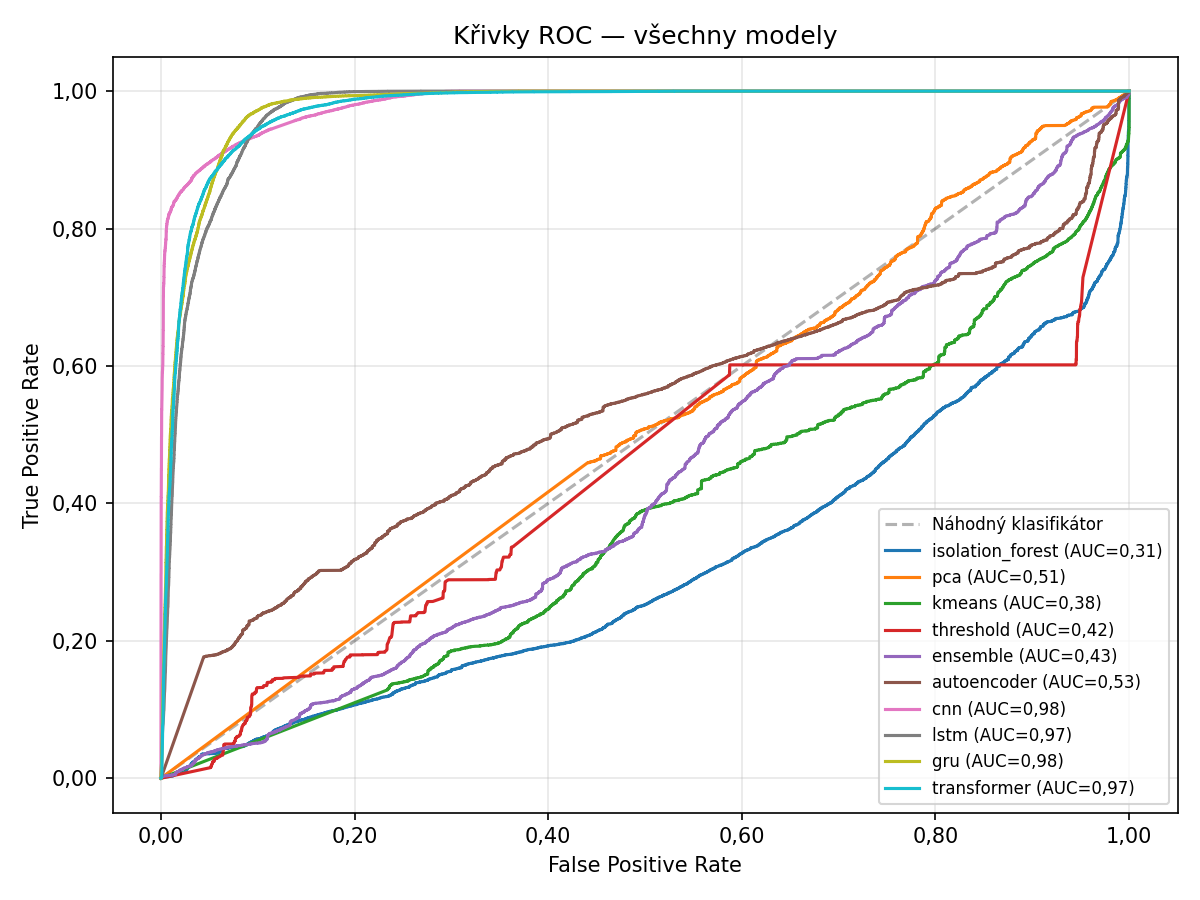
\includegraphics[width=0.85\textwidth]{roc_curves.png}
\caption{ROC křivky všech modelů na validačních datech}
\label{fig:roc-curves}
\end{figure}

Obrázek~\ref{fig:pr-curves} zobrazuje křivky závislosti přesnosti na úplnosti (precision--recall), které jsou v~kontextu nevyvážené datové sady informativnější než ROC, protože nezohledňují počet pravdivě negativních klasifikací \parencite{Ji2024}. CNN si udržuje přesnost nad 0{,}93 i~při úplnosti blížící se 0{,}95 (PR-AUC $= 0{,}99$). U~metod klasického strojového učení a~statistických přístupů přesnost klesá rychle s~rostoucí úplností; autoencoder a~PCA dosahují PR-AUC okolo~0{,}73, zatímco izolační les a~\texttt{ensemble} se pohybují pod~0{,}60. Křivky PR tak potvrzují, že rozdíl mezi modely hlubokého učení s~učitelem a~ostatními skupinami není artefaktem volby prahu, ale odráží skutečně odlišnou schopnost rozlišovat třídy.

\begin{figure}[htbp]
\centering
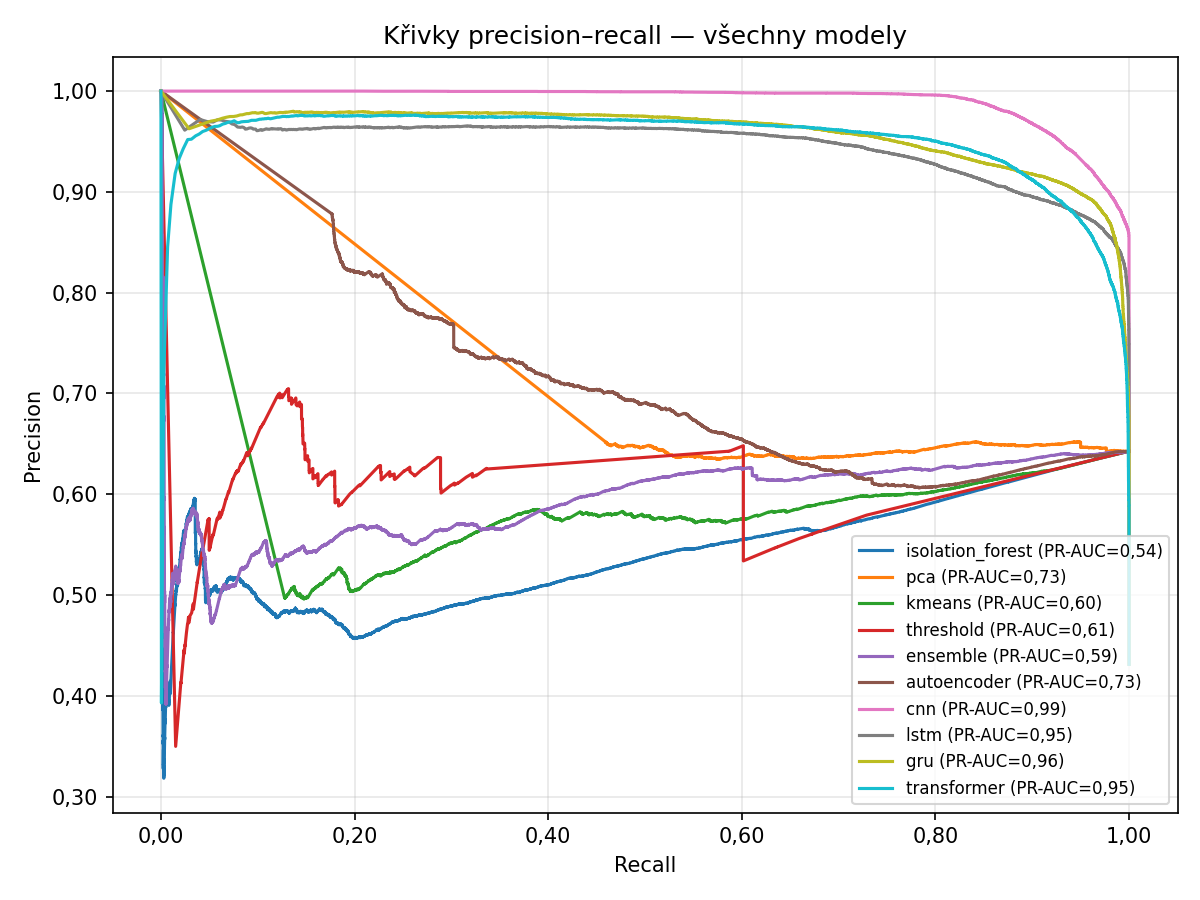
\includegraphics[width=0.85\textwidth]{pr_curves.png}
\caption{precision--recall křivky na validačních datech}
\label{fig:pr-curves}
\end{figure}

Obrázek~\ref{fig:metric-comparison} srovnává klíčové metriky (přesnost, úplnost, F1) formou skupinového sloupcového grafu pro deset detektorů; referenční model \texttt{baseline} je z~grafu vynechán, protože má nulovou přesnost, úplnost i~F1 a~nebyl by na měřítku 0--1 viditelný. Vizuálně je patrný skok v~F1 mezi klasickým strojovým učením a~statistickými metodami (nejvýše PCA s~0{,}61) a~modely hlubokého učení s~učitelem (CNN s~0{,}94). U~klasického strojového učení a~statistických metod je rovněž zřetelná disproporce mezi přesností a~úplností: prahování z-skóre dosahuje přesnosti~0{,}70, ale úplnosti pouhých~0{,}14, zatímco modely s~učitelem mají hodnoty obou metrik přibližně vyrovnané.

\begin{figure}[htbp]
\centering
% Pouze šířka řádku: kombinace width+height+keepaspectratio dříve vybírala menší měřítko a velikost se nezměnila.
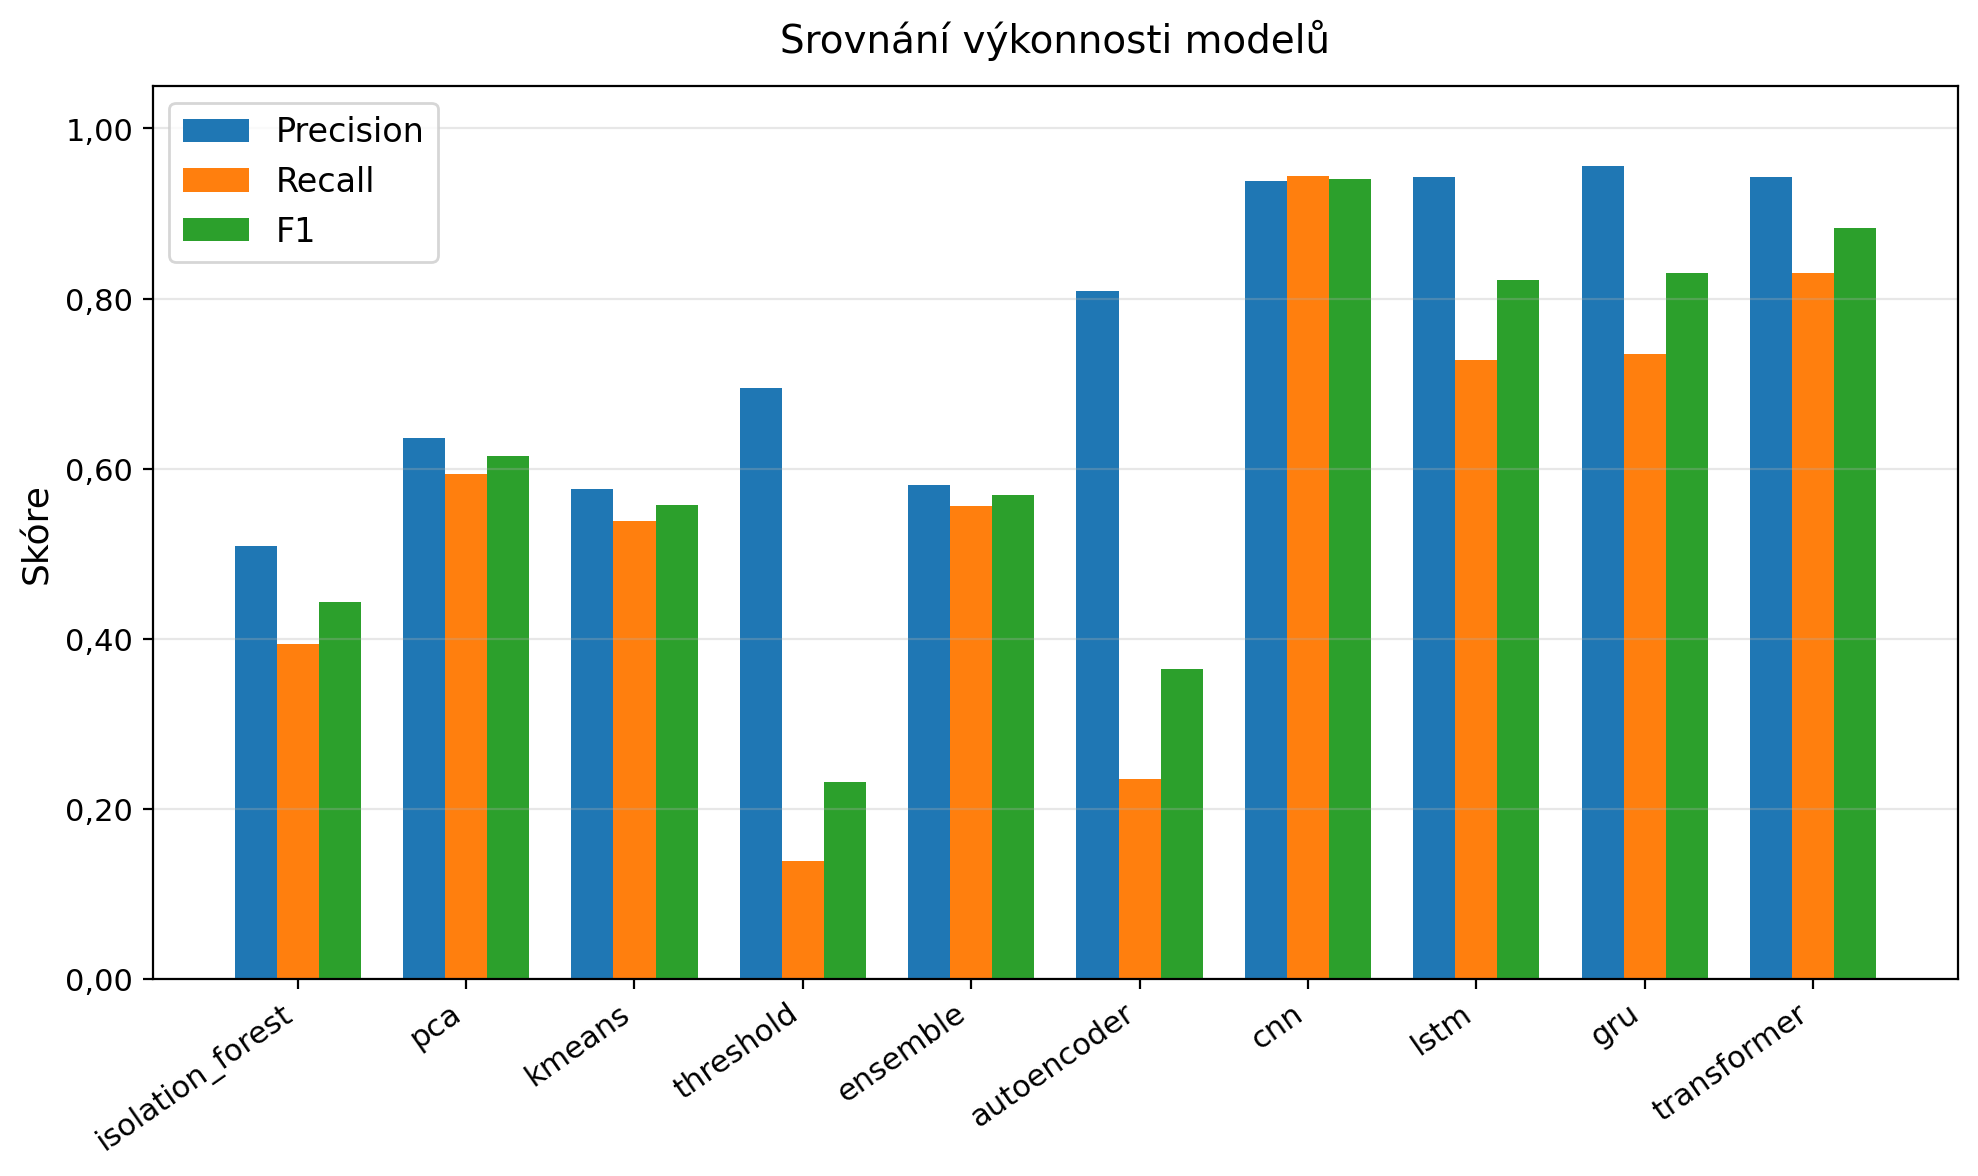
\includegraphics[width=\textwidth]{metric_comparison.png}
\caption[Srovnání precision, recall, F1 napříč modely]{Srovnání precision, recall a~F1 skóre napříč modely (bez referenčního baseline)}
\label{fig:metric-comparison}
\end{figure}

Obrázek~\ref{fig:confusion-matrices} představuje matice záměn jednotlivých modelů. U~CNN je patrná symetrie -- nízký počet jak falešně pozitivních, tak falešně negativních klasifikací. U~prahového modelu (\texttt{threshold}) naopak dominují falešně negativní chyby (28\,515 z~33\,121 anomálií), což potvrzuje omezenost jednorozměrného prahování na této datové sadě.

\begin{figure}[htbp]
\centering
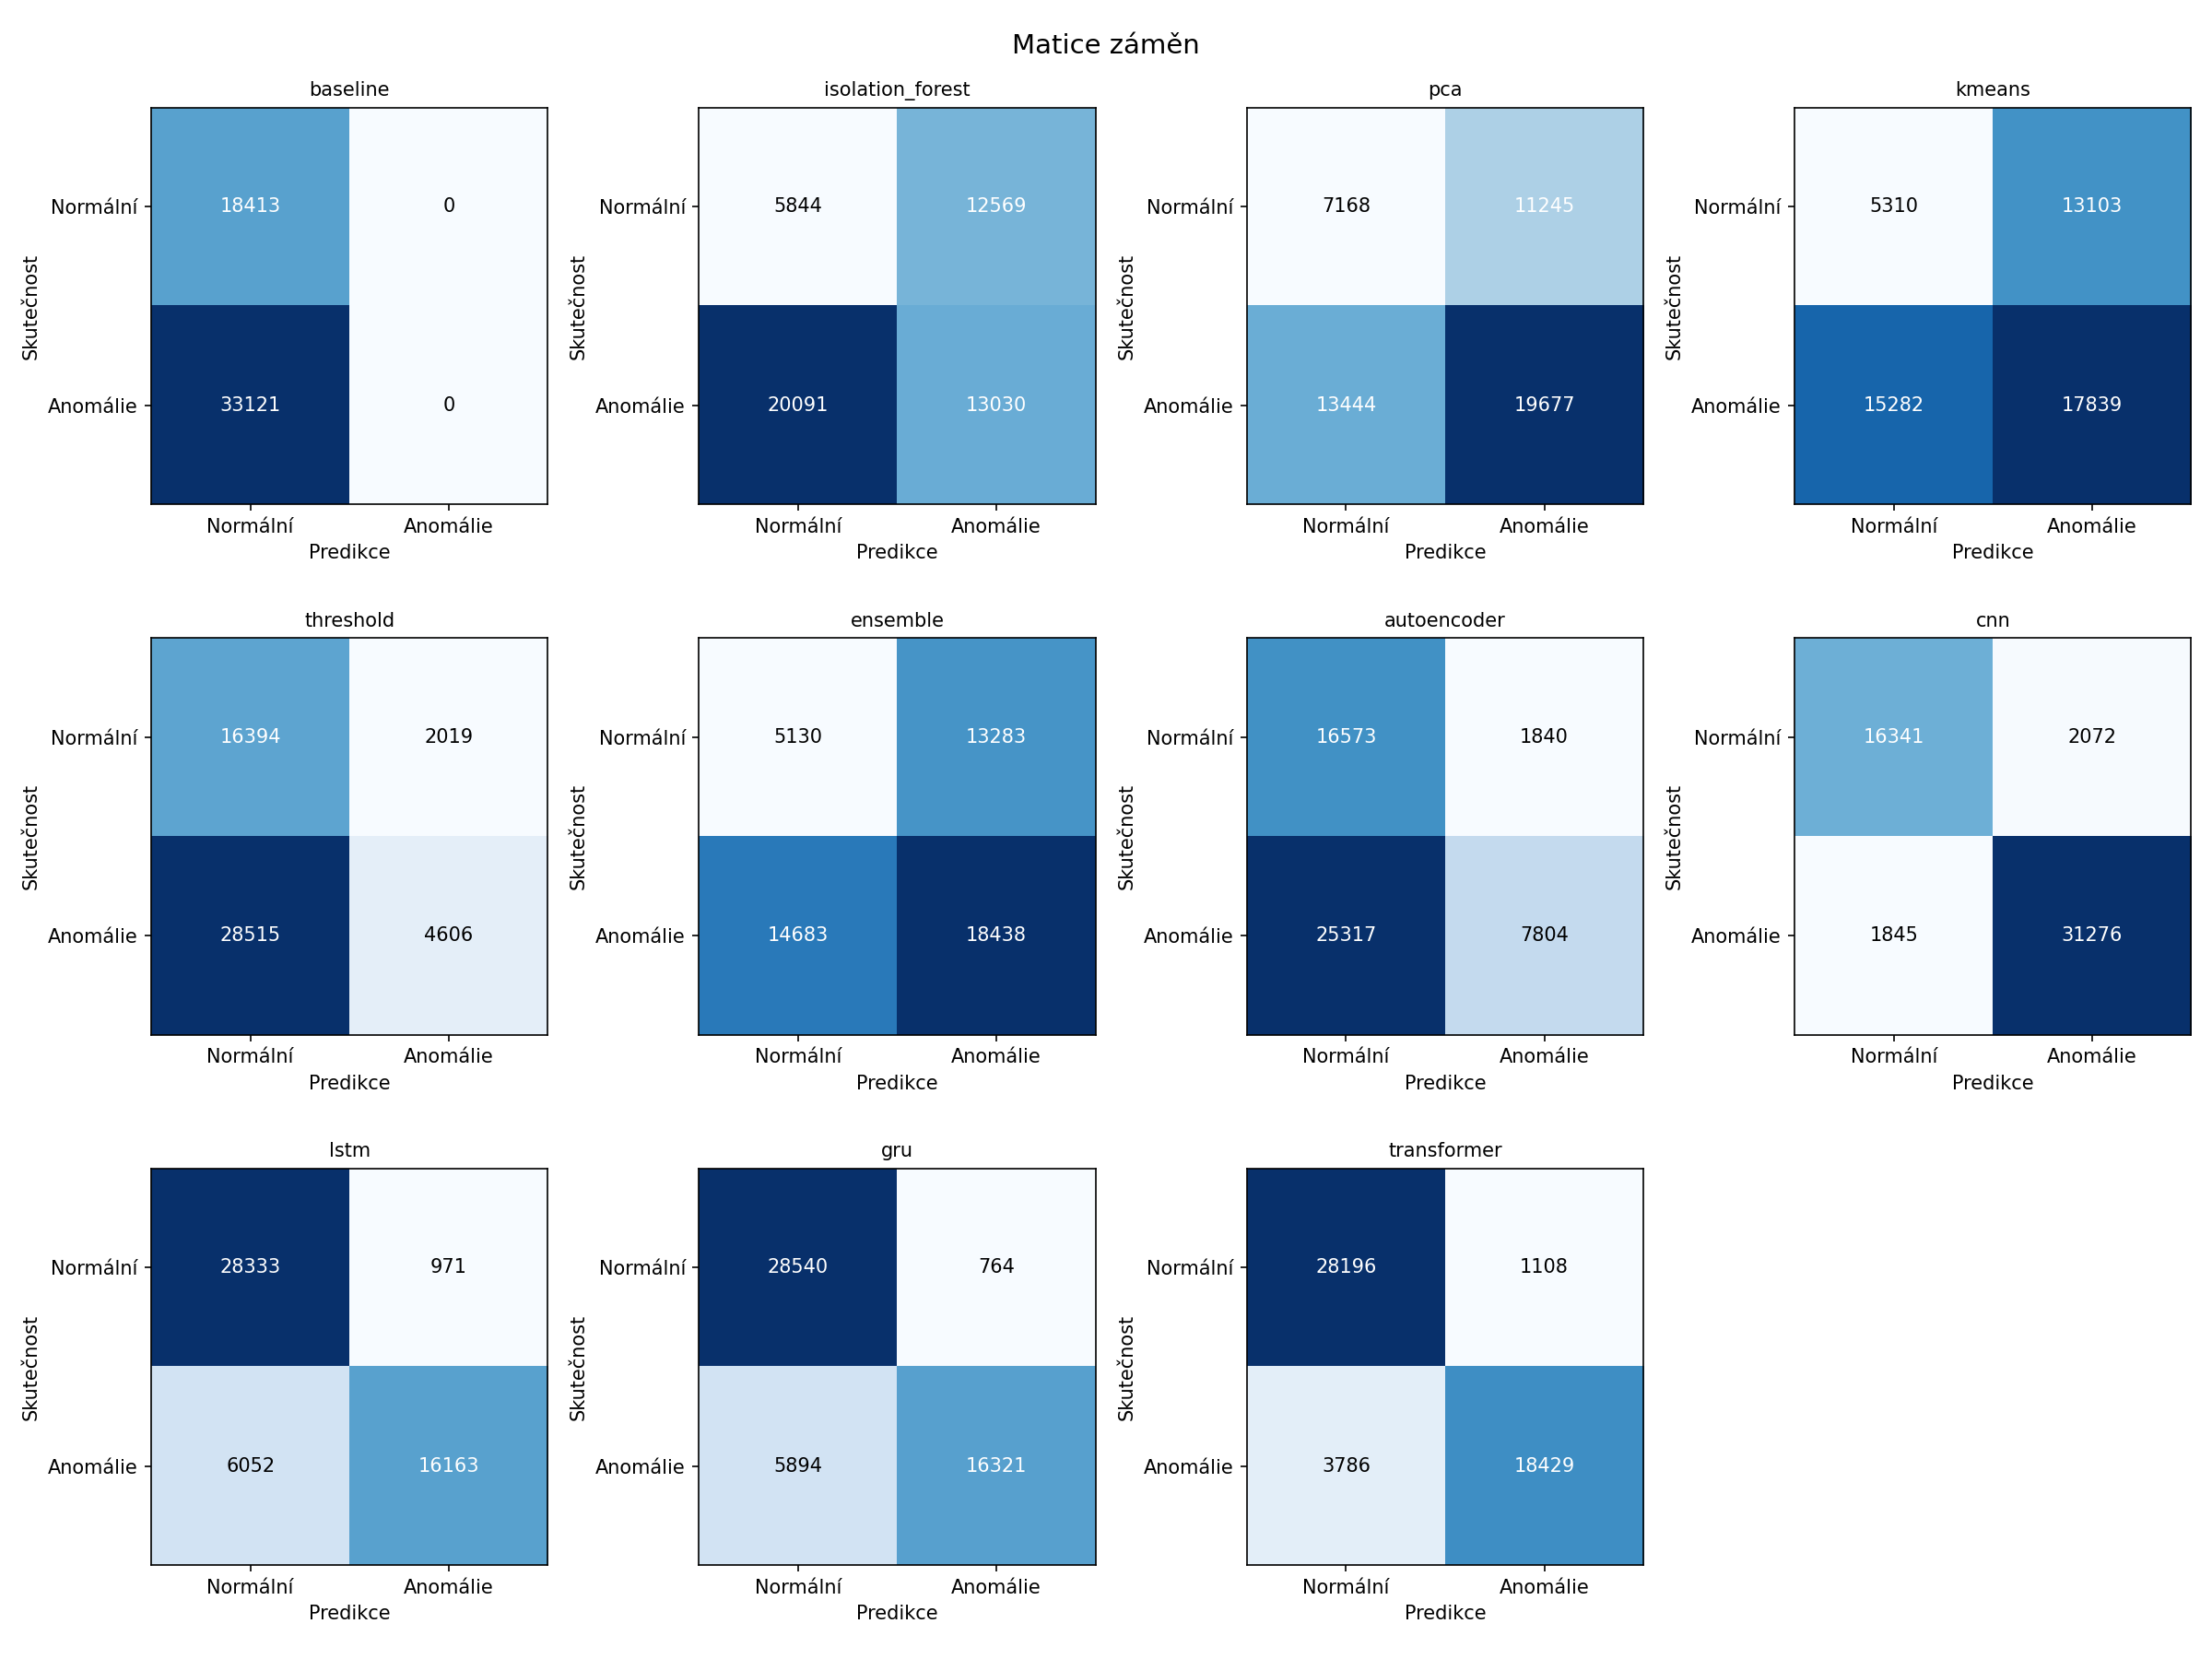
\includegraphics[width=0.95\textwidth]{confusion_matrices.png}
\caption{Matice záměn pro všechny vyhodnocené modely}
\label{fig:confusion-matrices}
\end{figure}

\section{Srovnání metod}
\label{sec:srovnani}

Tato sekce odpovídá na dílčí cíl~5 práce -- systematicky porovnat efektivitu tří skupin metod a~identifikovat situace, ve~kterých je použití hlubokého učení přínosné. Srovnání vychází z~metrik definovaných v~sekci~\ref{sec:metriky} a~z~kontrolovaného experimentu navrženého v~sekci~\ref{sec:design-experimentu}.

\subsection{Analýza skupinových metrik}
\label{sec:analyza-skupin}

Průměrné F1 v~jednotlivých skupinách na hlavním rozdělení dat činí: hluboké učení 0{,}768, klasické strojové učení 0{,}538 a~statistické/heuristické metody (bez baseline) 0{,}397. Rozdíly mezi skupinami jsou konzistentní: nejlepší model klasického strojového učení (PCA, F1 $= 0{,}61$) nedosahuje ani úrovně nejslabšího modelu hlubokého učení s~učitelem (LSTM, F1 $= 0{,}82$). Při vyřazení autoencoderu (model hlubokého učení bez učitele s~F1 $= 0{,}37$) průměr skupiny hlubokého učení vzroste na~0{,}869. Tyto výsledky jsou konzistentní s~literaturou \parencite{Barut2020}, kde modely hlubokého učení s~učitelem rovněž dominují na datových sadách s~příznaky na úrovni toku.

Z~hlediska úplnosti je situace analogická: průměrná úplnost modelů hlubokého učení s~učitelem je 0{,}809, klasického strojového učení 0{,}444 a~statistických metod 0{,}348 (obojí bez baseline). V~bezpečnostním kontextu je tento rozdíl kritický, protože nezachycená anomálie může mít závažnější důsledky než falešný poplach \parencite{OzkanOkay2021}.

Autoencoder představuje zajímavý hraniční případ: jako architektura hlubokého učení je řazen do příslušné skupiny, ale jeho režim učení bez učitele ho výkonnostně řadí blíže ke klasickému strojovému učení (F1 $= 0{,}37$ oproti PCA s~F1 $= 0{,}61$). To naznačuje, že přínos hlubokého učení plyne primárně z~trénování s~učitelem s~přímou optimalizací na klasifikační ztrátu, nikoli ze samotné neuronové architektury. Tento poznatek je konzistentní s~tématem T1 analýzy v~sekci~\ref{sec:tematicka-analyza}, kde míra supervize byla identifikována jako klíčový praktický diferenciátor metod.

Z~hlediska výpočetních nároků dosahuje CNN jako model bez časového kontextu nejvyššího skóre F1 ($0{,}94$), přičemž jeho klasifikační latence je nižší než u~sekvenčních modelů (viz sekce~\ref{sec:nn-dl}). To podporuje zjištění \textcite{Bakhshi2021}, že CNN je efektivní volbou v~situacích, kdy je rychlost klasifikace kritická. Sekvenční modely (Transformer, GRU, LSTM) dosahují nižšího F1 ($0{,}82$--$0{,}88$), protože přidaný časový kontext na této datové sadě nepřináší dostatečné zlepšení.

\subsection{Statistická významnost rozdílů mezi skupinami metod}
\label{sec:stat-vyznamnost}

Pro ověření hypotézy práce -- že metody hlubokého učení dosahují vyššího F1~skóre než metody klasického strojového učení i~statistické/heuristické metody -- byly použity testy popsané v~sekci~\ref{sec:stat-testovani}.

Globální test (Kruskal--Wallis). Pro každé z~$k=10$ opakování křížové validace byl spočten průměr F1 přes modely v~každé ze tří skupin. Kruskal--Wallisův test na takto získaných třiceti hodnotách (10 na skupinu) zamítl nulovou hypotézu shodných mediánů $H_0^{\mathrm{glob}}$: $H = 13{,}42$, $p = 0{,}0012$. Na hladině $\alpha = 0{,}05$ lze tedy konstatovat, že mezi třemi skupinami existuje statisticky významný rozdíl v~F1, a~je oprávněné přejít k~párovým testům ověřujícím směr.

Post-hoc jednostranné Wilcoxonovy testy s~Bonferroniho korekcí ($n = 3$ srovnání); první dvě srovnání přímo odpovídají hypotéze práce, třetí je doplňkové:
\begin{itemize}
\item Hluboké učení vs.~klasické strojové učení: $W = 52$, $p_{\mathrm{Bonf}} = 0{,}0146$ -- hluboké učení dosahuje vyššího F1 (průměrné fold-means: hluboké učení $= 0{,}737$, klasické strojové učení $= 0{,}491$).
\item Hluboké učení vs.~statistické: $W = 52$, $p_{\mathrm{Bonf}} = 0{,}0146$ -- hluboké učení dosahuje vyššího F1 (statistické: $0{,}361$).
\item Klasické strojové učení vs.~statistické (doplňkově): $W = 55$, $p_{\mathrm{Bonf}} = 0{,}0029$ -- klasické strojové učení dosahuje vyššího F1 než statistické metody.
\end{itemize}
Obě srovnání přímo ověřující hypotézu jsou na hladině $\alpha = 0{,}05$ statisticky významná i~po Bonferroniho korekci; hypotéza práce je tedy daty podpořena. Doplňkové srovnání klasického strojového učení se statistickými metodami navíc ukazuje, že ani tyto dvě skupiny nejsou mezi sebou zaměnitelné a existuje mezi nimi výkonnostní rozdíl.

Sekundární test bez autoencoderu -- při jeho vyloučení ze skupiny hlubokého učení (zbývají CNN, LSTM, GRU, Transformer) vzrůstá průměr fold-means na 0{,}799 a~statistická významnost se zvyšuje: hluboké učení s~učitelem vs.~klasické strojové učení $p_{\mathrm{Bonf}} = 0{,}0098$, hluboké učení s~učitelem vs.~statistické $p_{\mathrm{Bonf}} = 0{,}0098$.

Křížová validace pro statistické závěry byla provedena na náhodném podvzorku 8\,000 trénovacích toků (iniciální hodnota generátorů~42; u~časově seřazených dat zachován časový sled výběru), zatímco metriky v~tabulce~\ref{tab:metriky-vsechny} vycházejí z~trénování na úplné trénovací množině.

\section{Diskuse}
\label{sec:diskuse}

Předchozí sekce kvantifikovaly rozdíly mezi třemi skupinami metod na úrovni metrik a~statistických testů. Tato sekce interpretuje zjištění v~širším kontextu -- zasazuje výsledky do rámce existující literatury, analyzuje příčiny pozorovaných rozdílů a~diskutuje kvalitativní aspekty nasazení, které samotné F1~skóre nezachycuje.

\subsection{Interpretace výsledků v~kontextu literatury}
\label{sec:diskuse-literatura}

Dominance CNN (F1 $= 0{,}94$) mezi modely s~učitelem je konzistentní se závěry \textcite{Barut2020}, kteří na datových sadách s~příznaky na úrovni toku rovněž zaznamenali nejvyšší výkonnost u~modelů hlubokého učení s~učitelem. \textcite{Bakhshi2021} navíc potvrzují, že jednorozměrné konvoluční sítě kombinují vysokou klasifikační přesnost s~nízkou latencí, což je činí vhodnou volbou pro nasazení v~reálném čase. Výsledky experimentu toto pozorování replikují na nezávislé datové sadě s~odlišným příznakovým schématem.

Pozoruhodným zjištěním je, že sekvenční modely Transformer ($\text{F1} = 0{,}88$), GRU ($\text{F1} = 0{,}83$), LSTM ($\text{F1} = 0{,}82$) nedosahují výkonnosti CNN, přestože zachycují časové závislosti mezi toky. Tento výsledek pravděpodobně odráží specifika kanonického schématu: 17~příznaků agreguje statistiky na úrovni jednotlivých toků (průměrné velikosti paketů, mezipaketové intervaly, objemy), kde je většina rozlišující informací obsažena v~rámci jednoho toku. Časový kontext posuvného okna přináší jen malé zlepšení, které navíc nevykompenzuje ztrátu pozorování na okrajích sekvence a~odlišnou validační podmnožinu. Literatura tento jev explicitně nediskutuje, protože většina srovnávacích studií buď testuje pouze jeden typ architektury, nebo pracuje se surovými bajty místo agregovaných příznaků \parencite{Ji2024}.

Z~hlediska témat tematické analýzy (sekce~\ref{sec:tematicka-analyza}) výsledky experimentu potvrzují klíčový poznatek tématu T1 (míra supervize): režim učení je pro výkonnost detektoru rozhodující faktor, zatímco samotná architektura sítě má sekundární vliv. Tří-skupinové rozdělení metod navíc odhaluje, že metody klasického strojového učení (průměrné F1 $= 0{,}491$) se statisticky významně liší od statistických metod (F1 $= 0{,}361$), což by při dvouskupinovém dělení (hluboké učení vs.~ostatní) zůstalo skryté. Téma T3 (důkladnost validace) je naplněno provedením kontrolovaného experimentu na shodné datové sadě s~křížovou validací a~Kruskal--Wallisovým testem s~post-hoc korekcí, čímž se odstraňuje nestejnorodost podmínek, která ztěžuje porovnání výsledků v~rešeršovaných studiích.

\subsection{Vliv režimu učení na výkonnost}
\label{sec:diskuse-rezim-uceni}

Autoencoder jako model hlubokého učení bez učitele dosáhl F1 $= 0{,}37$, což je výrazně pod úrovní nejlepší metody klasického strojového učení -- PCA (F1 $= 0{,}61$). Tento výsledek zpochybňuje zjednodušenou představu, že neuronová architektura sama o~sobě zaručuje vyšší výkonnost. Příčina spočívá v~odlišnosti optimalizačních cílů: modely s~učitelem (CNN, LSTM, GRU, Transformer) optimalizují váženou binární křížovou entropii, která přímo penalizuje klasifikační chyby s~důrazem na úplnost; autoencoder naproti tomu minimalizuje rekonstrukční chybu (MSE), která je pouze nepřímým ukazatelem anomálie. PCA, ačkoli lineární, pracuje s~přímou rekonstrukční chybou ve vysvětlitelném podprostoru a~má vyšší nastavenou kontaminaci (0{,}5--0{,}6 oproti 0{,}1 u~autoencoderu), čímž zachytí větší podíl anomálních toků.

Citlivost na parametr kontaminace, identifikovaná v~sekci~\ref{sec:hrozby-validity} jako hrozba vnitřní validity, se v~experimentu projevila především u~metod bez učitele v~obou skupinách (hluboké i~klasické strojové učení). Hodnoty kontaminace 0{,}5--0{,}6 byly zvoleny na základě skutečného podílu anomálií v~UNSW-NB15; při výchozí hodnotě 0{,}1 by metody klasického strojového učení dosahovaly výrazně nižšího skóre~F1. Modely hlubokého učení s~učitelem jsou na tento parametr necitlivé, protože optimalizují klasifikační hranici přímo z~anotovaných dat. Tato asymetrie zvýhodňuje modely s~učitelem v~těch situacích, kdy skutečný podíl anomálií v~síťovém provozu není předem znám.

\subsection{Kvalitativní aspekty nasazení}
\label{sec:diskuse-kvalitativni}

F1~skóre a~ROC-AUC nezachycují několik aspektů, které jsou pro praktické nasazení detektorů podstatné. V~sekci~\ref{sec:hrozby-validity} bylo zmíněno, že tyto aspekty budou diskutovány kvalitativně; následující odstavce tuto diskusi poskytují.

Z~hlediska výpočetní náročnosti trvalo trénování všech jedenácti modelů přibližně 23{,}5~hodiny na pracovní stanici s~procesorem Intel Core i7 a~16~GB~RAM, přičemž většina času připadla na neuronové sítě. Metody klasického strojového učení a~statistické přístupy (izolační les, PCA, K-means, prahování, ensemble) se trénují řádově v~minutách, protože nevyžadují iterativní optimalizaci vah. Pro organizace s~omezenými výpočetními zdroji nebo potřebou častého přetrénování (například při adaptaci na nový provoz) představuje tento rozdíl praktické omezení nasazení metod hlubokého učení.

Latence při klasifikaci se liší v~závislosti na architektuře. CNN zpracovává jednotlivé toky nezávisle, takže klasifikace nového toku nevyžaduje čekání na akumulaci okna. Sekvenční modely (LSTM, GRU, Transformer) naproti tomu vyžadují posuvné okno 16~toků, což přidává zpoždění a~komplikuje nasazení v~prostředí s~požadavkem na klasifikaci v~reálném čase. Metody klasického strojového učení a~statistické přístupy mají zanedbatelnou klasifikační latenci.

Interpretovatelnost výstupů je další dimenzí, která ovlivňuje využitelnost detektoru v~bezpečnostních operacích. PCA umožňuje rozložit rekonstrukční chybu na příspěvky jednotlivých příznaků, čímž operátor získá informaci o~tom, které charakteristiky toku jsou neobvyklé. Izolační les identifikuje příznaky, na nichž byl anomální tok izolován. Neuronové sítě jsou v~tomto ohledu netransparentní -- bez dodatečných technik vysvětlitelné AI (XAI) nelze určit, proč model tok klasifikoval jako anomální. \textcite{Capuano2022} přitom upozorňují, že nasazení XAI v~bezpečnostním kontextu přináší riziko: transparentnost modelu může útočníkům poskytnout informace k~obcházení detekce. Téma T4 tematické analýzy (sekce~\ref{sec:ta-temata}) tyto provozní aspekty identifikovalo jako nedostatečně reflektované v~literatuře; prezentovaná diskuse tento deficit částečně zaplňuje na konkrétních experimentálních datech.

\subsection{Fenomén invertovaného ROC-AUC}
\label{sec:diskuse-roc}

Hodnoty ROC-AUC metod klasického strojového učení a~statistických přístupů pod~0{,}5 (izolační les 0{,}31; K-means 0{,}38; ensemble 0{,}43; prahování 0{,}42) byly popsány v~sekci~\ref{sec:graficke-vystupy}. Z~hlediska nasazení má tento jev praktický důsledek: spojitá skóre anomálie těchto modelů nelze přímo použít pro prioritizaci poplachů. Operátor SOC potřebuje nejen binární rozhodnutí (anomální / normální), ale i~řazení podezřelých toků podle míry podezřelosti, aby mohl efektivně alokovat čas na analýzu nejvážnějších incidentů.

Modely s~učitelem tento problém nemají -- sigmoidální výstup neuronových sítí přímo reprezentuje pravděpodobnost anomálie a~ROC-AUC přesahuje 0{,}97 u~všech čtyř modelů. CNN s~ROC-AUC $= 0{,}98$ a~PR-AUC $= 0{,}99$ poskytuje spojité skóre s~korektní orientací a~vysokou rozlišovací schopností v~celém rozsahu prahů. Pro organizace, které potřebují prioritizovanou frontu poplachů (nikoli pouze binární klasifikaci), představují modely s~učitelem jedinou spolehlivou volbu z~testovaných metod.

Invertované ROC-AUC metod klasického strojového učení a~statistických přístupů pravděpodobně souvisí s~konvencí vnitřních skóre (izolační les například přiřazuje anomáliím kratší průměrnou cestu ke~kořeni stromu, tj.~nižší číselné skóre) a~s~interakcí mezi vysokou prevalencí anomálií v~datové sadě a~transformací skóre na~pravděpodobnostní škálu. Při nižší prevalenci anomálií by se orientace skóre mohla změnit, což podtrhuje závislost výsledků na charakteristikách datové sady diskutovanou v~sekci~\ref{sec:omezeni-vysledku}.

\section{Typové situace pro volbu detekční metody}
\label{sec:identifikace-situaci}

Tato sekce přímo naplňuje druhou část dílčího cíle~5 -- identifikovat situace, ve~kterých je použití hlubokého učení přínosné. Na základě výsledků v~tabulce~\ref{tab:metriky-vsechny}, grafických výstupů a~statistických testů v~předchozí sekci lze identifikovat tři typové situace:

\begin{enumerate}
\item Dostupná anotovaná data a~požadavek na vysokou úplnost i~přesnost:

V~tomto případě je nasazení modelů hlubokého učení s~učitelem (CNN, Transformer) jednoznačně přínosné. CNN dosáhl F1 $= 0{,}94$ oproti nejlepšímu modelu klasického strojového učení (PCA, F1 $= 0{,}61$) -- absolutní rozdíl 33~procentních bodů. Pro bezpečnostní operace, kde je kritická úplnost, představuje nárůst z~$\text{R} = 0{,}59$ (PCA) na $\text{R} = 0{,}94$ (CNN) zachycení dalších přibližně 11\,600 anomálních toků z~33\,121.

\item Omezené výpočetní zdroje nebo požadavek na interpretovatelnost:

PCA a~ensemble zůstávají relevantní jako interpretovatelné alternativy. PCA model je transparentní (rekonstrukční chyba ve vysvětlitelném podprostoru), vyžaduje minimální výpočetní zdroje a~dosahuje nejlepšího F1 mezi metodami klasického strojového učení. V~prostředích bez GPU nebo tam, kde je nutné zdůvodnit každý poplach operátorovi, může PCA představovat přijatelný kompromis. Statistické metody (prahování) jsou naopak vhodné pouze jako první filtrační vrstva díky extrémně nízké úplnosti.

\item Absence anotovaných dat (režim bez učitele):

V~tomto scénáři jsou metody hlubokého a~klasického strojového učení výkonnostně srovnatelné: autoencoder ($\text{F1} = 0{,}37$) vs.\ PCA ($\text{F1} = 0{,}61$). PCA paradoxně překonává autoencoder, pravděpodobně proto, že lineární rekonstrukce lépe odráží strukturu kanonických příznaků než nelineární transformace autoencoderu s~nízkou kontaminací. Při učení bez učitele tedy nasazení metody hlubokého učení nepřináší přidanou hodnotu, metoda klasického strojového učení je preferovaná.
\end{enumerate}

\section{Omezení interpretace výsledků}
\label{sec:omezeni-vysledku}

Tato sekce navazuje na hrozby validity identifikované v~sekci~\ref{sec:hrozby-validity} a~konkretizuje jejich dopad na získané výsledky. Podstatná je zde hrozba externí validity~-- experiment byl proveden na jedné datové sadě.

Mapování UNSW-NB15 do kanonického schématu je přibližné (viz tabulka~\ref{tab:feature-mapping} v~sekci~\ref{sec:kanonicke-schema}); absolutní hodnoty metrik proto nelze bez dalšího zpracování vztahovat na čistě HTTPS metadata v~produkční síti. Výsledky slouží primárně k~relativnímu srovnání implementovaných detektorů v~rámci stejného postupu zpracování.

Vysoký podíl anomálií (64\,\%) v~datové sadě neodpovídá typickému produkčnímu provozu, kde anomálie tvoří řádově promile toků. Při nasazení na data s~nižší prevalencí by se zvýšil podíl falešných pozitiv a~snížila pozitivní prediktivní hodnota (PPV), zejména u~metod bez učitele. Modely s~učitelem by v~takovém případě potřebovaly přetrénování na reprezentativních datech. Vysoká prevalence anomálií rovněž ovlivňuje nastavení parametru kontaminace u~metod bez učitele (viz sekce~\ref{sec:predzpracovani} a~\ref{sec:tradicni-algoritmy}), která byla v~tomto experimentu záměrně nastavena na~0{,}5--0{,}6; při nižší prevalenci by výchozí hodnoty kontaminace (typicky~0{,}1) mohly být přiměřenější.

Rozsah pokrytých scénářů je omezen na kategorie útoků obsažené v~UNSW-NB15 (devět typů), které nelze považovat za vyčerpávající reprezentaci současných kybernetických hrozeb. Datová sada neobsahuje například moderní varianty ransomwaru komunikujícího přes TLS ani útoky typu domain fronting (viz taxonomie v~sekci~\ref{sec:taxonomie-utoku}), jejichž detekce na úrovni toků je otevřeným problémem \parencite{Ferdous2023}.

Hodnoty ROC-AUC metod klasického strojového učení pod~0{,}5 (viz sekce~\ref{sec:graficke-vystupy}) naznačují, že spojitá skóre anomálií těchto modelů nemají na dané datové sadě korektní orientaci. Tento jev omezuje možnost použít metody klasického strojového učení bez učitele pro prahově nezávislé hodnocení rizika, přestože jejich binární klasifikační výkon (po nastavení prahu kontaminací) je přijatelný.

Výkonnost všech modelů závisí na kvalitě a~reprezentativnosti trénovacích dat. V~reálném prostředí se statistické vlastnosti provozu mění v~čase (concept drift, viz sekce~\ref{sec:rezimy-uceni}), což může vést k~postupné degradaci přesnosti modelů trénovaných na statické datové sadě \parencite{Qing2025}. Experiment v~této práci tento jev nezachycuje, protože trénovací i~validační data pocházejí ze stejného sběru; ověření robustnosti vůči posunu distribucí by vyžadovalo časovou řadu měření nebo simulaci driftu. Syntetické prostředí popsané v~sekci~\ref{sec:exp-prostredi} by v~budoucnu mohlo sloužit jako základ pro generování provozu s~postupně se měnícími charakteristikami, pokud bude rozšířeno o~generátor s~realistickými paketovými statistikami (viz sekce~\ref{sec:omezeni-synteticke}).

% \include{kap04}
% \include{...}
% \include{...}
\chapter*{Závěr}
\addcontentsline{toc}{chapter}{Závěr}

\section*{Shrnutí práce}
\addcontentsline{toc}{section}{Shrnutí práce}

Diplomová práce se zabývala detekcí anomálií v~šifrované síťové komunikaci a~systematickým srovnáním tří skupin detekčních metod: hlubokého učení, klasického strojového učení a~statistických/heuristických přístupů. V~rešeršní části (kapitola~\ref{chap:reserse}) bylo analyzováno 18~zdrojů pokrývajících šifrovací protokoly, taxonomii útoků, metody hlubokého učení, klasického strojového učení a~statistické detektory; tematická analýza podle \textcite{Braun2006} identifikovala čtyři průřezová témata, která strukturovala navazující návrh experimentu. V~metodické části (kapitola~\ref{chap:metodika}) bylo v~rámci strategie Design Science Research \parencite{Peffers2007} navrženo dvouúrovňové experimentální prostředí -- syntetický integrační režim pro ověření řetězce zpracování a~reprodukovatelný režim přehrávání srovnávacích dat -- a~implementován prototyp detekčního systému se společným rozhraním pro jedenáct modelů ze tří skupin. Kontrolovaný experiment na datové sadě UNSW-NB15 (kapitola~\ref{chap:vysledky}) prokázal statisticky významný rozdíl ve výkonnosti všech tří skupin a~umožnil identifikovat situace, ve~kterých je nasazení výpočetně náročnějšího hlubokého učení přínosné.

\section*{Shrnutí výstupů vzhledem k cílům práce}
\addcontentsline{toc}{section}{Shrnutí výstupů vzhledem k cílům práce}

Hlavním cílem práce bylo navrhnout a implementovat systém pro detekci anomálií
v šifrované síťové komunikaci s využitím metod umělé inteligence a systematicky porovnat tři
skupiny detekčních metod v experimentálním prostředí. Naplnění hlavního cíle je podloženo splněním pěti dílčích cílů:

\begin{itemize}
\item Identifikovat a~analyzovat aktuální metody hlubokého učení, klasického strojového učení a~statistické metody vhodné pro detekci anomálií v~šifrovaném provozu na základě rešerše literatury:

Rešerše v~kapitole~\ref{chap:reserse} pokrývá metody hlubokého učení (CNN, LSTM, GRU, Transformer, autoencoder), klasického strojového učení (izolační les, PCA, K-means) i~statistické přístupy (prahování, pravidlové metody) včetně teoretického srovnání. Tematická analýza propojila poznatky z~literatury s~návrhem experimentu.

\item Navrhnout experimentální prostředí umožňující sběr, generování a~validaci dat síťových toků pro testování detekčních metod:

V~sekci~\ref{sec:exp-prostredi} je popsáno dvouúrovňové prostředí: syntetický integrační režim pro ověření řetězce zpracování a~režim přehrávání srovnávacích dat. Původní záměr generovat realistický útočný provoz se ukázal jako rozsáhlý výzkumný problém přesahující rámec práce (viz sekce~\ref{sec:omezeni-synteticke}); místo toho byl implementován reprodukovatelný řetězec zpracování nad veřejnou datovou sadou UNSW-NB15. Tento přechod je obhajitelný, protože srovnání detektorů na shodném příznakovém prostoru zůstává platné a~integrační prostředí je ponecháno jako základ pro budoucí rozšíření.

\item Implementovat prototyp detekčního systému využívajícího vybrané algoritmy ze všech tří skupin metod:

Balíček \texttt{detection-mechanisms} implementuje jedenáct detektorů se společným rozhraním (\texttt{fit}, \texttt{predict}, \texttt{predict\_scores}), registr modelů a~příkazovou utilitu se třemi režimy provozu (sekce~\ref{sec:implementace}). Architektura umožňuje snadné přidávání nových modelů.

\item Vyhodnotit účinnost implementovaných přístupů na připravených datech pomocí standardních metrik: přesnost, úplnost, F1~skóre a~ROC křivka:

Všech jedenáct modelů bylo vyhodnoceno na validační množině s~metrikami přesnost, úplnost, F1, celková přesnost klasifikace, ROC-AUC a~PR-AUC (tabulka~\ref{tab:metriky-vsechny}). Doplňkově byly vygenerovány křivky ROC, PR a~matice záměn.

\item Systematicky porovnat efektivitu tří skupin metod a~identifikovat situace, ve~kterých je použití hlubokého učení přínosné:

Sekce~\ref{sec:srovnani} systematicky porovnává tři skupiny na úrovni skupinových průměrů i~statistických testů; sekce~\ref{sec:identifikace-situaci} identifikuje tři typové situace lišící se dostupností anotovaných dat a~požadavky na interpretovatelnost.
\end{itemize}

\section*{Ověření hypotézy}
\addcontentsline{toc}{section}{Ověření hypotézy}

Hypotéza práce zněla: metody hlubokého učení dosahují vyššího F1~skóre při detekci anomálií v~šifrovaném provozu než metody klasického strojového učení i~statistické/heuristické metody. Ověření proběhlo dvoustupňově na deseti opakováních křížové validace (viz sekce~\ref{sec:stat-testovani}). Globální Kruskal--Wallisův test zamítl nulovou hypotézu shodných mediánů F1 ($H = 13{,}42$, $p = 0{,}0012$) na hladině významnosti $\alpha = 0{,}05$. Jednostranné post-hoc Wilcoxonovy testy s~Bonferroniho korekcí potvrdily samotnou hypotézu práce: hluboké učení dosáhlo vyššího F1 než klasické strojové učení ($p_{\mathrm{Bonf}} = 0{,}0146$) i~než statistické/heuristické metody ($p_{\mathrm{Bonf}} = 0{,}0146$). Průměrné F1 hlubokého učení činilo 0{,}737, klasického strojového učení 0{,}491 a~statistických metod 0{,}361; při vyřazení autoencoderu průměr hlubokého učení s~učitelem vzrostl na 0{,}799. Hypotéza byla tedy na zvolené datové sadě UNSW-NB15 podpořena daty, přičemž zobecnění na jiné datové sady a~síťová prostředí vyžaduje další validaci (viz sekce~\ref{sec:omezeni-vysledku}).

\section*{Přínosy práce}
\addcontentsline{toc}{section}{Přínosy práce}

Práce přináší konkrétní výstupy využitelné jak pro navazující výzkum, tak pro praxi bezpečnostních týmů organizací:

\begin{itemize}
\item Systematická analýza a~srovnání metod:

Rešerše 18~zdrojů s~tematickou analýzou poskytuje ucelený přehled metod hlubokého učení, klasického strojového učení a~statistických přístupů pro detekci anomálií v~šifrovaném provozu a~jejich vhodnosti pro analýzu bez narušení soukromí uživatelů.

\item Reprodukovatelné experimentální prostředí:

Dvouúrovňové prostředí (syntetický integrační režim a~režim přehrávání srovnávacích dat) s~kanonickým schématem 17~příznaků umožňuje reprodukovatelné testování detekčních metod na datech síťových toků a~může sloužit jako základ pro další výzkum.

\item Funkční prototyp detekčního systému:

Balíček \texttt{detection-mechanisms} se společným rozhraním pro jedenáct modelů demonstruje modulární architekturu, která umožňuje snadné přidávání nových detektorů a~po úpravách může být integrována do bezpečnostních nástrojů typu IDS/IPS.

\item Kvantifikované srovnání s~identifikací rozhodovacích situací:

Kontrolovaný experiment na UNSW-NB15 prokázal statisticky významný rozdíl mezi všemi třemi skupinami metod (Kruskal--Wallisův test, $p = 0{,}0012$; post-hoc párové Wilcoxonovy testy potvrdily rozdíly mezi každou dvojicí) a~identifikoval tři typové situace (sekce~\ref{sec:identifikace-situaci}), v~nichž se doporučení pro volbu metody liší podle dostupnosti anotovaných dat a~požadavků na interpretovatelnost.

\item Praktická doporučení pro bezpečnostní týmy:

Výsledky poskytují provozovatelům podnikových sítí a~SOC týmům podklady pro volbu detekčních technologií: v~režimu s~učitelem dosáhl CNN model F1\,=\,0{,}94, zatímco v~režimu bez učitele metody klasického strojového učení (izolační les, PCA) dosahují srovnatelné výkonnosti s~hlubokým učením při nižší výpočetní náročnosti.
\end{itemize}

\section*{Omezení a doporučení}
\addcontentsline{toc}{section}{Omezení a doporučení}

Hlavní omezení experimentu jsou podrobně diskutována v~sekcích~\ref{sec:diskuse} a~\ref{sec:omezeni-vysledku}. Zde jsou shrnuta z~nich ta nejpodstatnější:

\begin{itemize}
\item Jedna datová sada: experiment byl veden výhradně na UNSW-NB15 s~jednou pevnou iniciální hodnotou generátorů. Zobecnění výsledků na jiné datové sady a~síťová prostředí vyžaduje křížovou validaci.

\item Aproximativní mapování příznaků: kanonické schéma 17~příznaků vzniklo aproximativním mapováním z~UNSW-NB15, která neobsahuje čistě HTTPS provoz. Přímá přenositelnost na moderní TLS~1.3 toky je tím omezena.

\item Nevyvážené zastoupení tříd: podíl anomálií v~experimentální sadě (64\,\%) neodpovídá typickému produkčnímu provozu, kde je podíl anomálií výrazně nižší. Absolutní hodnoty metrik je proto třeba interpretovat s~ohledem na laboratorní charakter experimentu.

\item Neotestovaný concept drift: vliv postupné změny statistických vlastností provozu nebyl experimentálně ověřen; modely byly trénovány a~testovány na statickém snímku dat.

\item Integrační prostředí bez realistických útoků: implementace simulátoru útoků v~syntetickém integračním režimu se nepodařila realizovat v~plném rozsahu (viz sekce~\ref{sec:omezeni-synteticke}), čímž nebylo dosaženo end-to-end validace v~plně kontrolovaném prostředí.
\end{itemize}

Relativní srovnání detektorů na shodném vstupu nicméně zůstává platné a~výsledky představují spolehlivý základ pro navazující výzkum.

\section*{Možnosti dalšího výzkumu}
\addcontentsline{toc}{section}{Možnosti dalšího výzkumu}

Navazující výzkum se může ubírat několika směry:

\begin{itemize}
\item Křížová validace na dalších datových sadách, především CICIDS2017, pro kterou je normalizační skript v~repozitáři připraven, avšak nižší pokrytí kanonického schématu (59\,\%) vyžaduje úpravu příznakového prostoru.

\item Rozšíření syntetického prostředí o~generátor provozu na úrovni paketů s~realistickými statistikami velikostí a~mezipaketových intervalů, čímž by se umožnilo trénování a~validace v~podmínkách bližších produkčnímu nasazení.

\item Testování odolnosti modelů vůči změnám v distribuci dat (concept drift) na časových řadách nebo pomocí uměle vyvolaného driftu – důležité pro ověření použitelnosti v~reálném prostředí, kde se vlastnosti sítě průběžně mění.

\item Zkoumání kombinací detektorů zahrnujících modely hlubokého učení s~metodami klasického strojového učení a~statistickými přístupy, které by mohly nabídnout vyšší robustnost při zachování interpretovatelnosti.

\item Ověření prototypu v~reálném síťovém provozu s~měřením latence a~výpočetní náročnosti, což by doplnilo laboratorní výsledky o~praktickou perspektivu nasaditelnosti.
\end{itemize}

Výsledky práce potvrzují, že metody hlubokého učení přinášejí v~režimu učení s~učitelem měřitelný přínos pro detekci anomálií v~šifrované komunikaci, avšak jejich nasazení není univerzálně výhodnější než metody klasického strojového učení a~statistické přístupy. Volba detekční metody by měla vycházet z~dostupnosti anotovaných dat, požadavků na interpretovatelnost a~výpočetních zdrojů konkrétního prostředí -- tři typové situace identifikované v~sekci~\ref{sec:identifikace-situaci} poskytují k~tomuto rozhodnutí strukturovaný podklad.


\include{literatura}

\part*{Přílohy}
\appendix
\chapter{Dokumentace využití nástrojů AI}
\label{app:ai-usage}

V~souladu s~prohlášením k~využití AI jsou v~této příloze dokumentovány konkrétní způsoby, rozsah a~části práce, ve~kterých byly nástroje umělé inteligence použity.

\section*{Zlepšení gramatiky a jazykového stylu}

\begin{description}
\item[Nástroj:] Cursor \parencite{Cursor2026} s~jazykovým modelem Claude 4.6 Opus \parencite{Anthropic2025}
\item[Části práce:] Celý text diplomové práce (úvod, kapitoly~\ref{chap:reserse}--\ref{chap:vysledky}, závěr)
\item[Rozsah:] Stylistické korekce dílčích vět a~odstavců -- oprava gramatických chyb, hledání správných překladů odborných termínů do češtiny, úprava interpunkce a~formulací pro akademický styl. Nejednalo se o~přepisování celých pasáží; nástroj byl použit jako pokročilá kontrola pravopisu a~stylu.
\item[Vlastní přínos:] Veškerý odborný obsah, struktura argumentace, volba a~kritické zhodnocení citovaných zdrojů a~závěry jsou vlastním dílem. Výsledné znění každého odstavce bylo zkontrolováno a~v~případě potřeby upraveno.
\end{description}

\section*{Shrnutí literatury}

\begin{description}
\item[Nástroj:] Perplexity \parencite{Perplexity2026} s~jazykovým modelem Claude 4.6 Sonnet \parencite{Anthropic2025}
\item[Části práce:] Rešerše (kapitola~\ref{chap:reserse})
\item[Rozsah:] Stručná sumarizace obsahu nalezených zdrojů jako podklad pro vlastní zpracování. Vyhledávání zdrojů bylo provedeno samostatně v~databázích IEEE Xplore, SpringerLink, ACM Digital Library a~Google Scholar; nástroj AI byl využit pouze ke shrnutí obsahu již identifikovaných publikací.
\item[Vlastní přínos:] Vyhledání a~výběr konečné sady zdrojů, jejich kritické zhodnocení, provedení tematické analýzy podle \textcite{Braun2006}, syntéza závěrů a~propojení poznatků s~návrhem experimentu byly provedeny samostatně. Všechny citace byly ověřeny vůči původním publikacím.
\end{description}

\section*{Generování části zdrojových kódů}

\begin{description}
\item[Nástroj:] Cursor \parencite{Cursor2026} s~jazykovým modelem Claude 4.6 Opus \parencite{Anthropic2025}
\item[Části práce:] Zdrojový kód detekčního systému a~experimentálního prostředí
\item[Rozsah:] Generování pomocných skriptů, testů, vizualizací a~pipeline pro sestavení balíčku. Nástroj byl využit k~urychlení implementace dílčích komponent; výsledný kód byl vždy zkontrolován a~upraven.
\item[Vlastní přínos:] Celková architektura systému (společné rozhraní detektorů, registr modelů, kanonické schéma příznaků), volba algoritmů a~jejich hyperparametrů, návrh experimentálního protokolu včetně volby metrik a~statistických testů, rozhodnutí o~přechodu ze syntetického prostředí na srovnávací data, interpretace výsledků a~formulace závěrů jsou vlastním dílem. Konkrétně: definice společného návrh kanonického schématu 17~příznaků pro normalizaci datových sad, design dvouúrovňového experimentálního prostředí, konfigurace křížové validace a~volba Wilcoxonova testu pro párové srovnání. Veškerý vygenerovaný kód byl zkontrolován, testován a~v~řadě případů přepracován.
\end{description}

\chapter{Obsah přiloženého repozitáře}
\label{app:repository}

Zdrojové kódy, konfigurační soubory, experimentální skripty a~výsledky experimentu jsou součástí přiloženého repozitáře. Struktura repozitáře je popsána v~tabulce~\ref{tab:struktura-repozitare} v~kapitole~\ref{chap:metodika}; zde je uveden přehled hlavních komponent a~způsob reprodukce experimentu.

\section*{Hlavní komponenty}

\begin{description}
\item[\texttt{detection-mechanisms/}] Hlavní Python balíček obsahující implementaci všech jedenácti detektorů ze tří skupin (hluboké učení, klasické strojové učení, statistické), evaluační metriky, statistické testy a~vizualizace.
\item[\texttt{testing-environment/}] Kontejnerové testovací prostředí -- generátor syntetického provozu, přijímač a~agregátor toků, přehrávač srovnávacích dat.
\item[\texttt{experiments/}] Řízení experimentálního běhu (\texttt{run\_experiment.py}), výstupní metriky a~grafy v~\texttt{results/}.
\item[\texttt{tex/}] Zdrojové texty diplomové práce v~\LaTeX{u}.
\item[\texttt{Makefile}] Automatizace úloh \texttt{make} příkazy \texttt{install-all}, \texttt{prepare-data}, \texttt{evaluate-all}.
\end{description}

\section*{Reprodukce experimentu}

\begin{enumerate}
\item \texttt{make install-all} -- instalace závislostí.
\item \texttt{make prepare-data} -- stažení a~normalizace UNSW-NB15.
\item \texttt{make evaluate-all} -- spuštění experimentu pro všech 11~modelů včetně křížové validace.
\end{enumerate}

Iniciální hodnoty generátorů jsou fixovány na~42; výsledky jsou reprodukovatelné na shodné konfiguraci (Python~3.10, Linux).

\section*{Veřejné úložiště}

Zdrojové kódy, \LaTeX{} text práce i~experimentální data jsou veřejně dostupné na:
\begin{center}
\url{https://github.com/dashwoood/diploma}
\end{center}

% \include{...}
% \include{...}

\end{document}
